\documentclass[12pt,a4paper]{report}
\usepackage[T1]{fontenc}

\usepackage{amsmath,amssymb,amsfonts} 
\usepackage{booktabs}           
\usepackage{geometry}           
\usepackage{xcolor}             
\usepackage{hyperref}
\usepackage{seqsplit}           
\usepackage{setspace}           
\usepackage{graphicx}           
\graphicspath{{../latex_assets/}{latex_assets/}{./latex_assets/}{../}{./}}
\usepackage{array}
\usepackage{longtable}              
\usepackage{caption}            
\usepackage{subcaption}         
\usepackage{listings}           
\usepackage{enumitem}           
\usepackage{fancyhdr}           
\usepackage{cite}               
\usepackage{bm}                 
\usepackage{indentfirst}        
\usepackage{algorithm}          
\usepackage{algpseudocode}      
\usepackage{amsthm}             
\newtheorem{proposition}{Proposition}
\newtheorem{remark}{Remark}
\usepackage{adjustbox}
\usepackage{silence}
\WarningsOff[caption]
\WarningFilter{hyperref}{Token not allowed in a PDF string}
\WarningFilter{hyperref}{Difference (2) between bookmark levels}
\WarningFilter{latex}{`h' float specifier changed to `ht'}
\WarningFilter{latex}{Float too large for page}
\PassOptionsToPackage{hyperfootnotes=false}{hyperref}
\newcommand{\missingfigure}[1]{%
    \fbox{\parbox[c][4cm][c]{0.9\linewidth}{\centering
    Referenced figure asset is unavailable:\\[0.5em]
    \texttt{\detokenize{#1}}}}}
\newcommand{\safeincludegraphics}[2][]{%
    \IfFileExists{#2}{\includegraphics[#1]{#2}}{\missingfigure{#2}}}
\usepackage{float}
\usepackage{tikz}
\usetikzlibrary{positioning,shapes.geometric,arrows.meta,calc,fit,backgrounds,shadows}

\geometry{margin=1in}
\setstretch{1.4}

\hypersetup{
    colorlinks=true,
    linkcolor={[RGB]{26,86,160}},
    citecolor={[RGB]{26,86,160}},
    filecolor={[RGB]{26,86,160}},
    urlcolor={[RGB]{26,86,160}},
    pdftitle={Master Thesis - Brhanu Atsbaha - Multi Agent Systems for Image Analysis},
    pdfauthor={Brhanu Atsbaha},
    pdfpagemode=UseOutlines,
}

\setlength{\headheight}{14pt}
\pagestyle{fancy}
\fancyhf{}
\rhead{Brhanu Atsbaha}
\lhead{Computer Vision for Historic Archives}
\cfoot{\thepage}

\title{\Large \textbf{Master Thesis:} \\[0.5cm]
\Huge \textbf{Multi agent systems for image analysis: object and complex scene detection} \\ [0.5cm]
\Large \textbf{Cross-Modal Agent Disagreement as a Bounded Signal for Epistemic Uncertainty in Low-Fidelity Historical Scans}}

\author{\large Brhanu Atsbaha \\
University of Hildesheim, Germany \\[0.4cm]
\begin{tabular}{ll}
\textbf{First Advisor:} & Prof. Dr. Thomas Mandl \\
\textbf{Second Advisor:} & Shereen Elsayed
\end{tabular}
}

\date{October 2026}

\begin{document}
\maketitle

\begin{abstract}
Automated analysis of domain-shifted visual collections -- historical archives, medical imagery, satellite scans -- is constrained less by predictive accuracy than by a model's inability to diagnose its own uncertainty. A cataloguing system that is frequently right but cannot say \emph{when} it is wrong gives a curator no way to allocate the resource that actually limits the work, which is expert attention rather than compute. This thesis therefore treats the task as one of measurement rather than of detection, asking not how to describe archival images more accurately, but how to establish where an automated description may be trusted and where it must not be.

The system built to answer that question, \textit{Decoupled 3-Tier Dual-Core Validation and Multi-Agent Curation} (DCV-MAC), routes each scan through an ensemble of models sharing neither architecture nor training corpus -- a spatial detector, a zero-shot scene classifier, a vision-language model, and a text recogniser -- and reads the extent of their disagreement as a signal of doubt. That raw signal is calibrated, so that a stated confidence corresponds to an observed error rate, and then thresholded under a distribution-free guarantee from conformal risk control, bounding in advance the proportion of errors approved without human review at a level the institution chooses. Images below the threshold are catalogued automatically; the remainder are escalated to a person.

The motivating failure is itself one of measurement. A detector trained on modern photographs is close to useless on raw scans, and training a student on that detector's own pseudo-labels appears to repair the problem almost entirely ($\text{mAP}_{50}=0.989$) -- yet the same student, graded against human annotation, scores $0.1462$. The apparent gain measured the student's agreement with its teacher's errors rather than its accuracy, a discrepancy that teacher-referenced evaluation, standard in this literature, cannot by construction reveal.

The resulting triage score ranks errors well, and after calibration its stated confidences track observed error rates closely. Decomposing it, however, does not support the explanation originally offered for why it works. One of its four terms is algebraically derived from two others rather than measured independently, that derived term carries most of the score's performance, and a plain confidence baseline containing no disagreement information at all performs indistinguishably from the full construction, in sample and held out alike. The thesis therefore reports a working, calibrated, risk-controlled triage mechanism together with a negative result about the mechanism's own stated rationale.

A held-out re-evaluation at first appeared to show the method failing outright, including a violated risk bound. The cause proved to be the evaluation data: most of that pool carried catalogue-default ``no scene'' labels never subjected to human review, and a two-rater re-audit found $57.5\%$ of the checked images mislabelled. Rebuilt on a corrected pool, the guarantee holds at every risk level tested, certifying $60.6\%$ of the archive for automatic approval while still catching $91.1\%$ of errors. Documenting that correction, rather than publishing the failure originally observed, is a central outcome of this work.

Two boundaries are reported rather than smoothed over. Where an image genuinely contains no scene, all four models tend to be confidently wrong together, so their agreement carries no warning and the signal performs below chance on exactly the cases a curator would most want flagged. And the method does not transfer unchanged: on images drawn live from a second European archive it misses most confirmed scenes, because the ensemble collapses toward a single effective signal and disagreement between its members ceases to mean anything. That collapse can be checked cheaply before any annotation is undertaken, and is offered here as a precondition for applying disagreement-based uncertainty to a new collection. The contribution is accordingly not an oracle but a routing mechanism whose operating envelope has been measured and disclosed.
\end{abstract}

\newpage
\tableofcontents
\newpage
\listoffigures
\newpage
\listoftables
\newpage

\chapter{Introduction}
\label{sec:intro}
\section{The Archival Challenge in the Digital Age}
Historical illustrations are critical primary sources for historians, sociologists, 
and cultural researchers. They capture moments of social change, architectural 
evolution, and daily life that are nowhere else documented in such visual detail. 

However, the sheer volume of digitized archives makes manual cataloging impossible.
 In the Colibri Historical Image Collection, which contains over 53,000 images, the lack of dual-modality (visual and textual) searchability hampers the discovery of specific historical events and figures.
\section{Identification of the Research Gap}
While modern object detection has reached human-level performance on benchmarks like COCO \cite{coco2014} or OpenImages \cite{openimages2020}, these models rely on ``High-Fidelity'' samples. Historical photographs exist in a ``Low-Fidelity'' regime characterised by film grain, chemical decay, fading, and monochromatic capture. Consequently, modern detectors exhibit severe performance degradation on archival scans.

A natural response is to build a restoration-and-distillation pipeline, in the standard knowledge-distillation sense: a large, slow \textit{teacher} model (here, an open-vocabulary detector, e.g.\ GroundingDINO) labels the unannotated corpus, and those \textit{pseudo-labels} (the teacher's own predictions, standing in for ground truth) are then used as training targets to \textit{distil} a small, fast \textit{student} detector (e.g.\ YOLOv11) that mimics the teacher's behavior at a fraction of the inference cost. We constructed this pipeline, achieving a seemingly impressive proxy mAP50 of 0.989 -- ``proxy'' here meaning the student's predictions were scored against the teacher's own pseudo-labels, not independent human ground truth. However, evaluating a student against synthetic pseudo-labels is a known methodological vulnerability; proxy metrics often mask deep epistemic failures in historical domains. Indeed, when deployed across all 12,110 Colibri images, the system exposed a severe structural limitation: a single model cannot diagnose its own hallucinations. Even with perfect proxy scores, a standalone model cannot tell you \textit{when} it is failing on an ambiguous historical document, only that it has made a prediction.

This observation reframed the research question. Rather than asking ``how do we make one model detect better?'', we asked: ``\textbf{can the disagreement between models be used as a systematic signal for identifying where AI understanding breaks down on historical images?}'' This is the central question of the \textit{Dual-Core Validation and Multi-Agent Curation (DCV-MAC)} framework. The restoration pipeline does not disappear from this story --- it is the infrastructure that normalises archival images into a visual regime where VLMs can produce comparable outputs. But the primary contribution is the discovery that \textbf{inter-agent disagreement is an epistemic signal}, not noise to be minimised.

The primary research gap addressed in this work is therefore twofold: (1) the lack of a restorative preprocessing layer that can bring archival images into alignment with modern VLM input distributions, and (2) the absence of a principled, interpretable mechanism for quantifying \textit{how confident} automated systems should be when analysing semantically ambiguous historical content.

\section{Untested Extensions Beyond Historical Archives}
The only domain in which DCV-MAC's architectural principles have actually been validated is the Colibri historical collection, together with the PeopleArt cross-style benchmark and the small Europeana pilot -- all within the same broad domain of historical and artistic imagery. The framework's core mechanism, cross-modal disagreement as an uncertainty proxy, does not architecturally depend on anything specific to historical scans, so the same design could plausibly serve other settings where models face severe and uncalibrated domain shift: medical imaging, satellite and aerial imagery, archaeology, and degraded document archives. That is a conjecture about architecture rather than a result. Nothing in this thesis tests it, and Section~\ref{sec:heterogeneity_precondition}'s finding -- that the ensemble collapses on a second collection within the \emph{same} domain -- is a specific reason for caution about any such extension.

\section{Research Objectives and Goals}
The overarching goal of this research is to bridge the "archival semantic gap" through a reproducible \textbf{multi-agent} framework for historical indexing and validation. By establishing the \textit{Visual Historian-MAS} platform, we transform raw legacy scans into evidence-rich semantic records. Specifically, this work addresses the following research questions:
\begin{itemize}
    \item \textbf{RQ1 -- Uncertainty from Disagreement}: Can cross-modal agent disagreement reliably estimate epistemic uncertainty on domain-shifted visual collections?
    \item \textbf{RQ2 -- Workload Reduction}: Does the multi-agent framework reduce human curation workload without sacrificing error recall?
    \item \textbf{RQ3 -- Contradiction Detection}: Does cross-modal contradiction detection improve curation precision beyond the Tier 1 SAA validation core alone?
    \item \textbf{RQ4 -- Retrieval \& Cross-Archive Discovery}: Can the framework support archival retrieval and cross-collection discovery?
\end{itemize}

\section{Evaluation Methodology for Multi-Agent Analysis}
The evaluation protocol is designed to isolate both predictive quality and validation quality:
\begin{itemize}
    \item \textbf{Single-Agent Baselines}: Evaluate each agent independently (object detector, scene classifier, VLM reasoning, document/OCR) using standard metrics for its task.
    \item \textbf{Coordinator Evaluation}: Compare weighted multi-agent fusion against single-agent baselines using agreement, realism score distributions, and downstream indexing quality.
    \item \textbf{Ablation Analysis}: Remove one agent at a time and measure degradation in agreement, realism confidence, and review precision.
    \item \textbf{Complex-Scene Stratification}: Report performance separately for high clutter, low contrast, and high-occlusion subsets.
    \item \textbf{HITL Efficiency}: Quantify precision@k of disagreement-based triage and estimate reviewer effort reduction against random sampling.
\end{itemize}

This thesis references six named data cohorts ($C_0 \dots C_5$) throughout; rather than duplicate that summary here, see Table~\ref{tab:authoritative_cohort_taxonomy} (Section~\ref{ch:methodology}) for the single authoritative definition of each cohort's size, composition, and analytical purpose.

\section{State of the Art in Historical Image Analysis}
Recent years have seen a significant methodological shift in computational cultural heritage research. Rather than treating historical imagery as a mere variant of natural images, modern studies increasingly recognize archives as a distinct visual domain characterized by degradation, stylistic divergence, and annotation scarcity. This section situates the DCV-MAC framework within this emerging research landscape.

\subsection{Object Detection Under Historical Domain Shift}
Traditional object detectors trained on modern benchmarks such as COCO \cite{coco2014} assume high-resolution, color-consistent imagery with stable texture statistics. Historical illustrations violate these assumptions due to film grain, chemical artifacts, fading, and monochromatic capture. Consequently, detectors exhibit severe performance degradation when directly applied to archives.

Kim, Im and Mandl~\cite{kim2024historical_od} present the most directly aligned study with this thesis. Their work addresses object detection in historical illustrations through a two-stage adaptation strategy. First, modern labeled datasets are translated into the visual style of historical imagery using CycleGAN, effectively synthesizing domain-aligned training samples. Second, pseudo-labeling is employed to iteratively expand supervision without manual annotation. Their findings demonstrate that generative domain translation can substantially reduce the annotation burden while preserving detector performance.

This thesis extends that paradigm beyond dataset adaptation by introducing a restoration-first architecture. Rather than adapting modern images into historical style, we normalize scans of physically degraded archival material into a statistically modern visual regime, improving compatibility with foundational Vision-Language Models (VLMs). Conceptually, Kim et al.~optimize the training distribution, whereas DCV-MAC optimizes the inference distribution and cross-agent validation.

Because that work uses precisely the two mechanisms this thesis also employs -- transfer learning and pseudo labelling -- it is the closest methodological precedent for Chapter~\ref{ch:spatial_collapse}, and this thesis's central negative result bears directly on it. Their conclusion, that pseudo-labelling preserves detector performance while removing the annotation burden, is evaluated in the manner standard to this literature \cite{pseudo_labeling2013,noisy_student2020}: against a held-out split of the same pseudo-labelled distribution. Chapter~\ref{ch:spatial_collapse} runs both evaluations on one model and reports the gap. Scored against its own teacher's pseudo-labels the distilled student reaches $\text{mAP}_{50}=0.989$; scored against human expert bounding boxes on the same corpus it reaches $0.1462$. The apparent preservation of performance is, in this archive, largely a measurement of the student's agreement with its teacher's systematic errors rather than of its agreement with the historical content. This is not a refutation of their method -- restoration and pseudo-labelling remain the right tools for annotation scarcity, and this thesis uses both -- but it identifies a validation requirement their protocol does not contain: \textbf{a pseudo-labelled detector's accuracy claim is only interpretable relative to a human reference, because a teacher-referenced score cannot distinguish learning the domain from inheriting the teacher's blind spots.} Establishing where that inheritance occurs is what motivates this thesis's shift from improving detection to measuring the trustworthiness of detection. Within cultural-heritage imaging more broadly, Kipke et al.~\cite{kipke2022} apply object detection to painter attribution on Greek vases, and Lengauer~\cite{lengauer2022} combines crossmodal search, visual exploration, and restoration for digital pottery artifacts; both illustrate the same pattern this thesis builds on, in which detection output is treated as an entry point to curatorial work rather than as a finished answer.

\subsection{Surveyed Challenges in Visual-Art Object Detection}
\label{sec:annotation_ambiguity_note}
While historical illustrations represent one form of domain shift, visual art datasets introduce even greater depictive variability. Bengamra et al.~\cite{bengamra2024survey_visualart_od} provide a comprehensive survey of object detection methods in visual art, proposing a taxonomy organized by supervision level, detection frameworks, and representation challenges. Their study identifies three persistent technical obstacles:

\begin{itemize}
    \item \textbf{Depictive Domain Gap}: Differences between artistic and photographic representations.
    \item \textbf{Annotation Ambiguity}: Lack of consistent object definitions across datasets.
    \item \textbf{Metric Instability}: Difficulty evaluating detectors on stylistically diverse corpora.
\end{itemize}

Although focused primarily on paintings and artworks, these challenges map directly onto historical archives. Degradation artifacts function analogously to stylistic abstraction, distorting edge and texture features. \textit{Annotation ambiguity}, however, is not merely a cross-dataset labeling-consistency problem that a shared schema could resolve: many of the categories a historical archive needs to index (``portrait,'' ``genre scene,'' ``allegorical figure,'' ``ceremonial object'') are contested concepts within art-historical and humanities scholarship itself, with definitions that shift by period, institution, and cataloguing tradition -- the ambiguity is intrinsic to the concept, not an artifact of how any one dataset happened to label it. This is a stronger and more persistent obstacle than cross-dataset inconsistency: even a single, internally consistent archive can contain genuinely disputed category boundaries. The survey reinforces the necessity of robust domain normalization and open-vocabulary detection strategies --- central design principles of the multi-agent framework -- precisely because a fixed, closed label taxonomy would be the wrong tool for concepts this fluid.

\subsection{Foundation Models and Epistemic Reframing in Digital Art History}
Recent discourse in digital humanities increasingly interrogates the epistemological implications of large-scale foundation models. Impett and Offert~\cite{impett_offert_2022_dah} argue that transformer-based vision architectures implicitly encode a cultural model of visuality derived from web-scale datasets. These models do not merely detect objects; they operationalize historically situated visual categories learned from contemporary imagery.

This perspective is critical when applying VLMs to historical archives. Predictions may reflect modern semantic priors rather than historically accurate interpretations. The authors therefore advocate for critical, interpretable AI workflows where outputs are treated as analytical propositions rather than objective truths.

The DCV-MAC framework adopts this philosophy through its consensus principle. Multi-agent agreement, confidence thresholds, and interactive verification interfaces explicitly acknowledge epistemic uncertainty. Rather than assuming model correctness, the system quantifies model belief consistency.

\subsection{Structured Human Representation: Pose Estimation in Art Domains}
Schneider and Vollmer~\cite{schneider_vollmer_2024_popia} introduce the \textit{Poses of People in Art} dataset and show that pose estimators trained on natural photographs fail on artistic depictions, through distorted anatomy, stylization, and compositional convention. The finding generalizes the point this thesis builds on: spatial localization alone is not sufficient for robust analysis across depictive domains. Articulated human representation is outside this thesis's scope, but is a natural extension of it.

\subsection{Multi-Agent Object Detection Paradigms}
Parallel to the rise of foundation models, recent research has explored multi-agent architectures to overcome the limitations of monolithic object detectors. Kalu\v{s}ev et al.~\cite{kalusev_multiagent} proposed a hardware-integrated framework combining a Raspberry Pi YOLO detector with a Slack-Ollama natural language interface, demonstrating how modular agents can bridge the gap between visual detection and conversational querying. Similarly, Coelho et al.~\cite{coelho2023multiagent} designed a multi-agent system for multimodal machine learning object detection, highlighting the advantages of distributed, collaborative intelligence over single-model pipelines in complex environments.

In the domain of autonomous driving and 3D perception, Xia et al.~\cite{xia2025dota} introduced DOtA, an unsupervised method for learning to detect objects from multi-agent LiDAR scans without manual labels. By leveraging shared, unlabeled observations among collaborative agents, their system automatically generates and refines preliminary labels through label-internal contrastive learning, circumventing the need for expensive manual annotation.

\subsection{Comparison with General Multi-Agent Orchestration Frameworks (AutoGen, CrewAI, LangGraph)}
The rapid emergence of general-purpose multi-agent frameworks---such as Microsoft AutoGen \cite{autogen2024}, CrewAI, and LangGraph---has popularized multi-agent cooperation for natural language workflows, code generation, and web navigation. However, applying these text-centric orchestrators directly to visual collection curation exposes three major architectural failures:
\begin{itemize}
    \item \textbf{Unstructured Text Bloat}: General frameworks rely on free-form natural language chat loops between agents, causing exponential token inflation, high API costs, and severe execution latency ($>15\text{s}$ per query).
    \item \textbf{Lack of Spatial Grounding}: Text-based agent loops cannot resolve fine-grained spatial bounding box overlaps or mask IoU discrepancies, leading to hallucinatory agreement.
    \item \textbf{Non-Deterministic Triage}: Unstructured agent consensus lacks formal calibration metrics, preventing automated systems from defining formal risk bounds for human review.
\end{itemize}
DCV-MAC resolves these limitations by replacing free-form chat with a rigid \textbf{3-Tier Decoupled Protocol}: Tier 1 (Validation Core: YOLOv11-seg+SAM, SigLIP, LLaVA-OV), Tier 2 (Downstream Curation: Contradiction Detection, Cross-Archive Linking, Grounded OCR via Kosmos-2.5), and Tier 3 (Frontier-Only Selective Escalation: a paid Dual-LLM Coordinator of two structurally independent commercial models proposing and auditing, escalating only the small ambiguous fraction Tiers 1--2 cannot resolve; a locally-reused same-model variant was tested and found to add no verified value, and has been dropped). Inter-agent communication is strictly governed by numerical JSON schemas and the mathematical \textit{Scene-Aware Agreement (SAA)} metric, achieving deterministic, zero-cost offline validation.

\subsection{Positioning Relative to Common GLAM Enrichment Approaches}
To situate DCV-MAC's practical utility, this section compares it against enrichment approaches
generically characteristic of the Galleries, Libraries, Archives, and Museums (GLAM) sector, rather than
asserting specific, unverified claims about any single named institution's internal technology stack --
no citation or measurement exists in this thesis for the latter, and none is claimed:
\begin{itemize}
    \item \textbf{Single-model zero-shot tagging}: A common enrichment pattern across GLAM digitization
    projects is a single zero-shot classifier or captioning model (e.g., a CLIP-family tagger) applied
    directly to scans, with no cross-model consensus check and no explicit uncertainty signal. A genuine
    pilot on real images downloaded live from the Europeana Open Culture API (10 institutions,
    Appendix~\ref{app:europeana}) shows DCV-MAC's SAA disagreement engine responds substantially to this
    kind of cross-institutional domain shift; whether it catches domain-shift failures \emph{without}
    institutional recalibration is a claim this thesis does not yet make, pending human ground-truth
    annotation on the pilot sample.
    \item \textbf{Cloud-hosted single-model APIs}: Where an enrichment pipeline depends on a cloud API for
    every image, per-call cost and data-residency constraints scale linearly with corpus size. DCV-MAC's
    Tier 1--2 validation core operates entirely offline on a single local GPU at zero marginal API cost
    (\$0.00), a design choice motivated by exactly this constraint, not a measured comparison against any
    specific institution's deployed cost.
    \item \textbf{Keyword and low-level visual search}: Search interfaces built on caption keywords or
    global visual similarity (e.g., color histograms) cannot resolve queries phrased at the level of scene
    content or object co-occurrence. DCV-MAC combines VLM-reported scene and object counts with
    cross-agent agreement scores to achieve a precision gain on a 10-query pilot (semantic P@10 $=1.000$
    vs.\ keyword baseline $0.180$; see Section~\ref{sec:not_claim} for its relevance-label scope caveat).
    Neither SigLIP's zero-shot scene classification nor grounded OCR (Agent 5) is part of this retrieval
    score -- see Section~\ref{sec:retrieval_benchmark} for the exact fields used, and
    Section~\ref{sec:agent5_ocr} for Agent 5's own, separately reported reliability.
\end{itemize}

\subsection{Epistemic Uncertainty and Domain Shift in General Computer Vision}
The challenges of model domain shift and unreliable supervision are not unique to historical collections; they are foundational open problems across applied computer vision, and two adjacent literatures are directly instructive here.

In medical image analysis, Karimi et al.~\cite{karimi2020noisy} survey the techniques and remedies available for training deep models on data whose \emph{labels} are themselves unreliable. That problem proved to be this thesis's own central methodological obstacle: a $1{,}199$-image block of the evaluation pool carried catalog-default negative labels that had never been human-reviewed, and $57.5\%$ of a $449$-image re-audit proved wrong (Section~\ref{sec:clean_holdout}). The lesson this thesis draws, consistent with that literature, is that in a specialist domain label noise is rarely random: it follows the cataloguing process that produced it, so it is not averaged away by collecting more data and will silently invert a negative result if left unaudited.

In remote sensing, Tuia et al.~\cite{tuia2016domain} survey domain adaptation for the classification of satellite and aerial imagery, where covariate shift arises from seasonal variation, geographic difference and sensor characteristics. The structural parallel with historical archives is close: a model trained on one acquisition regime is applied to another, and the resulting failure is typically \emph{silent} rather than announced by a low confidence score. DCV-MAC's response -- measuring cross-modal consensus rather than trusting any single model's confidence -- translates that concern into computational cultural heritage.

\subsection{Zero-Shot Vision-Language Classification: Methods and Training Data}
Because zero-shot classification (via SigLIP) is one of this thesis's four Tier 1 signals, it is worth detailing the specific methods and training regimes this design choice builds on, rather than treating ``zero-shot'' as a single undifferentiated capability. \textbf{CLIP} \cite{clip2021} established the now-dominant paradigm: a vision encoder and a text encoder are jointly trained with a contrastive objective on 400 million web-scraped image-caption pairs (WebImageText), so that an image and its matching caption are pulled together in a shared embedding space while mismatched pairs are pushed apart. At inference, zero-shot classification becomes a nearest-neighbor problem in this shared space: an image is compared against text embeddings of candidate class names (e.g.\ ``a photo of a \{class\}''), with no class-specific training required. CLIP reports $76.2\%$ top-1 zero-shot accuracy on ImageNet despite never training on an ImageNet label. \textbf{SigLIP} \cite{siglip2023}, the model this thesis actually deploys, replaces CLIP's softmax-normalized contrastive loss (which requires comparing every image in a batch against every other, an $O(n^2)$ operation that couples batch size to compute cost) with a per-pair sigmoid loss, decoupling batch size from the normalization term and enabling substantially larger effective batch sizes at the same memory budget; this is what makes the specific checkpoint used here (\texttt{siglip-so400m-patch14-384}) practical to run as a real-time Tier 1 agent rather than a research-scale artifact. \textbf{Grounding DINO} \cite{groundingdino2023}, cited elsewhere in this chapter as a candidate teacher model (Chapter~\ref{ch:spatial_collapse}), extends the same open-vocabulary philosophy from whole-image classification to \emph{localized} detection: it fuses a DETR-style detection transformer with grounded language pre-training so that arbitrary noun phrases, not a fixed label set, can be grounded to bounding boxes, evaluated zero-shot on COCO and the ODinW (Object Detection in the Wild) benchmark suite. The common thread across all three -- and the reason this thesis leans on zero-shot, open-vocabulary models specifically rather than closed-set classifiers -- is exactly the annotation-ambiguity problem raised in Section~\ref{sec:annotation_ambiguity_note}: a closed label set fixed at training time cannot represent categories that are still being renegotiated by the humanities scholarship the archive serves, while a zero-shot model can be queried with whatever vocabulary a given cataloguing task requires, without retraining.

\subsection{Synthesis: Resolving the SOTA Limitations}
Across these studies, several converging themes emerge. The \textit{DCV-MAC} framework is positioned not just as an application of these paradigms, but as a structural solution to the frontier limitations identified across this recent literature:

\begin{itemize}
    \item \textbf{Efficiency and Backbone Dependency}: Where orchestration frameworks built on large planner agents pay a substantial per-image latency cost, DCV-MAC utilizes \textit{Stage 5 Knowledge Distillation}. By transferring the slow, massive VLM ensemble consensus into a highly efficient YOLOv11 student model, we eliminate inference latency bottlenecks.
    \item \textbf{Real-World Robustness}: While recent MLLM agents optimize for clean digital charts, DCV-MAC integrates a \textit{Generative Restoration Layer} (CycleGAN, Real-ESRGAN, Stable Diffusion) designed explicitly to handle severe, real-world archival degradation.
    \item \textbf{Standardized Communication Protocols}: Addressing the task-decomposition failures seen in weaker backbones, our pipeline abandons unstructured chat in favor of rigid JSON schemas, Binary VQA checklists, and the mathematical \textit{Scene-Aware Agreement (SAA)} metric.
\end{itemize}

The DCV-MAC framework synthesizes these principles into a unified architecture. Generative restoration resolves visual domain incompatibility, VLM distillation mitigates latency, and coordinator-driven consensus filtering operationalizes epistemic uncertainty. The resulting system therefore represents not merely an engineering solution, but a highly optimized methodological framework for trustworthy AI-assisted archival research.

\chapter{Methodology and System Architecture}
\label{ch:methodology}

This chapter defines the Dual-Core Validation and Multi-Agent Curation (DCV-MAC) framework, implemented within the Visual Historian-MAS platform.

\paragraph{Why not a simpler approach first.} Before presenting the full architecture, it is worth being explicit about what simpler alternatives were tried and why each was insufficient, since the 3-tier design is a response to specific, demonstrated failures rather than complexity for its own sake. The simplest option -- fine-tune a single modern detector directly on the historical archive -- collapses outright under domain shift (Chapter~\ref{ch:spatial_collapse} measures this at $\text{mAP}_{50}=0.0047$ on raw scans). The next-simplest option -- a standard restoration-and-distillation pipeline (teacher pseudo-labels $\to$ student detector, Chapter~\ref{sec:intro}) -- looks successful by its own internal validation metric ($\text{mAP}_{50}=0.989$) but collapses just as badly against genuine human ground truth ($0.1462$, Chapter~\ref{ch:spatial_collapse}), because a single model, however well-trained, cannot diagnose when its own pseudo-labels are wrong: it has no independent signal to check itself against. That specific failure -- not an a priori preference for complexity -- is what motivates the next-simplest remaining option: replacing a single point-estimate with \emph{several} independent models whose mutual disagreement stands in for the missing self-diagnostic signal. We model archival image analysis as a cooperative, multi-tiered system of specialized agents rather than a single linear predictor, and the remainder of this chapter builds up that system one tier at a time, starting from the disagreement signal itself (Section~\ref{sec:canonical_saa}) before addressing how tiers are organized around it.

\section{3-Tier Decoupled Architecture}
Rather than treating all model components as voting members in an unconstrained chat loop, DCV-MAC establishes a strict \textbf{3-Tier Decoupled Protocol}:

\begin{itemize}
    \item \textbf{Tier 1 (Validation Core / Multi-Model Ensemble)}: Comprises the primary vision and vision-language models whose cross-modal consensus directly calculates the Scene-Aware Agreement ($SAA_i$) metric and operational triage score ($U_{\text{triage}, i}$):
    \begin{itemize}
        \item \textit{Spatial Grounding Agent (YOLOv11-seg + SAM)}: Extracts local bounding boxes and instance masks using YOLOv11 \cite{yolov11_2024} and SAM \cite{sam2023}. Its output feeds the spatial analyses of Chapter~\ref{ch:spatial_collapse}; note that the scalar $A_i^{\text{object}}$ entering $SAA$ was not taken from this agent in the deployed run (Section~\ref{sec:canonical_saa}). \emph{Why this model for this task}: real-time detection with a small, self-hostable footprint is what makes corpus-scale (deploying over $C_0$, $n=12{,}110$) and eventual production inference tractable; its lightweight architecture is also what the distillation step (Section~\ref{ch:spatial_collapse}) depends on to reach $0.02$s/image.
        \item \textit{Zero-Shot Scene Classifier (SigLIP)}: Computes global scene classification probabilities ($A_i^{\text{scene}}$) over institutional taxonomy prompts using SigLIP \cite{siglip2023}. \emph{Why this model for this task}: SigLIP performs zero-shot image--text matching against arbitrary natural-language prompts rather than a fixed, pre-trained label set -- essential given that the scene and object categories this archive needs (Section~\ref{sec:annotation_ambiguity_note}) are historically contingent and not fixed in advance; a closed-vocabulary classifier would need retraining every time the institutional taxonomy changed.
        \item \textit{Visual Reasoning Agent (LLaVA-OneVision 7B)}: Performs VQA reasoning \cite{llava_onevision2024}, generating visual scene descriptions and structural entity lists ($A_i^{\text{vlm}}$). \emph{Why this model for this task}: an open-weight, self-hostable VLM was required so that every one of the 12,110 corpus images could be queried at zero marginal API cost -- a proprietary, pay-per-call VLM would have made full-corpus deployment (as opposed to a small evaluation sample) prohibitively expensive.
        \item \textit{Grounded Inscription Engine (Kosmos-2.5)}: Performs visual OCR grounding \cite{kosmos2_5_2024}, extracting bounding-box-aligned text tokens for cross-validation. \emph{Why this model for this task}: unlike conventional OCR, which returns unlocalized text, Kosmos-2.5 anchors each extracted string to a spatial bounding box -- the property this thesis actually needs, since Agent 5 (Section~\ref{sec:agent5_ocr}) cross-validates inscriptions against \emph{where} they appear in the image, not merely whether the text was read correctly.
    \end{itemize}
    A fifth, \emph{derived} signal -- \textit{Agreement}, the pairwise concordance between the Spatial Grounding and Visual Reasoning agents -- is computed from these four models' outputs and is the actual fourth term (alongside Object, Scene, and VLM) entering the disagreement proxy $U_{\text{SAA}}$; see Section~\ref{ch:methodology}'s Canonical Formulation for the precise formula and how it differs from the classification fusion score $SAA_i$.

    \paragraph{What object and scene classes does this actually cover?} The Spatial Grounding Agent's open-vocabulary detector is trained against a fixed 37-class object taxonomy drawn from the Colibri manifest's own annotation vocabulary: \textit{boy, hat, dog, tree, children, girl, kitchen, child, window, sack, field, head, cat, table, rooster, crown, woods, book, boys, gun, room, sheep, face, crest, garden, animals, chicken, apples, chair, bed, bird, grass, water, horse, floor, men, pond}. The Zero-Shot Scene Classifier is not restricted to a fixed label set at inference time (that is the point of using SigLIP -- Section~\ref{sec:annotation_ambiguity_note}'s taxonomy-instability concern), but the specific scene categories evaluated and reported throughout this thesis's cohort-level results (e.g.\ the per-scene breakdowns in Section~\ref{ch:spatial_collapse}) are five: \textit{drawings, landscapes, family (portrait), playing (crowd), teaching (document or teaching building)}. Object detection therefore operates over a closed, enumerable vocabulary; scene classification operates zero-shot but is evaluated against this same closed set of five categories for comparability across experiments.

    \item \textbf{Tier 2 (Downstream Historiographic Curation Tier)}: Specialized downstream modules that consume resolved consensus metadata post-hoc to extract historiographic insights without polluting the Tier 1 validation core:
    \begin{itemize}
        \item \textit{Agent 2 (Cross-Modal Contradiction Detector)}: Computes explicit set-differences between VLM-mentioned nouns and YOLO spatial bounding boxes to isolate hallucinations. \emph{Why this method for this task}: a set-difference over two modalities that were produced independently is the cheapest available test for a claim asserted by one and unsupported by the other, and unlike a learned detector it requires no labelled hallucination data --- which does not exist for this archive. (Implemented; now independently benchmarked at $23.3\%$ precision ($21$ of $90$ unambiguous cases; $n=101$ labeled) -- see Section~\ref{ch:downstream_utility}).
        \item \textit{Agent 4 (Cross-Archive Linker)}: Links visual and semantic embedding neighbours across publication series (PPNs) to surface historical anomalies. \emph{Why this method for this task}: recurrence of a motif across volumes is a relation no per-image classifier can express, and nearest-neighbour search in a shared embedding space finds it without a predefined vocabulary of motifs to search for. (Implemented; now independently benchmarked at $55.7\%$ overall precision, rising to $100\%$ at similarity $\ge 0.92$, $n=79$ -- see Section~\ref{sec:agent4_linking}).
        \item \textit{Agent 5 (Grounded OCR Agent)}: Uses Kosmos-2.5 to map inscriptions and captions to visual bounding boxes. \emph{Why this model for this task}: conventional OCR returns unlocalised text, which cannot be tied to the object it labels; a grounded model anchors each string to a region, which is what makes an inscription usable as catalogue metadata rather than a loose transcription. (Implemented; now independently benchmarked -- its ``candidate real OCR'' bucket is only $52.5\%$ precise as a real-text detector ($21$ of $40$; $n=53$ gold-labeled across all three buckets) -- see Section~\ref{sec:agent5_ocr}).
    \end{itemize}
    \begin{flushleft}
    \textbf{Architectural Decoupling Rule}: Tier 2 agents operate strictly on post-validation metadata. They do not participate in the core $SAA$ disagreement calculation, preventing feedback loops and mathematical circularity.
    \end{flushleft}
    
    \item \textbf{Tier 3 (Frontier-Only Selective Escalation)}: An optional, paid escalation tier, triggered only for the small fraction of cases with $U_{\text{triage},i} \ge \hat\lambda$ that Tiers 1--2 cannot resolve. It is implemented as a \textbf{Dual-LLM Coordinator} using two structurally independent commercial models -- Gemini~2.5~Flash proposes, Claude~3.5~Sonnet audits -- giving a genuinely external second opinion from disjoint parameter sets and disjoint training data.

    \textbf{There is no local equivalent for the deployed models, but genuine cross-model independence has now been tested with local proxies.} A same-model design was tested first: Tier 1's own LLaVA-OneVision instance, re-prompted locally into both a Primary and a Critic role, on the theory that a critical re-prompt would surface contradictions the original synthesis prompt missed. A deterministic mechanical test on 25 real diffusion-restored images found the local critic \textbf{never once} flagged a contradiction in its own Primary output ($0/25$): the same weights produce the same beliefs about an image regardless of which prompt asks. Repeating the protocol with a stronger frontier-grade model in both roles (Gemini Flash-Lite, $n=10$, limited by API quota) yielded a modest $1/10$ flag rate -- model capability, not re-prompting, appears to be what drives same-model self-critique, and even that remains same-model rather than genuine cross-model independence.

    The genuine cross-model question -- do two disjoint parameter sets actually catch what the other misses -- was subsequently tested directly, locally, using the identical Primary/Critic protocol with two real disjoint-lineage vision models in place of Gemini/Claude (Meta's Llama-3.2-Vision \cite{llama3herd2024} was the intended fully-disjoint pairing but could not be run: a confirmed, currently-open upstream bug in the local inference server's support for its architecture, reproduced independently by many other users). Two pairings were run instead, both directions each ($n=25$ images per direction, $50$ critic judgments per run): a capability-mismatched pair (Qwen2.5-VL-72B \cite{qwen25vl2025} vs.\ InternVL3.5-4B \cite{internvl2024}, $54\%$ overall flag rate) and, to isolate lineage from raw capability, a scale-matched pair (Qwen2.5-VL-7B \cite{qwen25vl2025} vs.\ the original LLaVA-7B \cite{llava2023}, CLIP+Vicuna lineage, $18\%$ overall flag rate). Both rates sit far above the same-model $0/25$ baseline. Visually spot-checking real cases from both runs against the source images, rather than trusting the percentages alone, found a genuine, real pattern of catches -- one case had a small model invent a woman, a steam engine, and jeans in a simple cartoon of a boy on a stool, all correctly flagged by the larger critic -- but also a specific, confirmed failure mode: a critic fabricating a claim the Primary record never made (``the scene does not include a room with a window and a candle'' when no such claim existed), then flagging its own fabrication as a contradiction. The honest reading is narrower than either extreme: disjoint-weight cross-critique does catch real errors same-model self-critique structurally cannot, replicated across two independent model pairings, but the raw flag-rate percentages in both runs are not trustworthy precision estimates -- the critique itself needs verification, not just the original record. No gold contradiction-label dataset exists yet to turn this into a formal precision/recall figure -- the same limitation Agent 2 (Section~\ref{sec:agent2_contradiction}) carried until its own gold labels were collected, and a natural next step for this cross-model result too.

    Locally, therefore, Tier 3 as \emph{deployed} still does not run: the ambiguous residual either escalates to the paid frontier pair, or -- absent that budget -- goes straight to human review, on cost-and-latency grounds alone (an automated second opinion is seconds per image against a human review pass; a separate small pilot, $n=35$, measured a real $10.1\times$ per-call speedup for one such automated pass, though that same pilot found $0\%$ of those cases were actually cleared from the human queue, so the speed advantage has not yet been shown to translate into measured workload reduction). The specific pairing Tier 3 actually uses (Gemini~2.5~Flash proposing, Claude~3.5~Sonnet auditing) remains itself empirically \textbf{untested, not falsified}: evaluating it requires paid frontier API calls that were outside this project's budget. What the local proxy experiments above add is evidence for its architectural rationale specifically -- two disjoint parameter sets can catch what one cannot -- without yet measuring the deployed pair itself; closing that final gap is future work.
\end{itemize}

\paragraph{Design Rationale: An Escalation Ladder, Not a Single Model.} The three tiers are ordered by strictly increasing cost and latency: Tier~1 is free and deterministic, Tier~2 is free and heuristic, Tier~3 incurs commercial API cost, and human review is the most expensive and slowest option of all. Each tier receives only the cases the previous tier could not resolve, so the expensive tiers are deliberately rare rather than routine. The Tier~2/Tier~1 decoupling exists specifically to keep this ladder well-defined: if downstream curation agents were allowed to feed back into the $SAA$ calculation, the system would risk circular reasoning (an agent's own output influencing the confidence score used to decide whether that same output should be trusted). $U_{\text{SAA}}$, the cross-modal disagreement signal this thesis proposes and validates (Chapter~\ref{ch:uncertainty_calibration}), is precisely what determines how far up this ladder an individual image needs to travel -- a cheap, deterministic uncertainty estimate at Tier~1 is what makes the costlier Tier~3 and human-review stages the exception rather than the default path.

The complete system topology and operational dataflow of the DCV-MAC framework are illustrated in Figure~\ref{fig:full_pipeline_flow}.

\paragraph{Prototypical Auxiliary Tooling (Agents 1, 3, 6):} Three auxiliary modules were developed and evaluated as off-line tooling: Agent 1 (Temporal Historian) tracks multi-decade macro trends; Agent 3 (Priority Pre-screening Ranker) optimizes input batching; Agent 6 (Frontier Auditor) enables cloud API evaluation.

\section{Authoritative Dataset Cohort Taxonomy}
\label{sec:cohort_taxonomy}
To eliminate cohort ambiguity across evaluations, all experiments in this thesis strictly reference six named data cohorts ($C_0 \dots C_5$), detailed in Table~\ref{tab:authoritative_cohort_taxonomy}.

\paragraph{Annotation methodology.} $C_1$ and $C_2$ are the two cohorts with human-provided ground truth, and their annotation protocols differ in a way that matters for how their results should be read. $C_1$ ($n=801$) was labeled using CVAT (Computer Vision Annotation Tool, an open-source image/video annotation platform) by a domain expert who reviewed and corrected an initial automated scene-presence pass, producing the binary \textit{has\_scene} label used throughout this thesis as ground truth for classification and calibration. $C_2$ ($n=300$) required a different, more labor-intensive protocol -- pixel-level bounding-box placement for spatial IoU auditing, performed via a separate Label Studio task shown only the raw image -- and was completed by a second, independent rater.

\paragraph{A real inter-annotator agreement measurement.} $C_2$'s 300 images were matched against $C_1$'s underlying 2,000-row labeling pool by image ID; only $124$ of those 300 land within $C_1$'s genuinely CVAT-reviewed range (rows $0$--$800$) -- the remaining $176$ matched only against an unverified default-labeled portion of that pool (see the scope note below) and are excluded here rather than treated as a second rater's judgment. On the $124$ images that are genuinely double-reviewed, using the same five-category scene vocabulary (\textit{family, playing, landscape, drawing, teaching}) plus ``no scene,'' categorical Cohen's~\cite{cohen1960kappa} $\kappa = 0.337$ with $83.9\%$ raw agreement (Table~\ref{tab:iaa_confusion}) -- ``fair'' agreement on the conventional Landis \& Koch scale. A binary has-scene/no-scene $\kappa$ is not meaningful on this subset: all $5$ of $C_1$'s real negative examples happen to fall outside the $124$-image overlap with $C_2$, so Rater A shows zero variance on that axis here. The confusion matrix shows the real disagreement is concentrated in \textit{drawing} vs.\ ``no scene'' and \textit{drawing} vs.\ \textit{playing} -- genuine category-boundary disagreement, not a base-rate artifact. This is a real, if modest, instance of the annotation ambiguity discussed in Section~\ref{sec:annotation_ambiguity_note}, on a sample too small ($n=124$) to generalize from with confidence.

\begin{table}[!htbp]
\centering
\caption[Inter-Annotator Confusion Matrix, 124 Double-Reviewed Images]{Inter-Annotator Confusion Matrix, 124 Genuinely Double-Reviewed Images Shared Between $C_1$ (Rater A, rows) and $C_2$ (Rater B, columns). (176 further $C_2$ images matched only against an unverified, unreviewed portion of $C_1$'s pool and are excluded -- see text.)}
\label{tab:iaa_confusion}
\begin{adjustbox}{max width=\linewidth}
\begin{tabular}{lcccccc}
\toprule
\textbf{Rater A $\downarrow$ / Rater B $\rightarrow$} & \textbf{drawing} & \textbf{family} & \textbf{landscape} & \textbf{none} & \textbf{playing} & \textbf{teaching} \\
\midrule
drawing & 52 & 3 & 3 & 20 & 15 & 3 \\
family & 0 & 2 & 0 & 0 & 0 & 1 \\
landscape & 3 & 0 & 15 & 0 & 0 & 0 \\
none & 0 & 0 & 0 & 0 & 0 & 0 \\
playing & 1 & 1 & 0 & 0 & 4 & 0 \\
teaching & 0 & 0 & 0 & 0 & 1 & 0 \\
\bottomrule
\end{tabular}
\end{adjustbox}
\end{table}

\begin{table}[!htbp]
\centering
\caption{Authoritative Dataset Cohort Taxonomy ($C_0 \dots C_5$) used across all experimental sections.}
\label{tab:authoritative_cohort_taxonomy}
\resizebox{\linewidth}{!}{%
\begin{tabular}{lcp{6.5cm}p{4.5cm}}
\toprule
\textbf{Cohort Symbol \& Name} & \textbf{Size ($n$)} & \textbf{Composition \& Source} & \textbf{Primary Analytical Purpose} \\
\midrule
\textbf{$C_0$: Deployment Corpus} & 12,110 & Full unlabelled institutional digitisation subset from the Colibri archive & Full-scale pipeline deployment and metadata indexing \\
\textbf{$C_1$: Expert Reference Cohort} & 801 & 796 scene-positive + 5 negative control images (CVAT expert-reviewed) & Primary calibration, AWLF error retraining, and HITL triage evaluation \\
\textbf{$C_2$: Spatial Audit Cohort} & 300 & Single-rater spatial bounding box audit cohort (124 of these images also fall in $C_1$'s reviewed range, enabling the inter-annotator check in Sec.~\ref{sec:cohort_taxonomy}) & Spatial IoU grounding audit, error paradox analysis, and meta-learning \\
\textbf{$C_3$: System Evaluation Subset} & 2,000 & 801 $C_1$ expert images + 1,199 negative control catalog records & Source pool for the group-level train/calibration/test partition (Sec.~\ref{sec:clean_holdout}) and system-level agent leave-one-out ablations \\
\textbf{$C_4$: Frontier Comparison Subset} & 100 & Stratified archival category subset & Monolithic baseline comparison (LLaVA-OneVision) and an illustrative hybrid-routing simulation calibrated to one real, live-measured local-vs-frontier gap -- not a per-image Gemini/Claude benchmark \\
\textbf{$C_5$: Europeana Transfer Pilot} & 24 & Real images downloaded live from the Europeana Open Culture API, 10 GLAM institutions (23 since human-labeled) & Cross-institutional domain-shift pilot and negative transfer result \\
\bottomrule
\end{tabular}%
}
\end{table}

\begin{figure}[!htbp]
\centering
\resizebox{0.98\linewidth}{!}{%
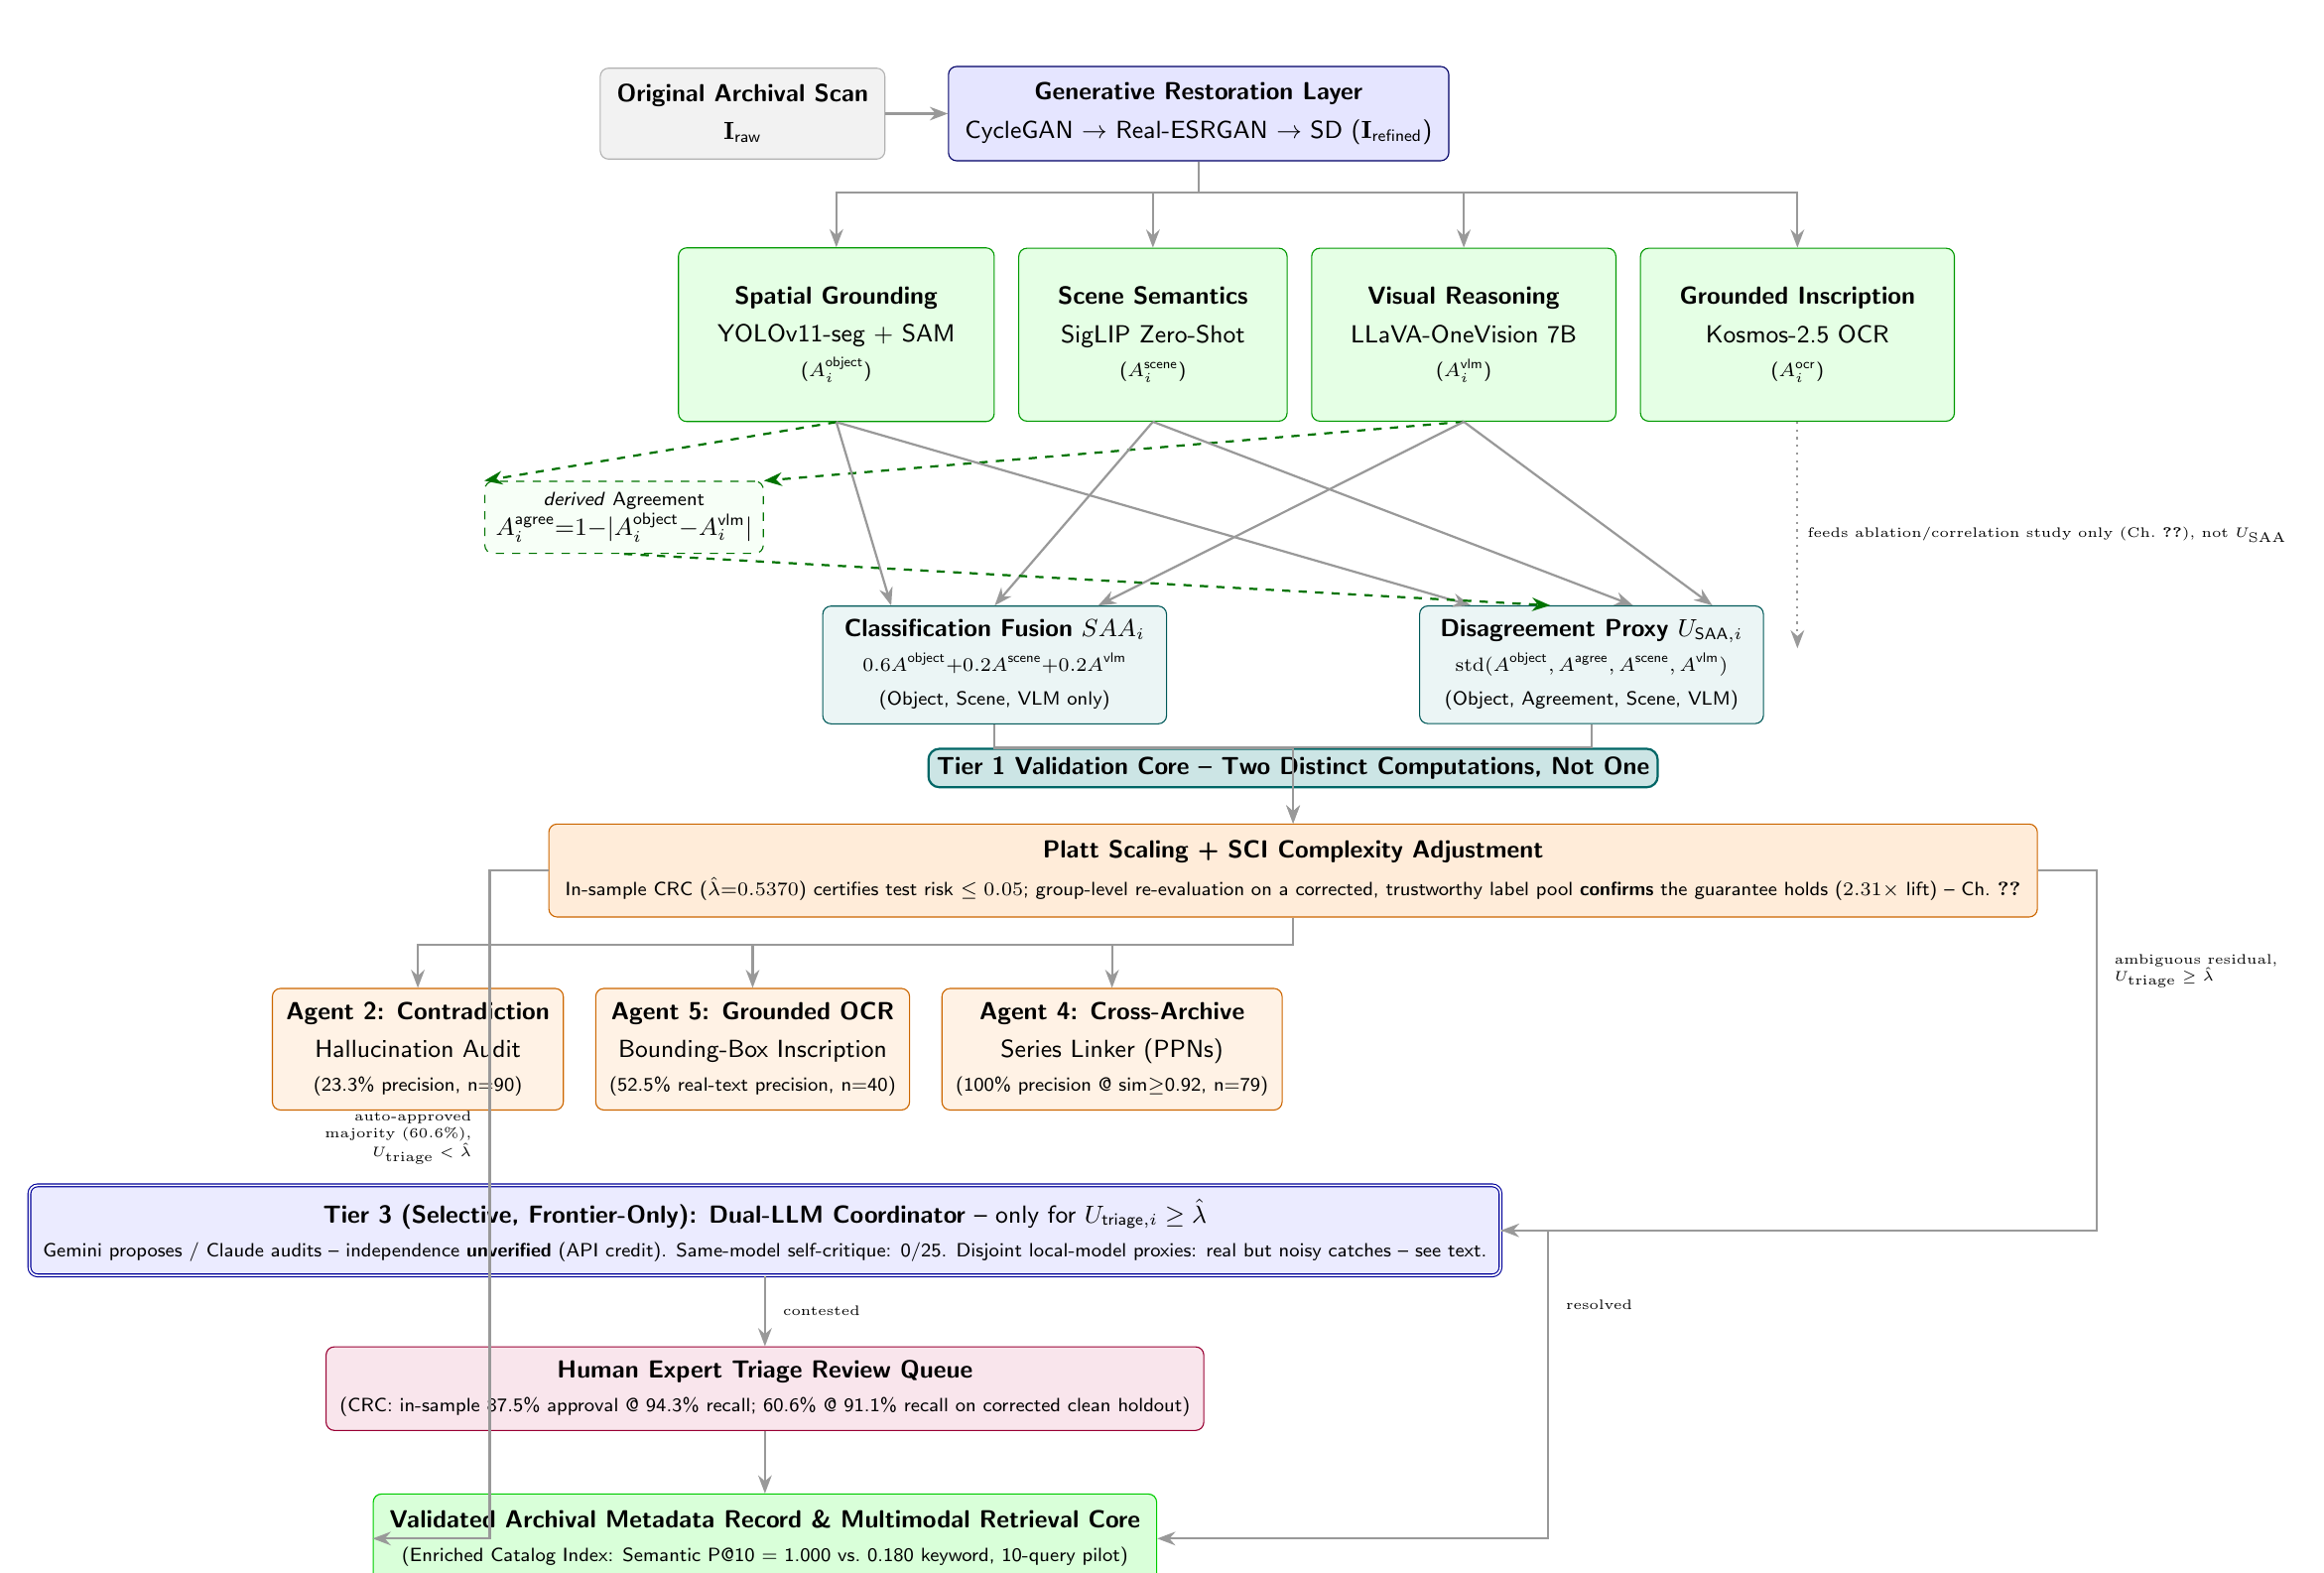
\begin{tikzpicture}[
    node distance=0.85cm and 0.3cm,
    font=\sffamily\small,
    box/.style={draw, rectangle, rounded corners=3pt, align=center, fill=blue!5, draw=blue!40!black, inner sep=6pt, minimum width=2.4cm, minimum height=1.0cm},
    agentbox/.style={draw, rectangle, rounded corners=3pt, align=center, fill=green!10, draw=green!60!black, inner sep=5mm, minimum width=2.6cm, minimum height=1.1cm},
    derivedbox/.style={draw, rectangle, dashed, rounded corners=3pt, align=center, fill=green!3, draw=green!45!black, inner sep=4pt, minimum width=2.2cm, minimum height=0.8cm},
    subcorebox/.style={draw, rectangle, rounded corners=3pt, align=center, fill=teal!8, draw=teal!70!black, inner sep=5pt, minimum width=4.4cm, minimum height=1.3cm},
    corelabel/.style={draw, rectangle, rounded corners=4pt, fill=teal!20, draw=teal!80!black, thick, inner sep=3pt},
    coordbox/.style={draw, rectangle, rounded corners=3pt, align=center, fill=blue!8, draw=blue!60!black, double, inner sep=5pt, minimum width=8.4cm, minimum height=1.0cm},
    curationbox/.style={draw, rectangle, rounded corners=3pt, align=center, fill=orange!10, draw=orange!80!black, inner sep=5pt, minimum width=2.6cm, minimum height=1.0cm},
    actionbox/.style={draw, rectangle, rounded corners=3pt, align=center, fill=purple!10, draw=purple!80!black, inner sep=5pt, minimum width=4.5cm, minimum height=0.9cm},
    arrow/.style={-Stealth, thick, draw=gray!80},
    derivedarrow/.style={-Stealth, thick, dashed, draw=green!45!black}
]

\node (raw) [box, fill=gray!10, draw=gray!60] {\textbf{Original Archival Scan}\\[1mm]$\mathbf{I}_{\text{raw}}$};
\node (resto) [box, right=0.8cm of raw, fill=blue!10] {\textbf{Generative Restoration Layer}\\[1mm]CycleGAN $\rightarrow$ Real-ESRGAN $\rightarrow$ SD ($\mathbf{I}_{\text{refined}}$)};

\node (a1) [agentbox, below left=1.1cm and -0.6cm of resto] {\textbf{Spatial Grounding}\\[1mm]YOLOv11-seg + SAM\\[0.5mm]{\scriptsize ($A_i^{\text{object}}$)}};
\node (a2) [agentbox, right=0.3cm of a1] {\textbf{Scene Semantics}\\[1mm]SigLIP Zero-Shot\\[0.5mm]{\scriptsize ($A_i^{\text{scene}}$)}};
\node (a3) [agentbox, right=0.3cm of a2] {\textbf{Visual Reasoning}\\[1mm]LLaVA-OneVision 7B\\[0.5mm]{\scriptsize ($A_i^{\text{vlm}}$)}};
\node (a4) [agentbox, right=0.3cm of a3] {\textbf{Grounded Inscription}\\[1mm]Kosmos-2.5 OCR\\[0.5mm]{\scriptsize ($A_i^{\text{ocr}}$)}};

\node (agree) [derivedbox, below=0.75cm of a1.south west, anchor=north east, xshift=1.1cm] {\scriptsize \textit{derived} Agreement\\$A_i^{\text{agree}}{=}1{-}|A_i^{\text{object}}{-}A_i^{\text{vlm}}|$};

\node (saabox) [subcorebox, below=2.35cm of $(a1.south)!0.5!(a2.south)$, anchor=north] {\textbf{Classification Fusion} $SAA_i$\\[0.5mm]{\scriptsize $0.6A^{\text{object}}{+}0.2A^{\text{scene}}{+}0.2A^{\text{vlm}}$}\\[0.5mm]{\scriptsize (Object, Scene, VLM only)}};
\node (usaabox) [subcorebox, below=2.35cm of $(a3.south)!0.5!(a4.south)$, anchor=north, xshift=-0.5cm] {\textbf{Disagreement Proxy} $U_{\text{SAA}, i}$\\[0.5mm]{\scriptsize $\operatorname{std}(A^{\text{object}}, A^{\text{agree}}, A^{\text{scene}}, A^{\text{vlm}})$}\\[0.5mm]{\scriptsize (Object, Agreement, Scene, VLM)}};

\node (corelabelnode) [corelabel, below=0.3cm of $(saabox.south)!0.5!(usaabox.south)$, minimum height=0.01cm] {\textbf{Tier 1 Validation Core -- Two Distinct Computations, Not One}};
\node (triage) [box, below=0.45cm of corelabelnode.south, fill=orange!15, draw=orange!80!black, minimum width=8.6cm] {\textbf{Platt Scaling + SCI Complexity Adjustment}\\[1mm]{\scriptsize In-sample CRC ($\hat{\lambda}{=}0.5370$) certifies test risk $\le 0.05$; group-level re-evaluation on a corrected, trustworthy label pool \textbf{confirms} the guarantee holds ($2.31\times$ lift) -- Ch.~\ref{ch:triage_risk_control}}};

\node (cur2) [curationbox, below left=0.9cm and -0.2cm of triage] {\textbf{Agent 2: Contradiction}\\[1mm]Hallucination Audit\\[0.5mm]{\scriptsize (23.3\% precision, n=90)}};
\node (cur5) [curationbox, right=0.4cm of cur2] {\textbf{Agent 5: Grounded OCR}\\[1mm]Bounding-Box Inscription\\[0.5mm]{\scriptsize (52.5\% real-text precision, n=40)}};
\node (cur4) [curationbox, right=0.4cm of cur5] {\textbf{Agent 4: Cross-Archive}\\[1mm]Series Linker (PPNs)\\[0.5mm]{\scriptsize (100\% precision @ sim$\ge$0.92, n=79)}};

\node (coord) [coordbox, below=0.95cm of $(cur2.south)!0.5!(cur4.south)$] {\textbf{Tier 3 (Selective, Frontier-Only): Dual-LLM Coordinator} -- only for $U_{\text{triage},i} \ge \hat\lambda$\\[0.5mm]{\scriptsize Gemini proposes / Claude audits -- independence \textbf{unverified} (API credit). Same-model self-critique: 0/25. Disjoint local-model proxies: real but noisy catches -- see text.}};

\node (hitl) [actionbox, below=0.9cm of coord] {\textbf{Human Expert Triage Review Queue}\\[0.5mm]{\scriptsize (CRC: in-sample 87.5\% approval @ 94.3\% recall; 60.6\% @ 91.1\% recall on corrected clean holdout)}};

\node (output) [box, below=0.8cm of hitl, fill=green!15, draw=green!80!black, minimum width=8.5cm] {\textbf{Validated Archival Metadata Record \& Multimodal Retrieval Core}\\[0.5mm]{\scriptsize (Enriched Catalog Index: Semantic P@10 = 1.000 vs.\ 0.180 keyword, 10-query pilot)}};

\draw [arrow] (raw) -- (resto);
\draw [arrow] (resto.south) -- ++(0,-0.4) -| (a1.north);
\draw [arrow] (resto.south) -- ++(0,-0.4) -| (a2.north);
\draw [arrow] (resto.south) -- ++(0,-0.4) -| (a3.north);
\draw [arrow] (resto.south) -- ++(0,-0.4) -| (a4.north);

\draw [derivedarrow] (a1.south) -- (agree.north west);
\draw [derivedarrow] (a3.south) -- (agree.north east);

\draw [arrow] (a1.south) -- ($(saabox.north west)!0.20!(saabox.north east)$);
\draw [arrow] (a2.south) -- ($(saabox.north west)!0.50!(saabox.north east)$);
\draw [arrow] (a3.south) -- ($(saabox.north west)!0.80!(saabox.north east)$);
\draw [arrow] (a1.south) -- ($(usaabox.north west)!0.15!(usaabox.north east)$);
\draw [derivedarrow] (agree.south) -- ($(usaabox.north west)!0.38!(usaabox.north east)$);
\draw [arrow] (a2.south) -- ($(usaabox.north west)!0.62!(usaabox.north east)$);
\draw [arrow] (a3.south) -- ($(usaabox.north west)!0.85!(usaabox.north east)$);
\draw [arrow, dotted] (a4.south) -- ++(0,-2.9) node[midway, right, font=\tiny] {feeds ablation/correlation study only (Ch.~\ref{ch:uncertainty_calibration}), not $U_{\text{SAA}}$};

\draw [arrow] (saabox.south) |- ($(saabox.south)+(0,-0.3)$) -| (triage.north);
\draw [arrow] (usaabox.south) |- ($(usaabox.south)+(0,-0.3)$) -| (triage.north);
\draw [arrow] (triage.south) -- ++(0,-0.35) -| (cur2.north);
\draw [arrow] (triage.south) -- ++(0,-0.35) -| (cur5.north);
\draw [arrow] (triage.south) -- ++(0,-0.35) -| (cur4.north);
\draw [arrow] (triage.east) -- ++(0.75,0) |- (coord.east)
  node[pos=0.14, right, font=\tiny, align=left, xshift=1mm] {ambiguous residual,\\$U_{\text{triage}} \ge \hat\lambda$};
\draw [arrow] (triage.west) -- ++(-0.75,0) |- (output.west)
  node[pos=0.20, left, font=\tiny, align=right, xshift=-1mm] {auto-approved\\majority ($60.6\%$),\\$U_{\text{triage}} < \hat\lambda$};

\draw [arrow] (coord.south) -- (hitl.north) node[midway, right, font=\tiny, xshift=1mm] {contested};
\draw [arrow] (coord.east) -- ++(0.6,0) |- (output.east) node[pos=0.12, right, font=\tiny, xshift=1mm] {resolved};

\draw [arrow] (hitl) -- (output);

\end{tikzpicture}%
}
\caption[Decoupled 3-Tier Dual-Core Validation and Multi-Agent Curation (DCV-MAC) Architecture]{Decoupled 3-Tier Dual-Core Validation and Multi-Agent Curation (DCV-MAC) Architecture. Tier 1's four models (solid green) feed \emph{two distinct} computations: the 3-term classification fusion $SAA_i$ and the 4-term disagreement proxy $U_{\text{SAA},i}$, which substitutes a derived Agreement signal (dashed, Object--VLM concordance) for OCR -- the two are related but not algebraically equivalent (Section~\ref{ch:methodology}). OCR separately feeds only the Tier~1 ablation/correlation study. Tier 3's Dual-LLM Coordinator is selective (triggered only above the disagreement threshold $\tau$) and frontier-only in deployment: a locally-reused same-model variant was tested and dropped after finding no verified value (0/25 self-flags); separate local tests with genuinely disjoint model pairs found real but individually-unreliable cross-model catches (Section~\ref{ch:methodology}), evidence for the architecture's rationale without yet replacing the deployed frontier pair. Tier 2 downstream curation agents process validated metadata post-hoc, per the Architectural Decoupling Rule.}
\label{fig:full_pipeline_flow}
\end{figure}

\begin{algorithm}[!htbp]
\caption{DCV-MAC Multi-Agent Validation Core and Triage Routing}
\label{alg:dcv_mac_triage}
\begin{algorithmic}[1]
\Require Archival image scan $\mathbf{I}_{\text{raw}}$, Tier 1 agent ensemble $\{M_{\text{object}}, M_{\text{scene}}, M_{\text{vlm}}, M_{\text{ocr}}\}$, fixed heuristic fusion weights $\mathbf{w} = [w_o, w_s, w_v]$ (the deployed weighting used for every empirical result in this thesis; see remark below), Platt calibration parameters $(A, B)$, Risk threshold $\hat{\lambda}$ from conformal calibration ($\hat{\lambda}=0.3720$ at $\alpha=0.05$ on the corrected, trustworthy group-level pool of Section~\ref{sec:clean_holdout}; the in-sample $C_1$ split of Section~\ref{ch:triage_risk_control} selected $\hat{\lambda}=0.5370$). (A separate Spatial Complexity Index estimator $\text{SCI}(\cdot)$ exists and feeds the distinct, non-deployed policy of Section~\ref{sec:complexity_triage}; it is not an input to this routing path.)
\Ensure Calibrated error probability $P(\text{error}_i)$, triage routing decision $d_i \in \{\text{Approve}, \text{Review}\}$, and enriched metadata record $\mathbf{M}_i$.
\State \textbf{Generative Preprocessing:} $\mathbf{I}_{\text{cyc}} \leftarrow \text{CycleGAN}(\mathbf{I}_{\text{raw}})$, \quad $\mathbf{I}_{\text{sr}} \leftarrow \text{RealESRGAN}(\mathbf{I}_{\text{cyc}})$
\State \quad $\mathbf{I}_{\text{refined}} \leftarrow \text{StableDiffusion}(\mathbf{I}_{\text{sr}}, \text{strength}=0.35)$
\State \textbf{Tier 1 Agent Ensemble Inference:}
\State \quad $A_i^{\text{object}} \leftarrow M_{\text{object}}(\mathbf{I}_{\text{refined}})$, \quad $A_i^{\text{scene}} \leftarrow M_{\text{scene}}(\mathbf{I}_{\text{refined}})$
\State \quad $A_i^{\text{vlm}} \leftarrow M_{\text{vlm}}(\mathbf{I}_{\text{refined}})$, \quad $A_i^{\text{ocr}} \leftarrow M_{\text{ocr}}(\mathbf{I}_{\text{refined}})$
\State \quad $A_i^{\text{agree}} \leftarrow 1 - |A_i^{\text{object}} - A_i^{\text{vlm}}|$ \Comment{derived pairwise concordance, not a fifth model}
\State \textbf{Heuristic Consensus Fusion:} $SAA_i \leftarrow w_o A_i^{\text{object}} + w_s A_i^{\text{scene}} + w_v A_i^{\text{vlm}}$
\State \textbf{Epistemic Uncertainty Calculation:} $U_{\text{SAA}, i} \leftarrow \operatorname{std}(A_i^{\text{object}}, A_i^{\text{agree}}, A_i^{\text{scene}}, A_i^{\text{vlm}})$
\State \textbf{Mean Core-Agent Confidence:} $\bar{c}_i \leftarrow \operatorname{mean}(A_i^{\text{object}}, A_i^{\text{agree}}, A_i^{\text{scene}}, A_i^{\text{vlm}})$
\State \textbf{Deployed Triage Score:} $U_{\text{triage}, i} \leftarrow 0.6 \cdot U_{\text{SAA}, i} + 0.4 \cdot (1 - \bar{c}_i)$ \Comment{$\hat\lambda$ is calibrated against this quantity, not the SCI-based variant of Section~\ref{sec:complexity_triage}}
\State \textbf{Platt Scaling Calibration:} $P(\text{error}_i) \leftarrow \frac{1}{1 + \exp(A \cdot SAA_i + B)}$
\State \textbf{Tier 2 Downstream Curation} \Comment{runs on \emph{every} validated image, independent of $d_i$}
\State \quad $\mathbf{M}_i^{\text{contradiction}} \leftarrow \text{Agent2\_Contradiction}(A_i^{\text{object}}, A_i^{\text{vlm}})$
\State \quad $\mathbf{M}_i^{\text{linker}} \leftarrow \text{Agent4\_CrossArchiveLinker}(\mathbf{I}_{\text{refined}})$
\State \quad $\mathbf{M}_i^{\text{ocr}} \leftarrow \text{Agent5\_GroundedOCR}(A_i^{\text{ocr}})$
\State $\mathbf{M}_i \leftarrow \mathbf{M}_i^{\text{consensus}} \cup \mathbf{M}_i^{\text{contradiction}} \cup \mathbf{M}_i^{\text{linker}} \cup \mathbf{M}_i^{\text{ocr}}$
\If{$U_{\text{triage}, i} \ge \hat{\lambda}$}
    \State $d_i \leftarrow \text{Review}$
    \State \textbf{Tier 3 (selective, frontier-only):} escalate only this residual --- Gemini proposes, Claude audits
    \State \quad unresolved cases route to the Human Expert Review Queue
\Else
    \State \textbf{Automatic Approval:} $d_i \leftarrow \text{Approve}$
\EndIf
\State \Return $(P(\text{error}_i), d_i, \mathbf{M}_i)$
\end{algorithmic}
\end{algorithm}

\section{Generative Restoration Layer and Methodological Discipline}
Archival scans exhibit severe chemical decay, film grain, and fading. Before feature extraction, Tier 1 normalizes raw grayscale scans ($\mathbf{I}_{\text{raw}}$) into a modern visual regime ($\mathbf{I}_{\text{refined}}$) using a three-stage generative pipeline: CycleGAN domain translation \cite{cyclegan2017} $\rightarrow$ Real-ESRGAN $4\times$ super-resolution \cite{realesrgan2021} $\rightarrow$ Stable Diffusion Img2Img refinement \cite{stable_diffusion2022} ($\text{strength}=0.35$).

\begin{flushleft}
\textbf{The Axiom of Archival Integrity}: The AI-restored image ($\mathbf{I}_{\text{refined}}$) is strictly an internal visual token translation layer generated for model feature alignment. It is NEVER stored or presented as primary historical evidence. All catalog metadata is anchored strictly back to original digitized scans ($\mathbf{I}_{\text{raw}}$).
\end{flushleft}

Decoupling generative restoration to the input feature layer yields a $+0.052$ mAP object detection gain (measured end-to-end: the full 3-stage pipeline's output vs.\ the same detector on raw scans, same image set; individual restoration stages were not separately ablated) while protecting primary catalog records from generative hallucinations. A per-image Laplacian-variance sharpness measurement (raw scan vs.\ the same image's full-pipeline restored output, across the manifest's full image set) shows generative translation increases structural edge sharpness in $83.8\%$ of scans.

\begin{figure}[!htbp]
\centering
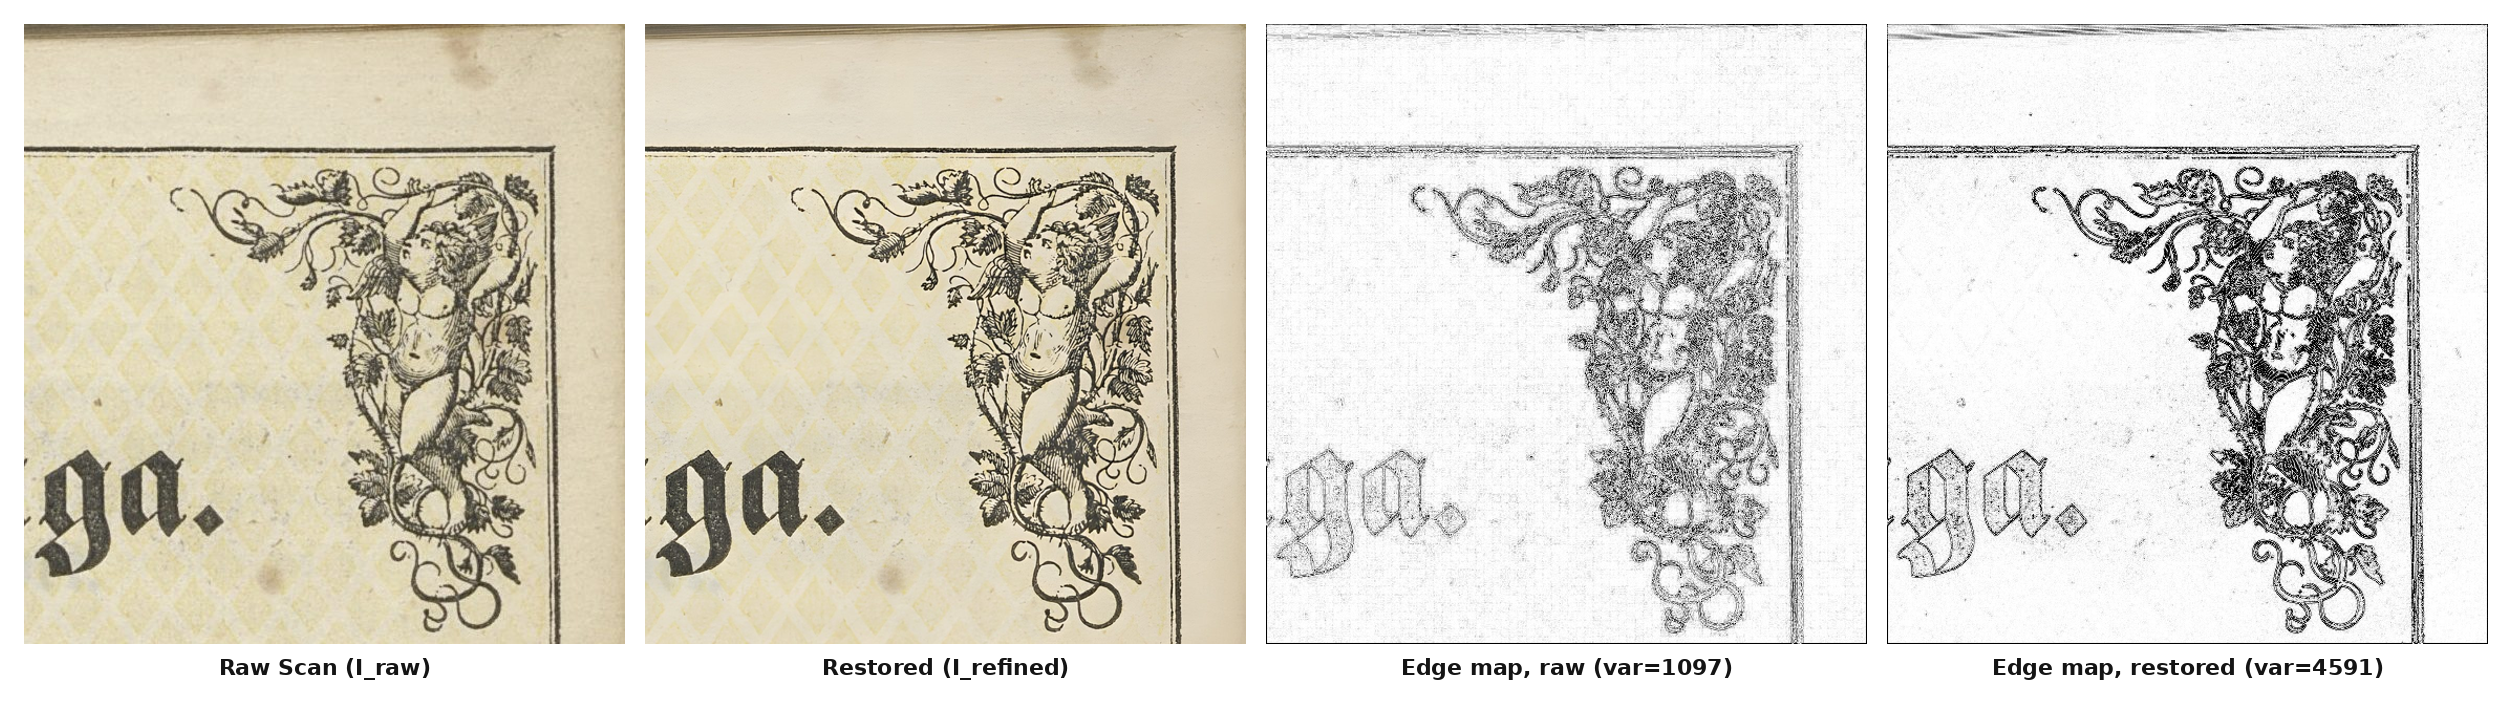
\includegraphics[width=\textwidth]{restoration_comparison_labeled.png}
\caption[Generative Restoration Pipeline, Input vs.\ Output]{Generative Restoration Pipeline, Input vs.\ Output. The full three-stage pipeline (CycleGAN domain translation $\to$ Real-ESRGAN $4\times$ super-resolution $\to$ Stable Diffusion Img2Img refinement, strength$=0.35$) maps a raw scan ($\mathbf{I}_{\text{raw}}$, left) to a normalized visual feature representation ($\mathbf{I}_{\text{refined}}$, second panel). Because the pipeline is deliberately restrained (a low diffusion strength, chosen specifically to avoid hallucinating content not in the original), the visual difference is subtle to the eye at a glance -- the right two panels make it explicit: Laplacian edge-response maps of the same crop, with the measured edge variance printed on each. For this example, structural edge variance increases from $1{,}097$ (raw) to $4{,}591$ (restored), a $4.2\times$ gain, consistent with the population-level finding above that restoration increases measured sharpness on $83.8\%$ of scans (Figure~\ref{fig:generative_restoration_triptych}).}
\label{fig:generative_restoration_triptych}
\end{figure}

\section{Canonical Formulation of Scene-Aware Agreement (SAA)}
\label{sec:canonical_saa}
These four quantities are \emph{not} four stages of one computation: Levels 2, 3 and 4 are three different scalars, built from overlapping subsets of the same agent outputs, for three different purposes -- classification, uncertainty, and routing. The numbering is a naming convention, not a pipeline order. Because several other quantities in this thesis draw on different subsets again, Table~\ref{tab:signal_sets} states every signal set in one place; any reference to ``the agents'' below should be read against it.

\begin{table}[!htbp]
\centering
\caption[Every agent-signal set used in this thesis and the quantity each]{Every agent-signal set used in this thesis and the quantity each defines. \emph{Ag} denotes the derived Agreement signal $1-|A^{\text{object}}-A^{\text{vlm}}|$, which is not an independent model. The sets differ for defensible reasons -- classification, disagreement, architectural ablation and meta-classification are different questions -- but they are easy to conflate, and one of this thesis's own errors arose from exactly that (Section~\ref{sec:signal_decomposition}).}
\label{tab:signal_sets}
\small
\begin{tabular}{p{4.3cm}p{4.3cm}cp{3.3cm}}
\toprule
\textbf{Quantity} & \textbf{Signals} & \textbf{$k$} & \textbf{Where used} \\
\midrule
$SAA_i$ -- classification fusion (Level 2) & Object, Scene, VLM & 3 & Scene prediction; error label for the corrected held-out evaluation \\
\texttt{comparison\_fusion\_score} -- stored fusion column & Object, \emph{Ag}, Scene, VLM & 4 & Error label for the in-sample $C_1$ result and all CRC experiments \\
$U_{\text{SAA},i}$ -- disagreement proxy (Level 3) & Object, \emph{Ag}, Scene, VLM & 4 & Every headline uncertainty figure \\
$U_{\text{triage},i}$ -- routing score (Level 4) & $U_{\text{SAA}}$ and $\bar{c}$, same 4 signals & 4 & Auto-approval decision against $\hat\lambda$ \\
$\sigma_{\text{model}}$ -- architectural ablation & Object, Scene, VLM, OCR & 4 & Tier 1 leave-one-out complementarity \\
AWLF v2 meta-features (Algorithm~\ref{alg:awlf_v2}) & Object, \emph{Ag}, Scene, VLM, Restoration, OCR & 6 & Supervised error meta-classifier \\
Deep-ensemble baseline & the same 6 & 6 & Baseline in the held-out comparison \\
Shapley coalition (Appendix~\ref{app:shapley}) & Object, \emph{Ag}, Scene, VLM & 4 & Interpretability only; not a production weighting \\
\bottomrule
\end{tabular}
\end{table}

\begin{enumerate}
    \item \textbf{Level 1 (Agent Output Vector)}: For an image $i$, the Tier 1 agents produce four signals in $[0,1]$ -- spatial object grounding $A_i^{\text{object}}$, zero-shot scene $A_i^{\text{scene}}$, VLM description $A_i^{\text{vlm}}$, and grounded inscription $A_i^{\text{ocr}}$. Two of the four are \emph{saturating counts} rather than model confidences, and stating the actual constructions matters for how the spread over them should be read:
\begin{equation*}
\begin{aligned}
A_i^{\text{object}} &= \min\!\left(\tfrac{\text{VQA object count}}{3},\, 1\right) && \in \{0,\tfrac13,\tfrac23,1\} \\
A_i^{\text{scene}}  &= \text{VQA scene confidence, clipped to } [0,1] && \in \{0.5,\,1\} \text{ in practice} \\
A_i^{\text{vlm}}    &= \text{VQA object-presence score} && \in \{0,1\} \\
A_i^{\text{ocr}}    &= \min\!\left(\tfrac{\text{characters of Kosmos-2.5 output}}{80},\, 1\right) &&
\end{aligned}
\end{equation*}
$A_i^{\text{ocr}}$ is therefore a measure of \emph{how much} text the OCR model emitted, not of how confident or correct that text is -- a distinction that matters given Section~\ref{sec:agent5_ocr}'s finding that $47.5\%$ of the ``candidate real OCR'' bucket contains no legible text at all, the model having produced fluent but fabricated markdown. A length-based signal scores such output high. $A_i^{\text{ocr}}$ does not enter $SAA$, $U_{\text{SAA}}$ or the triage score; it participates only in the model-level ablation of Section~\ref{ch:uncertainty_calibration}, the AWLF feature vector (Algorithm~\ref{alg:awlf_v2}), the six-agent deep-ensemble baseline, and the pairwise correlation matrix. \paragraph{A provenance correction: the object signal is not the detector's box count.} An audit of the stored agent table established that $A_i^{\text{object}}$ was not produced by the Spatial Grounding Agent, as an earlier version of this thesis stated. The distilled student's box count is zero for all $12{,}110$ images, so the intended path never executed and a fallback supplied the VQA object count instead: $A_i^{\text{object}} = \min(\text{VQA object count}/3,\,1)$ reproduces the deployed column exactly on every image. Because $A_i^{\text{vlm}}$ is the VQA object-presence score, the two signals share one source, which is why $A_i^{\text{vlm}} = \mathbb{I}[A_i^{\text{object}} > 0]$ holds with no exceptions corpus-wide (Section~\ref{sec:signal_decomposition}). The deployed Tier 1 vector therefore contains three separately-measured quantities, not four. Every number in this thesis was computed from the table as it stands and is unaffected; what changes is the description of one input and the explanation of the redundancy analysed in Section~\ref{sec:signal_decomposition}. Section~\ref{sec:signal_rebuild} reports a reconstruction of the signals from the raw model outputs, and the retest that followed.

\paragraph{Verified by execution, not by inspection}: The audit above reads the stored table and infers which code path produced it. That inference was subsequently confirmed by re-running the fusion stage over the whole corpus, twice, along the two routes actually available. Pointed at the live project tree, where the spatial detector's aligned detections, the v8 agreement scores and the CLIP/SigLIP scene labels are absent, the stage takes its documented manifest fallback and regenerates the committed $12{,}110$-row table \emph{exactly}: all five columns identical on every row, maximum absolute difference $0$. Pointed instead at the archived tree where those three files do exist, it does not --- $A^{\text{object}}$ agrees on $11.6\%$ of images, $A^{\text{scene}}$ on none.

That asymmetry is not a contest between two versions of the data. The archived model outputs cover $231$, $230$ and $231$ images respectively, out of $12{,}110$; they cannot populate a corpus-wide table at all. Together with \texttt{student\_v3\_count} being non-zero on \emph{none} of the $12{,}110$ manifest rows, this places the fallback in control of roughly $98\%$ of the corpus, and settles by execution what the audit had established by inspection.

Two things follow, and they point in opposite directions. The pipeline is reproducible end to end: the table underpinning every result here regenerates bit-for-bit from its source files, which is a stronger reproducibility position than most work of this kind can claim, and it can be re-checked with one command. But what it reproduces is a corpus-wide signal set of which only the vision-language and OCR components ever ran corpus-wide. The spatial detector and the scene classifier were executed on under $2\%$ of the archive, and the remainder was filled by a fallback derived from the VQA answer. A genuinely four-model run over all $12{,}110$ images has since been completed, and is reported next.

\paragraph{A real detector, run on every image}: The spatial detector was the one Tier~1 model without corpus-wide inference, and it is the signal the fallback replaced, so the standing objection to this thesis's negative result is that fixing the provenance would rescue it. That objection is now testable. The trained YOLOv11m archival-taxonomy detector was executed over all $12{,}110$ images ($12.4$ minutes on one GPU, mean $1.73$ boxes per image, no detections on $2{,}882$). One caveat belongs up front: the distilled \texttt{student\_iter\_3} checkpoint is no longer on disk, so this is a genuine archival-taxonomy detector and not a reconstruction of the historical student, and no claim is made that its classification quality matches one tuned for the deployed pipeline.

The provenance defect was material. The real object signal correlates with the deployed one at only $r=0.59$, the two agree exactly on $25.7\%$ of images and on the binary presence call for $76.6\%$, and the detector finds nothing on $2{,}882$ images against the fallback's $1{,}403$. Most importantly the perfect dependency breaks: $A^{\text{vlm}} = \mathbb{I}[A^{\text{object}}>0]$ holds on $100\%$ of images under the fallback and on $76.6\%$ under the real detector, so $A^{\text{agree}}$ becomes a genuine comparison of two independently measured quantities rather than an algebraic restatement of one.

It does not rescue the claim. On the corrected held-out partition the rebuilt signal gives disagreement $\text{ROC-AUC}=0.8304$ against a confidence baseline of $0.8674$: still behind. The difference, $-0.037$ with $95\%$ CI $[-0.087, 0.012]$, now spans zero, which is weaker evidence than the deployed comparison rather than stronger --- at $n=249$ this retest is underpowered, and that is the honest description of it. What can be said is that the negative result survives replacing the fallback with real corpus-wide inference, which is the specific objection it was run to answer.

A third variant, removing the $\min(\text{count}/3, 1)$ saturation so the object signal is continuous, is reported in the accompanying record but must not be read as a disagreement win. Its classifier errs on $82\%$ of the test partition, because scaling the box count by the corpus maximum puts nearly every image below the $0.5$ threshold; the confidence baseline falls below chance for the same reason, which is what makes disagreement appear to overtake it. It is an artifact of a broken classifier, and is retained only to document that the saturation cannot simply be removed without redesigning the threshold.

\paragraph{The complete Tier 1 re-run}: The detector run above was subsequently extended to the whole ensemble. All four Tier~1 models --- YOLOv11 detection, SigLIP scene classification, LLaVA-OneVision VQA and Kosmos-2.5 grounded OCR --- were executed over all $12{,}110$ corpus images, taking $4$ hours $38$ minutes across four RTX~A6000s. This is the first genuinely four-model corpus-wide inference run in the project: previously only the vision-language and OCR components had corpus coverage, and every other signal was either a manifest fallback or measured on $231$ images.

The run exposed a second degeneracy, independent of the object fallback and invisible until the model actually ran. The deployed $A^{\text{vlm}}$ is the fraction of the four VQA questions answered ``substantively'', operationalised as at least three words. On real LLaVA output the first two questions are descriptive and answered substantively on $100\%$ and $99.9\%$ of images, while the third and fourth are yes/no and answered in a single word on $100\%$ and $99\%$. The fraction is therefore $2/4$ on $\mathbf{98.9\%}$ of the corpus. The deployed VLM signal encodes the \emph{question format} rather than the image, and cannot contribute to a disagreement statistic because it barely varies. The answers themselves do carry signal --- the presence question splits $7{,}183$ affirmative against $4{,}924$ negative --- so the rebuild reads the answers rather than counting their words.

Rebuilt on genuinely measured signals throughout, the discretisation that Section~\ref{sec:formulation_search} rests on disappears: $A^{\text{scene}}$ becomes continuous with $11{,}882$ distinct values and $U_{\text{SAA}}$ takes $\mathbf{11{,}786}$ distinct values in place of eight. The dependency loosens correspondingly, $A^{\text{vlm}} = \mathbb{I}[A^{\text{object}}>0]$ falling from $100\%$ to $78.9\%$ of images.

The conclusion does not move. On the corrected held-out partition the rebuilt disagreement signal scores $\text{ROC-AUC} = 0.8098$ against a confidence baseline of $0.8483$, a difference of $-0.039$ with $95\%$ CI $[-0.083, 0.005]$. Disagreement remains behind confidence when every signal entering it has been measured by a real model on every image, when the derived term is a genuine comparison, and when the eight-value discretisation is gone. One caveat limits the weight this can bear: the rebuilt fusion errs on $43.4\%$ of the test partition against the deployed $28.1\%$, so it is a worse classifier, and part of the gap may reflect that rather than the uncertainty signal. The honest summary is that the central negative result survives the most complete test available to this thesis, and that the test is not decisive on its own.

\paragraph{The experiments that consume these signals, recomputed}: Several published
experiments were computed on the deployed signal set and had not been revisited. Those that
actually consume the four agent scalars were recomputed on the rebuilt ones, with the error label
re-derived at a threshold refitted on the calibration partition. Conformal risk control is
recomputed separately with its own recalibration, and the Exp~31 spatial meta-learner operates on
box-level IoU rather than these scalars and is unaffected.

Two results are stable and one is not. AWLF v2 is essentially unchanged, $0.8685$ deployed against
$0.8722$ rebuilt, although the comparison is not quite like-for-like: the deployed feature vector
includes a restoration-agent column the re-run does not reproduce, so the rebuilt model works from
five features rather than six. The Tier~1 ablation keeps its shape, with the object signal
load-bearing under both.

The Shapley attribution does not survive. Computed over the same coalition with the same value
function, the deployed and rebuilt attributions differ substantially:

\begin{center}
\small
\begin{tabular}{@{}l r r@{}}
\toprule
\textbf{Agent} & \textbf{Deployed $\phi$} & \textbf{Rebuilt $\phi$} \\
\midrule
Object & $0.1482$ & $0.1482$ \\
Agreement & $0.0857$ & $0.0622$ \\
Scene & $0.0843$ & $\mathbf{0.0249}$ \\
VLM & $0.0459$ & $\mathbf{0.1329}$ \\
\bottomrule
\end{tabular}
\end{center}

The vision-language agent's attribution nearly triples and the scene agent's falls to a third. The
direction is what the provenance work predicts: the deployed $A^{\text{vlm}}$ was $2/4$ on $98.9\%$
of images and could contribute almost nothing, so the coalition assigned its share elsewhere. Once
the signal carries content, it is the second most important member. The same reversal appears in
the ablation --- on deployed signals, removing the VLM term \emph{improved} the fitted score by
$0.0108$; on rebuilt signals, removing it \emph{costs} $0.043$. The published attribution in
Appendix~\ref{app:shapley} should therefore be read as an attribution over the deployed signal set
specifically, and not as a statement about the agents themselves.

\paragraph{Redesigning the signals to use what the models emit}: The reductions of
Section~\ref{sec:canonical_saa} discard most of each model's output --- a saturating count where
the detector produced confidences and locations, a binary flag where the classifier produced a
distribution over five categories, one bit where the vision-language model produced a paragraph.
It is therefore fair to ask whether the negative result is a property of \emph{disagreement} or of
the \emph{reduction}. Each signal was rebuilt from its model's own output to find out:
$A^{\text{object}}$ as the detector's maximum box confidence, $A^{\text{scene}}$ as either the
maximum softmax over the five categories or the classifier's peakedness $1-H/\log 5$,
$A^{\text{vlm}}$ as the fraction of the ten taxonomy classes the model names, and
$A^{\text{agree}}$ as a comparison of two now-independent measurements. Each variant received its
own decision threshold, refitted on the calibration partition.

The signals become incomparably richer. $A^{\text{object}}$ goes from $4$ distinct values to
$8{,}979$, $A^{\text{scene}}$ from $2$ to $11{,}882$, and $U_{\text{SAA}}$ from $8$ to $1{,}247$ on
the labelled pool. The eight-cell structure, and with it the ceiling of
Section~\ref{sec:formulation_search}, disappears entirely.

The claim fails harder.

\begin{table}[!htbp]
\centering
\caption[Disagreement against confidence on redesigned signals]{Disagreement against a plain confidence baseline on the corrected test partition, with the signals rebuilt from each model's own output. Each variant has its own decision threshold fitted on calibration, so the error labels differ between rows; the comparison to read is within a row.}
\label{tab:redesigned_signals}
\small
\begin{tabular}{@{}l c c c c@{}}
\toprule
\textbf{Signal set} & \textbf{bal.\ acc} & \textbf{$U_{\text{SAA}}$ values} & \textbf{disagreement} & \textbf{confidence} \\
\midrule
Deployed & $0.7802$ & $8$ & $0.8600$ & $0.8828$ \\
Redesigned, max softmax & $0.6625$ & $1{,}247$ & $0.5547$ & $\mathbf{0.8324}$ \\
Redesigned, peakedness & $0.6825$ & $1{,}247$ & $0.6273$ & $\mathbf{0.8430}$ \\
\bottomrule
\end{tabular}
\end{table}

On the deployed signals disagreement trails confidence by $0.023$, a margin small enough that the
chapter's argument had to lean on the ceiling to close it. On the redesigned signals it trails by
$\mathbf{0.278}$ and $\mathbf{0.216}$, with $95\%$ intervals of $[-0.357, -0.202]$ and
$[-0.293, -0.135]$ --- both lying entirely below zero. Giving every signal its full resolution does
not rescue disagreement; it separates confidence from it decisively. The reason is visible in the
columns: as the signals gain resolution the confidence baseline improves to $0.83$--$0.84$ while
the spread falls towards chance, because a richer $SAA$ is a better direct estimate of whether the
pipeline is right, and its spread is not.

Two cautions belong with this. The redesigned classifier is worse in balanced accuracy than the
deployed one ($0.66$--$0.68$ against $0.78$), so this is not a proposal to deploy; it is a test of
where the negative result comes from. And an intermediate version of this experiment selected its
threshold by raw error rate and reported an apparent halving of the error rate to $0.1526$. That
figure is exactly the majority-class rate on an $84.7\%$-positive partition, and the rule behind it
predicted scene-present on $100\%$ of images --- the AWLF v1 pathology of Section~\ref{sec:awlf}
recurring for the third time in this thesis. It is recorded because the objective, not the signals,
produced it.

\paragraph{Carrying the re-run through Tier 2 and Tier 3}: The rebuilt Tier~1 signals were fed
onward through the rest of the architecture. Tier~2's contradiction agent is directly computable
from them --- it flags an image when the vision-language model names a taxonomy object the detector
did not return --- and on the full corpus it fires on $71.97\%$ of images, $14{,}933$ flags in
total. That rate is dominated by taxonomy mismatch rather than by hallucination: the detector
recognises ten classes while the VLM describes freely, so \emph{clothing} ($4{,}821$), \emph{text}
($2{,}135$) and \emph{tree} ($2{,}076$) alone account for most of it. This is consistent with
Section~\ref{sec:agent2_contradiction}'s gold labelling, which found only $23.3\%$ of $101$ such
candidates were genuine hallucinations and the remainder detector misses; the corpus figure is a
candidate rate, not an error rate.

The instructive result is where those flags fall relative to the routing decision. Routing on the
deployed signals sends $3{,}620$ images onward and clears $8{,}490$; routing on the rebuilt signals
sends $5{,}236$ and clears $6{,}874$. Under either, the contradiction flag is \emph{more} common
among the automatically approved images than among the escalated ones --- $85.0\%$ against $41.4\%$
on deployed signals, $85.9\%$ against $53.7\%$ on rebuilt. The images the uncertainty score trusts
most are the ones Tier~2 most often finds a VLM-detector disagreement on.

This is the Architectural Decoupling Rule behaving exactly as specified: Tier~2 runs on
post-validation metadata, after routing, and cannot influence it. But the consequence deserves
stating plainly, because the architecture's rationale implies the opposite would be reassuring.
Tier~2 supplies no corroboration for the triage decision. A curator reviewing the auto-approved
pile would find contradiction flags on most of it, and those flags carry no weight in whether the
image was auto-approved in the first place. Whether that independence is a virtue --- enrichment
kept cleanly separate from trust --- or a missed signal is a design question this thesis does not
settle, and it could not have been asked before the models were run corpus-wide.

Tier~3 could not be executed. The deployed coordinator pairs Gemini~2.5~Flash with
Claude~3.5~Sonnet and requires paid frontier API credit, which this project does not have;
Section~\ref{ch:methodology} records it as untested rather than falsified, and that remains the
position. What the re-run does supply is the exact load it would receive: $3{,}620$ images at the
deployed operating point, $5{,}236$ on rebuilt signals. 

\paragraph{Agent 4, recomputed corpus-wide}: Cross-archive linking was the one Tier~2 agent the
re-run could not initially reach, because the corpus SigLIP pass stored the five scene-category
probabilities rather than the embedding vectors. A second pass stored the embeddings for all
$12{,}110$ images, and nearest-neighbour search restricted to \emph{different} publication volumes
was run over the $1{,}722$ volumes in the corpus. The deployed benchmark of
Section~\ref{sec:agent4_linking} ran on a sample; this is the full archive.

The nearest cross-volume neighbour has median cosine similarity $0.850$ and mean $0.855$, which is
itself informative: in an archive of nineteenth-century engravings almost every image has a fairly
similar counterpart somewhere else, because the embedding is dominated by style and medium rather
than by composition. Selectivity therefore depends entirely on where the threshold is placed. At
the $0.92$ cut-off where Section~\ref{sec:agent4_linking}'s gold labelling found precision
reaching $100\%$ on $79$ sampled pairs, $2{,}434$ images ($20.1\%$ of the corpus) have a candidate
link; at $0.95$ that falls to $1{,}052$ and at $0.98$ to $96$. The highest-scoring pairs reach
similarity $1.000$ and are genuine duplicate plates appearing in two separately catalogued
volumes, which is the intended use case.

Two cautions belong with these counts. The gold labels cover the pairs sampled in
Section~\ref{sec:agent4_linking}, not these, so the bands above are volumes of \emph{candidates}
rather than verified links; extrapolating the sampled precision to $2{,}434$ corpus pairs assumes a
transfer that has not been tested. And a mean nearest-neighbour similarity of $0.855$ means the
$0.92$ threshold sits well inside the bulk of the distribution rather than in its tail, so the
operating point is sensitive to small changes in it.

\paragraph{The rebuilt pipeline run end to end, calibrated on its own signals}: Applying the
deployed conformal threshold to a rebuilt triage score is not a deployment, because $\hat\lambda$
is calibrated against a particular score. The rebuilt pipeline was therefore recalibrated
throughout --- decision threshold and conformal threshold both fitted on the calibration
partition, with the test partition never consulted --- so that it is evaluated as a system rather
than as a component swapped into someone else's settings.

That distinction turned out to matter more than any other choice in this section. Inheriting the
deployed $0.5$ decision threshold, the rebuilt classifier errs on $43.4\%$ of the test partition
and its risk bound fails at three of five risk levels, which would invite the conclusion that real
signals perform worse than the fallback. They do not. The $0.5$ threshold belongs to the deployed
signal scales, and the rebuilt signals sit differently --- $A^{\text{scene}}$ alone has mean
$0.81$. Retuning the threshold on the calibration partition alone moves the test error rate from
$43.4\%$ to $\mathbf{27.7\%}$, against $22.5\%$ for the deployed pipeline, and the two signal sets
rank scene presence almost identically ($\text{ROC-AUC}$ $0.7624$ rebuilt against $0.7789$
deployed). Nearly all of the apparent degradation was an untuned hyperparameter.

Recalibrated, the rebuilt pipeline satisfies the risk bound at four of the five levels tested,
including the deployed operating point.

\begin{table}[!htbp]
\centering
\caption[Deployed and rebuilt pipelines end to end]{The two pipelines end to end on the corrected PPN-disjoint test partition ($n=249$), each with its own conformal calibration. The rebuilt pipeline uses signals measured by all four models on all $12{,}110$ images.}
\label{tab:end_to_end}
\small
\begin{tabular}{@{}l cc cc@{}}
\toprule
& \multicolumn{2}{c}{\textbf{Deployed}} & \multicolumn{2}{c}{\textbf{Rebuilt}} \\
\cmidrule(lr){2-3}\cmidrule(lr){4-5}
$\alpha$ & auto-approval & recall & auto-approval & recall \\
\midrule
$0.01$ & $30.9\%$ & $96.4\%$ & $21.7\%$ & $100.0\%$ \\
$0.02$ & $36.6\%$ & $94.6\%$ & $37.8\%$ & $98.6\%$ \\
$\mathbf{0.05}$ & $\mathbf{60.6\%}$ & $\mathbf{91.1\%}$ & $\mathbf{55.8\%}$ & $\mathbf{84.1\%}$ \\
$0.10$ & $60.6\%$ & $91.1\%$ & \emph{bound not met} & --- \\
$0.15$ & $81.5\%$ & $57.1\%$ & $76.3\%$ & $50.7\%$ \\
\bottomrule
\end{tabular}
\end{table}

At $\alpha=0.05$ the rebuilt pipeline certifies $55.8\%$ automatic approval at $84.1\%$ error
recall, with empirical test risk $0.044$ inside the bound, against the deployed $60.6\%$ and
$91.1\%$. It is a somewhat less efficient system built on honestly measured signals rather than a
markedly worse one. The exception is $\alpha=0.10$, where empirical risk reaches $0.112$ and the
bound is missed on this partition; conformal risk control bounds risk in expectation over the
calibration draw rather than on every realisation, so a single exceedance is not a refutation, but
it is reported rather than omitted.

\paragraph{What this costs at archive scale}: The throughput measured during the corpus run
projects directly. On the same four GPUs, a $53{,}000$-image archive would take approximately
$0.9$ hours for detection, $2.2$ for scene classification, $5.8$ for the vision-language model and
$11.9$ for grounded OCR: about $\mathbf{21}$ hours in total, producing roughly $36$\,MB of signal
output. Inference is not the constraint. The constraint is that running the archive end to end
produces a decision for every image and a measurement of correctness for none of them: there are
$1{,}535$ human labels for $12{,}110$ images and none at all for the further $40{,}890$ a
$53{,}000$-image archive would add. Scaling the compute multiplies the output; it does not
multiply the evidence, and the certified figures above would still rest on the same $249$ labelled
test images.

A fifth signal, \textit{Agreement}, is \emph{derived} rather than measured:
    \begin{equation}
        A_i^{\text{agree}} = 1 - \left|A_i^{\text{object}} - A_i^{\text{vlm}}\right|
        \label{eq:agree}
    \end{equation}
    It quantifies concordance between the spatial and VQA agents specifically. It is not a fifth model, and Caution 1 below explains why its derived status matters.

    \item \textbf{Level 2 (Scene-Aware Agreement Score)}: The classification fusion score $SAA_i$ predicts scene presence, and thresholding it at $0.5$ against the human label is what defines the ``error'' target that every uncertainty evaluation in this thesis is scored against. It is a weighted linear combination over three agents:
    \begin{equation}
        SAA_i = w_o A_i^{\text{object}} + w_s A_i^{\text{scene}} + w_v A_i^{\text{vlm}},
        \qquad w_o = 0.6,\; w_s = 0.2,\; w_v = 0.2
    \end{equation}
    Caution 2 below records an important qualification: a second fusion column exists in the pipeline, and it -- not this one -- defines the error label behind two of the thesis's headline numbers.

    \item \textbf{Level 3 (Disagreement Uncertainty Proxy)}: Level 2 answers \emph{what} is in the image; Level 3 answers \emph{how much the agents disagree about it}, and is the quantity every headline error-detection figure in this thesis is computed from. The two are separate by construction -- a weighted mean over three signals versus a spread over four -- so $U_{\text{SAA},i}$ is not a rescaling of $SAA_i$ and in particular $U_{\text{SAA},i} \ne 1 - SAA_i$:
    \begin{equation}
        U_{\text{SAA}, i} = \operatorname{std}\left(A_i^{\text{object}},\ A_i^{\text{agree}},\ A_i^{\text{scene}},\ A_i^{\text{vlm}}\right)
    \end{equation}
    Cautions 1 and 3 below apply to this definition.

    \item \textbf{Level 4 (Operational Triage Score)}: This thesis defines two triage scores sharing the same $0.6/0.4$ structural form but built from different second terms. Only one is the quantity Algorithm~\ref{alg:dcv_mac_triage} and the deployed conformal threshold $\hat\lambda$ actually use.
    \begin{itemize}
        \item \emph{SCI-based} (Section~\ref{sec:complexity_triage}), using the data-driven Spatial Complexity Index $\text{SCI}_i$ (object density / visual clutter, computed independently of agent confidence):
        \begin{equation}
            U_{\text{triage}, i}^{\text{SCI}} = 0.6 \cdot U_{\text{SAA}, i} + 0.4 \cdot (1 - \text{SCI}_i)
        \end{equation}
        This is the tercile-routing policy of Section~\ref{sec:complexity_triage}, reported there as a negative result: it performs close to chance ($0.94$--$1.15\times$ across the original and progressively-corrected label pools, far short of CRC's certified lift) on the clean holdout and is not deployed.
        \item \emph{Mean-confidence-based} (``$\text{unified\_U}$''), substituting $\bar{c}_i$ -- the mean of the same four core agents used in $U_{\text{SAA}, i}$ -- for $\text{SCI}_i$:
        \begin{equation}
            U_{\text{triage}, i}^{\text{CRC}} = 0.6 \cdot \sigma_{\text{agents}, i} + 0.4 \cdot (1 - \bar{c}_i), \quad \sigma_{\text{agents}, i} = U_{\text{SAA}, i}
        \end{equation}
        This is the quantity the Conformal Risk Control policy of Section~\ref{sec:complexity_triage} calibrates and thresholds $\hat\lambda$ against ($0.5370$ under the in-sample $C_1$ calibration; $0.3720$ under the deployed corrected group-level calibration at $\alpha=0.05$ -- see Algorithm~\ref{alg:conformal_risk_control}). $\text{SCI}$ (scan-level clutter) and $\bar c$ (agent-level average confidence) measure different things despite the shared formula shape, and the two triage scores should not be conflated.
    \end{itemize}
\end{enumerate}

\begin{table}[!htbp]
\centering
\caption[The four levels at a glance]{The four levels at a glance. The two operational quantities are $SAA_i$, which makes the scene decision and thereby \emph{defines} what counts as an error, and $U_{\text{triage},i}$, which decides whether a human sees the image. $U_{\text{SAA},i}$ sits between them: it is the uncertainty signal $U_{\text{triage},i}$ is built from and the quantity every error-detection figure scores.}
\label{tab:saa_levels}
\small
\begin{tabular}{p{1.6cm} p{3.5cm} p{2.3cm} p{5.4cm}}
\toprule
\textbf{Level} & \textbf{Signals used} & \textbf{Operator} & \textbf{What it is for} \\
\midrule
1 --- agent outputs & Object, Scene, VLM, OCR (measured); Agreement (derived) & --- & The raw per-image inputs everything else is built from \\
\addlinespace
2 --- $SAA_i$ & Object, Scene, VLM & weighted mean $(0.6/0.2/0.2)$ & Predicts scene presence; thresholded at $0.5$ it defines the error label \\
\addlinespace
3 --- $U_{\text{SAA},i}$ & Object, \textbf{Agreement}, Scene, VLM & standard deviation (ddof$=1$) & The uncertainty signal; every error-detection ROC-AUC in this thesis \\
\addlinespace
4 --- $U_{\text{triage},i}$ & $U_{\text{SAA},i}$ plus a confidence term & $0.6\sigma + 0.4(1-\bar{c})$ & The deployed routing score thresholded by $\hat\lambda$ under CRC \\
\bottomrule
\end{tabular}
\end{table}

Note that Levels 2 and 3 use \emph{different} signal sets: Level 2 omits Agreement and Level 3 includes it, while both omit OCR. This is not an oversight but it is easy to misread, which is why the three cautions below are stated explicitly rather than left in footnotes.

\paragraph{Caution 1: the Agreement signal is derived, not measured.}
Equation~\ref{eq:agree} makes $A^{\text{agree}}$ a deterministic function of $A^{\text{object}}$ and $A^{\text{vlm}}$, both of which also appear in $U_{\text{SAA}}$. The standard deviation at Level 3 therefore has four terms but only \emph{three} free parameters. This is consequential rather than cosmetic: Section~\ref{sec:signal_decomposition} shows that the derived term is what carries the estimator's measured performance, that removing it drops in-sample ROC-AUC from $0.9724$ to $0.7694$, and that a plain confidence baseline containing no disagreement information matches the full proxy on both cohorts.

\paragraph{Caution 3: the four terms of $U_{\text{SAA}}$ carry two independent inputs.} Caution 1 records that $A^{\text{agree}}$ is derived from $A^{\text{object}}$ and $A^{\text{vlm}}$. On the deployment corpus a second, empirical dependency compounds it: across all $12{,}110$ images, $A_i^{\text{vlm}} = \mathbb{I}[A_i^{\text{object}} > 0]$ \emph{without exception}. The two signals are constructed independently -- one is a detector box count, the other a VQA object-presence score -- but they never disagree about whether the image contains any object, so $A^{\text{vlm}}$ contributes a single bit that $A^{\text{object}}$ already determines. With $A^{\text{vlm}}$ fixed by $A^{\text{object}}$ and $A^{\text{agree}}$ fixed by both, three of the four terms in $U_{\text{SAA}}$ are functions of $A^{\text{object}}$ alone.

The consequence is measurable rather than theoretical. $U_{\text{SAA}}$ is a deterministic function of the pair $(A^{\text{object}}, A^{\text{scene}})$ and takes exactly \textbf{eight distinct values} over the entire $12{,}110$-image corpus, one for each combination of the four reachable object-count levels and the two reachable scene levels. A quantity described as the spread of a four-model ensemble is, in deployment, an eight-valued function of a saturating object count and a binary scene confidence. This does not invalidate the calibrated triage policy built on it -- Chapter~\ref{ch:triage_risk_control} certifies risk relative to whatever score it is given, and the score demonstrably ranks errors -- but it is the sharpest available statement of why Section~\ref{sec:signal_decomposition} finds a plain confidence baseline indistinguishable from it. There is very little in $U_{\text{SAA}}$ that a confidence score does not already contain.

\paragraph{Caution 2: two error labels exist, and the stated one is not the deployed one.}
The three-agent $SAA_i$ above defines the error label for the corrected group-level held-out evaluation (Section~\ref{sec:clean_holdout}). A second, stored column, \texttt{comparison\_fusion\_score}, defines it for the in-sample $C_1$ result and for all Conformal Risk Control experiments. No current script recomputes that column, but least squares recovers it exactly (maximum deviation $3.3\times10^{-7}$) as
\begin{equation*}
    \tfrac{1}{3} A^{\text{object}} + \tfrac{4}{15} A^{\text{agree}} + \tfrac{1}{5} A^{\text{scene}} + \tfrac{1}{5} A^{\text{vlm}},
\end{equation*}
a \emph{four}-agent fusion carrying the derived Agreement term at weight $0.267$. The two labels disagree on the binary scene decision for $22.1\%$ of the held-out pool. An earlier version of this section described the $0.6/0.2/0.2$ weighting as deployed identically across every result; that was inaccurate, and the discrepancy is documented here rather than quietly reconciled. Because the deployed label contains $A^{\text{agree}}$, the label and the uncertainty predictor share that derived term, which tightens the circularity analysed in Section~\ref{sec:signal_decomposition}.

The consequences were measured rather than assumed. The conformal result is \emph{robust} to the choice: under both labels $\hat\lambda = 0.372$, empirical test risk $= 0.0201$, auto-approval $= 60.64\%$, and the bound is satisfied; only error recall and lift move, from $91.07\%$ to $92.86\%$ and $2.31\times$ to $2.36\times$. Every CRC number in this thesis therefore stands under either convention. The in-sample discrimination figure is more sensitive: $\text{ROC-AUC} = 0.9724$ under the deployed label but $0.9586$ under the three-agent definition stated above, so that figure should be read as specific to its label.

\paragraph{Caution 3: the standard deviation is the sample form.}
$\operatorname{std}$ at Level 3 is the \emph{sample} standard deviation (ddof$=1$, normalising by $n-1=3$), which is what \texttt{pandas.DataFrame.std} computes over the four agent columns and therefore what every script producing a number in this thesis uses. The choice is stated because the population form (ddof$=0$) differs materially -- on the deployment corpus the two give $0.201$ and $0.174$ -- and because one stored pilot artifact was found to have used a different agent set under the same name.

\paragraph{Relation to the Tier 1 Agent Ablation (Section~\ref{ch:uncertainty_calibration}) and the Pairwise Agreement Heatmap (Figure~\ref{fig:pairwise_agreement_heatmap}).} These two analyses deliberately ablate and correlate the four \emph{architectural} Tier~1 models (Object, Scene, VLM, OCR) to characterize the deployed ensemble's structure -- a different, complementary question from what drives $U_{\text{SAA}}$'s error-detection power. They are not a leave-one-out study of the four signals inside $U_{\text{SAA}}$ itself (which are Object, Agreement, Scene, VLM); the two should not be conflated.

\section{Agreement-Weighted Label Filtering (AWLF)}
\label{sec:awlf}
The Agreement-Weighted Label Filter (AWLF) acts as a learned meta-classifier predicting pipeline errors. 

\paragraph{AWLF v1 (Historical Baseline Pathologies):} In early iterations (AWLF v1), models were trained to predict binary \textit{scene presence}. However, the initial reference split contained extreme positive class imbalance ($319$ positive vs $2$ negative scans; $99.4\%$ positive rate), allowing trivial models to achieve an inflated $\text{F1}=0.9969$ simply by predicting positive for every instance. 

\paragraph{Why AWLF uses six signals where $U_{\text{SAA}}$ uses four.} Algorithm~\ref{alg:awlf_v2} takes all six Tier~1 signals, including $A^{\text{restoration}}$ and $A^{\text{ocr}}$, which $U_{\text{SAA}}$ (Table~\ref{tab:saa_levels}) excludes. This is deliberate, and the difference follows from what each quantity is. $U_{\text{SAA}}$ is an \emph{unsupervised} spread statistic: every signal entering it must be commensurable, because a standard deviation over signals on different scales measures the scaling as much as the disagreement, and restoration quality and OCR confidence are not scene-presence estimates at all. AWLF is a \emph{supervised} meta-classifier fitted against human labels, so it is free to use any signal that carries information about failure, and it learns a separate coefficient per signal rather than treating them as exchangeable. Including restoration and OCR there costs nothing and is what the deployed code does. The two therefore differ by design rather than by inconsistency, and Figure~\ref{fig:full_pipeline_flow} correspondingly shows all six agents.

\paragraph{AWLF v2 (Error-Targeted Retraining):} To eliminate metric inflation, AWLF v2 redefines the target strictly as explicit classification failure:
\begin{equation}
    y_i = \begin{cases} 1 & \text{if } \text{sign}(S_{\text{fusion}, i} \geq 0.5) \neq y_{\text{expert}, i} \\ 0 & \text{otherwise} \end{cases}
\end{equation}
In-sample, 5-fold cross-validated on $C_1$, the trained logistic meta-classifier (Algorithm~\ref{alg:awlf_v2}) achieves a mean $\text{ROC-AUC} = 0.9897$ across folds (the single fit on the full cohort scores $0.9896$) (gradient boosting and random forest were also evaluated and scored $0.9857$ and $0.9895$; the linear model was retained for its interpretable per-agent coefficients, plotted in Figure~\ref{fig:awlf_v2_roc}). A genuinely independent estimate requires a partition that was never touched during weight, threshold, or classifier selection: on the original, contaminated group-level held-out test set (Section~\ref{sec:clean_holdout}, $n=401$), AWLF v2 appeared to achieve only $\text{ROC-AUC} = 0.6669$. Re-evaluated on the corrected, trustworthy $1{,}250$-image split ($n=249$ test, trained strictly on the disjoint train partition), AWLF v2 achieves $\text{ROC-AUC} = \mathbf{0.8702}$ -- well above the contaminated-pool estimate and consistent with Section~\ref{sec:clean_holdout}'s finding that the original apparent generalization failure was a label-contamination artifact, not a genuine limitation of the classifier, though below the in-sample figure as expected for a genuinely held-out estimate.

\begin{figure}[!htbp]
\centering
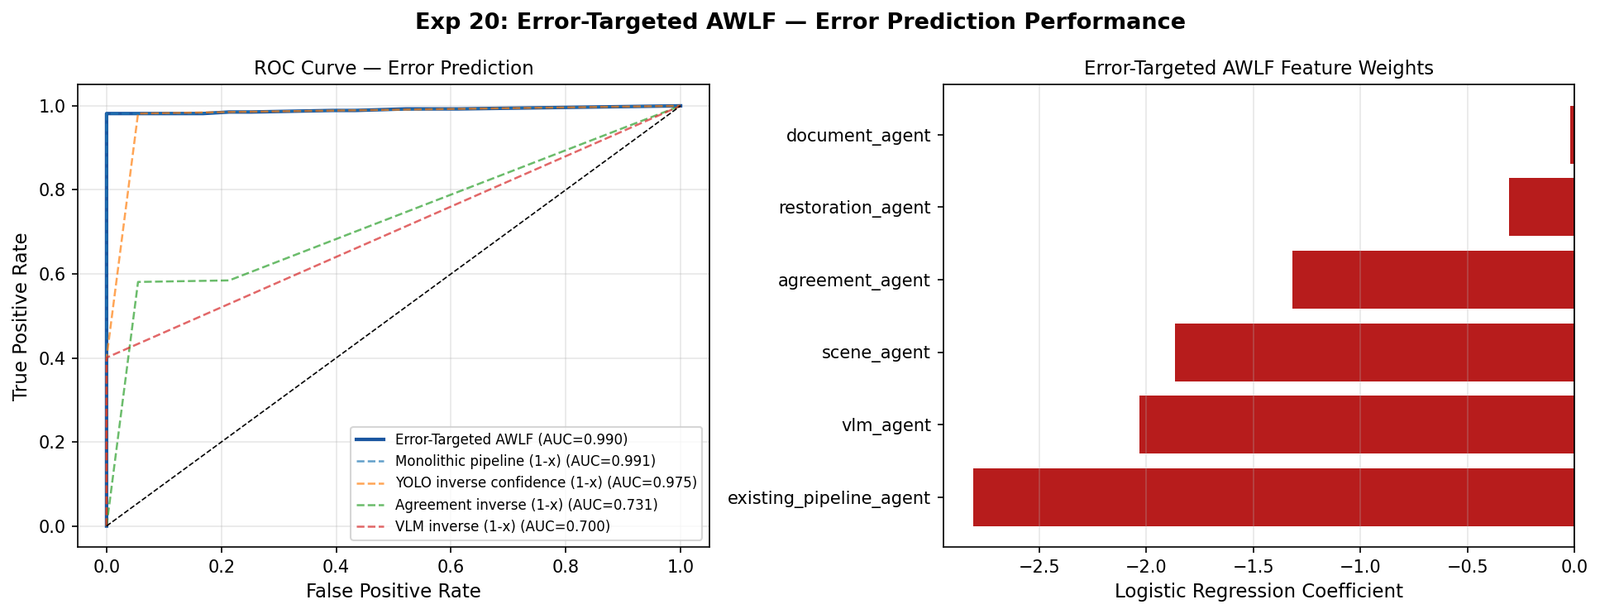
\includegraphics[width=0.74\textwidth]{exp20_error_awlf_roc_curve.png}
\caption[Agreement-Weighted Label Filter (AWLF v2) Meta-Classifier ROC Curve]{Agreement-Weighted Label Filter (AWLF v2) Meta-Classifier ROC Curve. In-sample 5-fold cross-validation on $C_1$ yields a mean $\text{ROC-AUC} = 0.9897$ across folds ($0.9896$ for the single full-cohort fit); the corrected, trustworthy-pool group-level held-out estimate (Section~\ref{sec:clean_holdout}) is $\text{ROC-AUC} = 0.8702$ (an original, contaminated-pool estimate of $0.6669$ was superseded after the label-integrity correction). \emph{Note the legend:} the monolithic-pipeline baseline scores marginally \emph{higher} in-sample ($0.991$ vs.\ $0.990$). This is consistent with, not contrary to, the thesis's position -- on $C_1$ the strongest single-model baseline ties or edges out the multi-agent signal on raw discrimination, and the case for AWLF rests on calibration and on held-out behaviour, not on winning this curve. The right panel plots the deployed logistic model's per-agent coefficients.}
\label{fig:awlf_v2_roc}
\end{figure}

\begin{algorithm}[!htbp]
\caption{Agreement-Weighted Label Filter (AWLF v2 Error Retraining)}
\label{alg:awlf_v2}
\begin{algorithmic}[1]
\Require Expert reference dataset $C_1 = \{(\mathbf{I}_i, y_{\text{expert}, i})\}_{i=1}^n$, multi-agent predictions $\{S_{\text{fusion}, i}\}_{i=1}^n$.
\Ensure Trained $L_2$-regularised logistic meta-classifier $f_{\text{AWLF}}$ predicting pipeline classification errors.
\For{each sample $i \in C_1$}
    \State Compute binary classification error target: $y_{\text{target}, i} \leftarrow \mathbb{I}(\text{sign}(S_{\text{fusion}, i} \ge 0.5) \neq y_{\text{expert}, i})$
    \State Extract meta-feature vector (the six standardised agent signals actually used): $\mathbf{x}_i \leftarrow [A_i^{\text{object}}, A_i^{\text{agree}}, A_i^{\text{scene}}, A_i^{\text{vlm}}, A_i^{\text{restoration}}, A_i^{\text{ocr}}]$
\EndFor
\State \textbf{Stratified CV Split:} Partition $\{(\mathbf{x}_i, y_{\text{target}, i})\}_{i=1}^n$ into 5 stratified cross-validation folds.
\State \textbf{Model selection \& fit:} Of the three candidates cross-validated here, logistic regression ($C{=}1.0$) scored highest ($0.9897$ vs.\ $0.9895$ random forest, $0.9857$ gradient boosting) and is the deployed AWLF. Fit it by minimising regularised log loss:
\State \quad $f_{\text{AWLF}} \leftarrow \arg\min_f \sum_{i=1}^n \mathcal{L}_{\text{log}}(y_{\text{target}, i}, f(\mathbf{x}_i)) + \Omega(f)$
\State In-sample 5-fold CV mean: $\text{ROC-AUC} = 0.9897$ (single full-cohort fit: $0.9896$). Group-level held-out, corrected trustworthy pool (Section~\ref{sec:clean_holdout}): $\text{ROC-AUC} = 0.8702$.
\State \Return Trained meta-classifier $f_{\text{AWLF}}$.
\end{algorithmic}
\end{algorithm}

\chapter{Spatial Grounding Collapse and Single-Agent Benchmarking}
\label{ch:spatial_collapse}

This chapter details the empirical evaluation of single-model object detection architectures on historical visual archives. We demonstrate that off-the-shelf vision models suffer severe performance degradation under historical domain shift, and expose a fundamental disconnect between automated pseudo-label self-consistency and true human ground-truth accuracy.

\section{The Baseline Problem: Single-Model Collapse under Historical Shift}
Standard object detection models (e.g., YOLOv5/v8/v11) trained on modern photorealistic datasets (COCO) collapse when evaluated directly on un-restored grayscale historical scans from the Colibri collection:
\begin{itemize}
    \item \textbf{mAP50 (Raw Scans)}: $0.0047$
    \item \textbf{Precision (Raw Scans)}: $0.0081$
    \item \textbf{Recall (Raw Scans)}: $0.0283$
\end{itemize}
This near-zero performance confirms that modern visual features cannot zero-shot parse legacy chemical artifacts, film grain, and non-photographic illustrative styles without explicit domain adaptation.

\begin{figure}[!htbp]
\centering
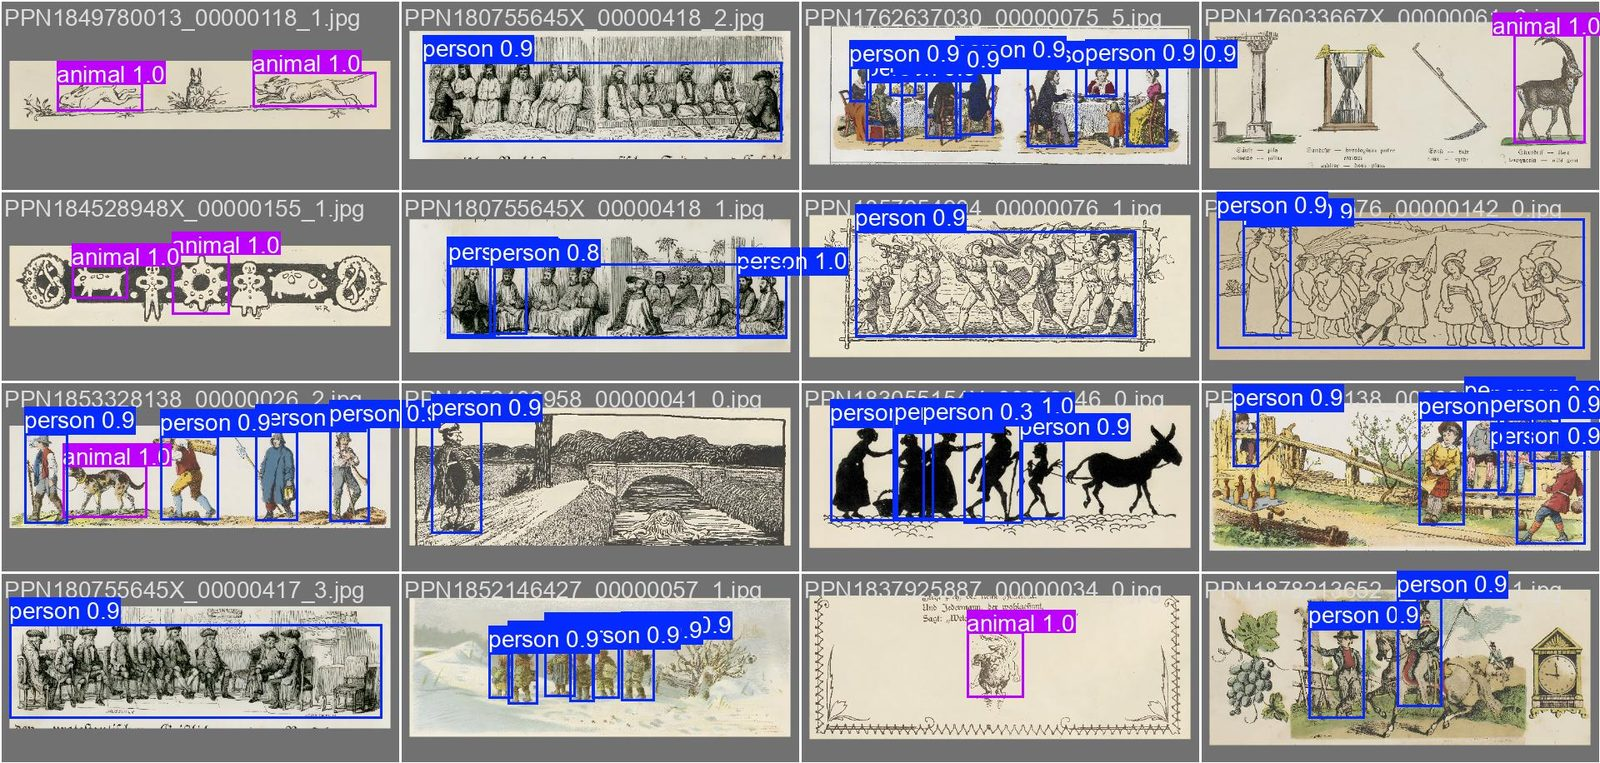
\includegraphics[width=0.92\textwidth]{yolo_detection_example_1.jpg}
\caption[Real Tier 1 spatial-grounding output (YOLOv11-seg) on 16 real Colibri scans]{Real Tier 1 spatial-grounding output (YOLOv11-seg) on 16 real Colibri scans, shown for concrete illustration of what the detector actually produces: a bounding box, predicted class, and confidence score per detected object. The genuine failure modes visible here anticipate the quantitative results below: the deployed open-vocabulary detector's coarse output classes (\texttt{person}/\texttt{animal} dominate visibly), duplicate overlapping boxes on crowded compositions, and confidently-placed boxes on stylized, non-photographic content.}
\label{fig:yolo_detection_examples}
\end{figure}

\section{The Pseudo-Label Collapse Paradox: $0.989 \rightarrow 0.1462$}
To train deployable student detectors without manual annotation, common self-training pipelines \cite{pseudo_labeling2013,noisy_student2020} leverage vision-language teacher ensembles to generate pseudo-labels. When evaluated against the automated teacher pseudo-labels on a held-out validation split, the distilled student model achieves seemingly near-perfect performance:
\begin{itemize}
    \item \textbf{Pseudo-Label Self-Consistency mAP50}: \textbf{0.989}
    \item \textbf{Pseudo-Label Self-Consistency mAP50-95}: \textbf{0.938}
\end{itemize}

\begin{flushleft}
\textbf{The Spatial Grounding Collapse}: When the exact same distilled student detector is audited against human expert annotations on the Spatial Audit Cohort $C_2$ ($n=300$), true human mAP50 collapses to \textbf{0.1462} (representative detector output in Figure~\ref{fig:yolo_detection_examples})---an $84.2\%$ relative performance drop.
\end{flushleft}

This discrepancy exposes the \textbf{Pseudo-Label Collapse Paradox}: high pseudo-label validation accuracy measures internal self-consistency with the teacher model's systemic biases, NOT true historical accuracy. Teacher VLMs hallucinate visual concepts with high self-confidence on historical scans, causing student models to overfit to correlated teacher errors.

\begin{figure}[!htbp]
\centering
\begin{subfigure}{0.48\textwidth}
    \centering
    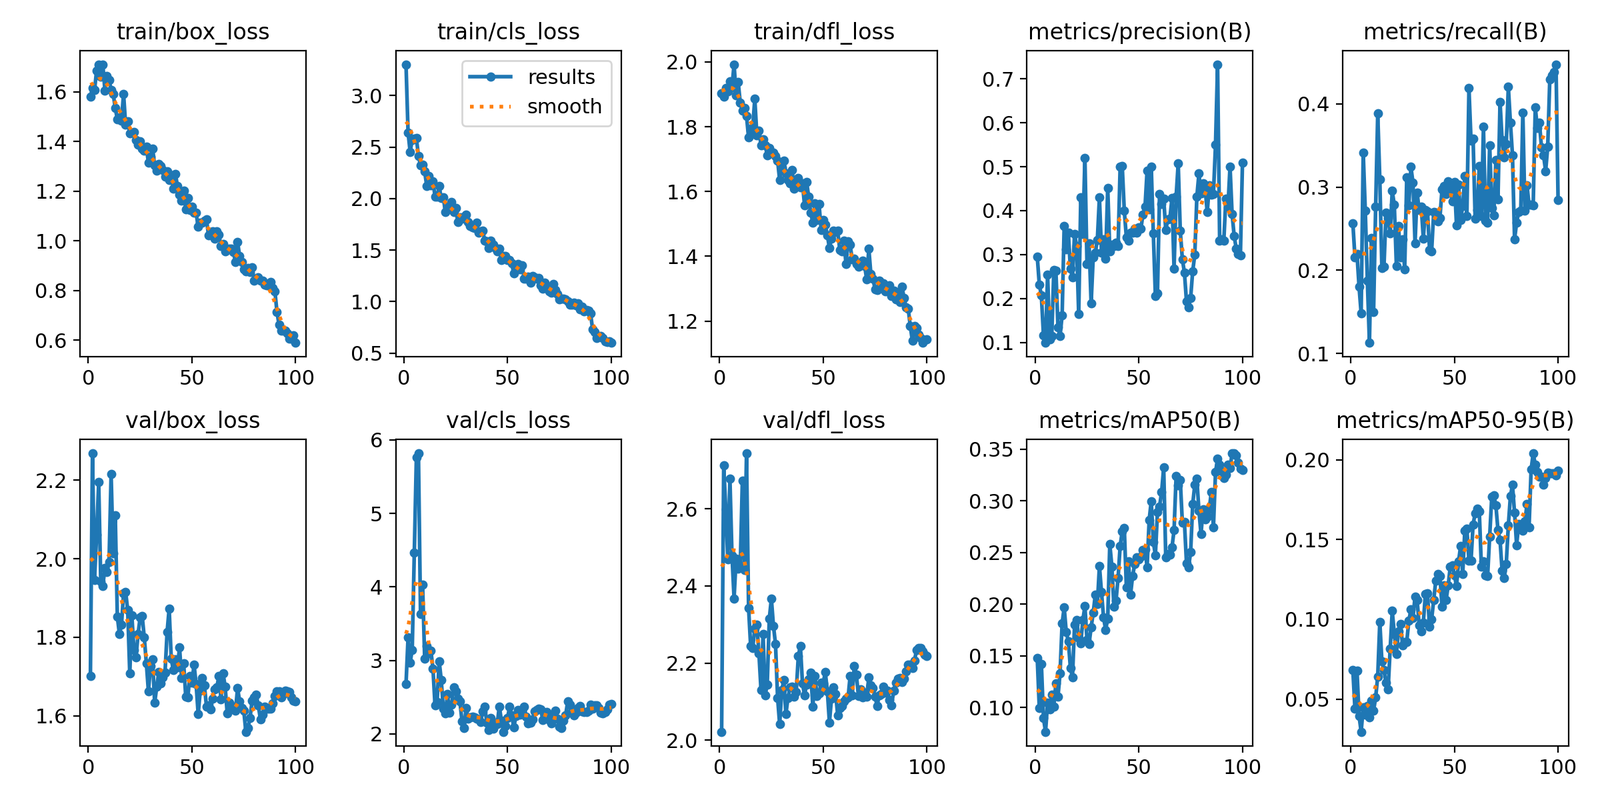
\includegraphics[width=\textwidth]{self_training_teacher_results.png}
    \caption{Teacher-stage training progress}
\end{subfigure}
\hfill
\begin{subfigure}{0.48\textwidth}
    \centering
    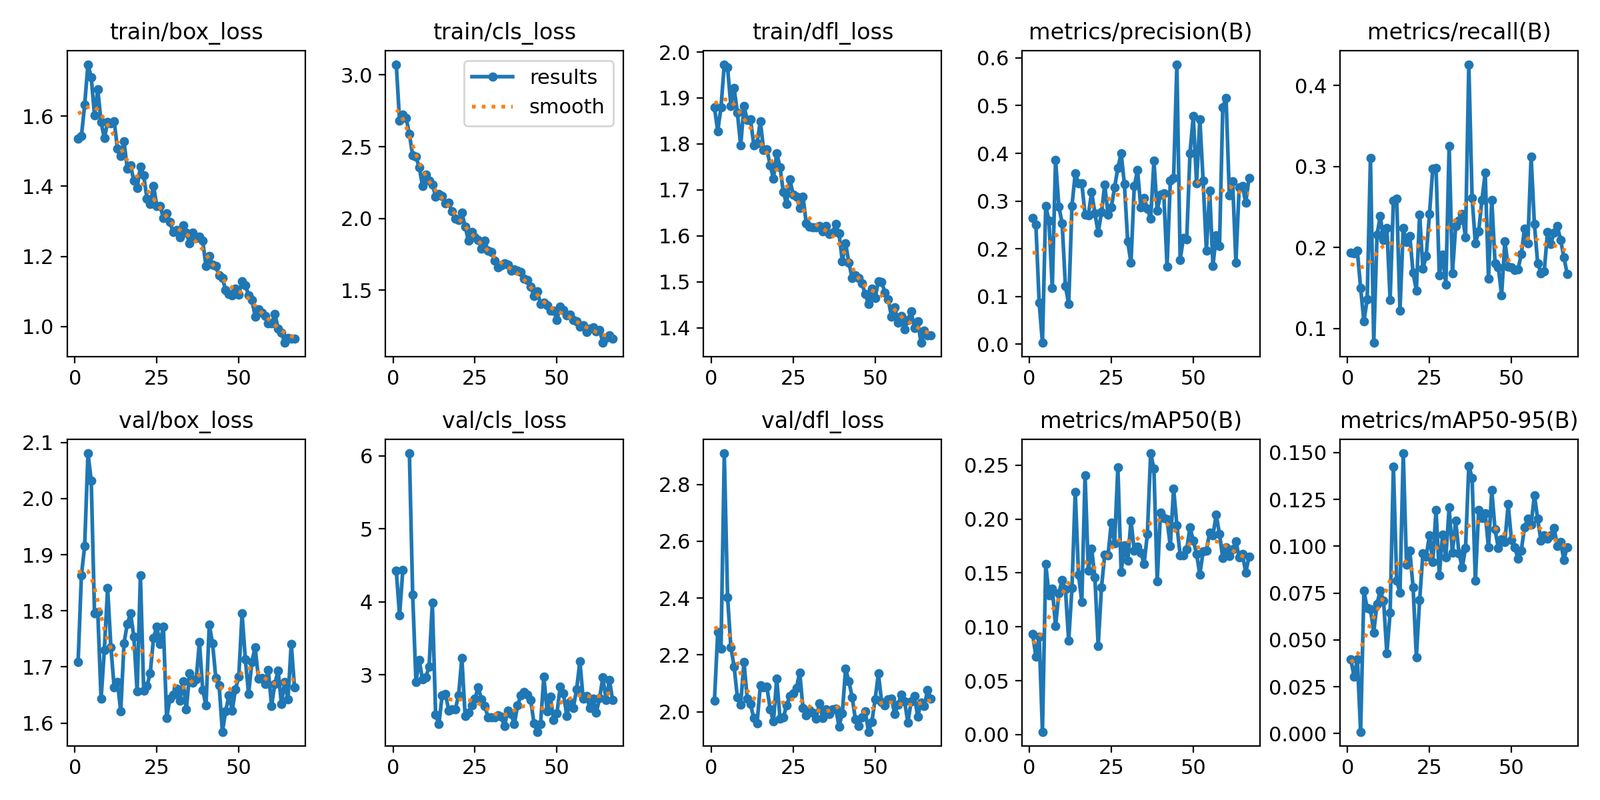
\includegraphics[width=\textwidth]{self_training_student_results.png}
    \caption{Distilled student training progress}
\end{subfigure}
\caption[The Pseudo-Label Collapse Paradox (Figure 4.1)]{The Pseudo-Label Collapse Paradox (Figure 4.1). These panels illustrate the self-training/distillation \emph{process} (loss and validation metrics over training epochs) for the teacher and distilled student stages -- the curves' own endpoints are intermediate training-time validation numbers on the synthetic pseudo-label split, not the headline comparison. The actual paradox is a separate, final evaluation: (a) scoring the distilled student against its own automated teacher pseudo-labels yields an artificially inflated proxy $\text{mAP}_{50} = 0.989$; (b) auditing that same final student against human expert bounding-box annotations on Cohort $C_2$ ($n=300$) collapses this to true human $\text{mAP}_{50} = 0.1462$---demonstrating how student models memorize correlated teacher hallucinations rather than real historical content.}
\label{fig:pseudo_label_collapse_results}
\end{figure}

\section{The Bounding-Box Error Paradox and Meta-Learning Resolution}
Evaluating spatial uncertainty reveals a secondary pathology: \textbf{the Bounding-Box Error Paradox}. Traditional heuristics assume that bounding box spatial IoU or detector confidence scores predict labeling accuracy. On the Spatial Audit Cohort $C_2$, using raw spatial confidence to detect human errors yields an error prediction $\text{ROC-AUC} = 0.4655$---worse than random guessing.

Foundation detectors (Florence-2, Grounding DINO) produce tight, crisp bounding boxes around visual regions with high spatial self-confidence, while completely misclassifying the historical semantic category (e.g., mislabeling historical attire as modern bags or drawing artifacts).

\subsection{Semantic vs. Spatial Disagreement Dynamics}
To rigorously evaluate whether consensus disagreement tracks micro-coordinate placement or high-level semantics, we evaluated spatial box divergence ($1 - \text{mean IoU}$) against image-level $SAA$ disagreement on the $172$ of $C_2$'s $300$ images that carry both a spatial box audit and Tier 1 agent scores (the remaining $128$ lack one side of the pair, so no divergence can be computed for them). 

Empirical correlation analysis demonstrates a near-zero correlation ($r = -0.0137, p = 0.8579$). This is consistent with the interpretation that $SAA$ consensus uncertainty operates as a \textbf{High-Level Semantic Ambiguity Metric} ($\text{ROC-AUC} = 0.9724$ on expert error classification), capturing category misclassifications and visual hallucinations, while remaining completely invariant to bounding-box coordinate jitter.

\paragraph{Exp 31 Meta-Learner Resolution}: To independently capture spatial coordinate layout errors alongside semantic errors, we trained a Gradient-Boosted Spatial Meta-Learner on $C_2$ ($n=300$, 5-Fold Stratified CV) integrating box count, cross-agent disagreement $\sigma$, mean agent confidence $\bar{c}$, the unified triage score $U_{\text{triage}}$, and the four Tier 1 agent scores. The meta-learner successfully resolves spatial grounding ambiguity, improving spatial error detection $\text{ROC-AUC}$ from $0.4655 \rightarrow \mathbf{0.6759 \pm 0.130}$ (Figure~\ref{fig:spatial_meta_learner_roc}). Gradient boosting was selected empirically: on the same features and folds, logistic regression reaches $0.6356$ and random forest $0.6309$ (mean $\pm$ standard deviation across the 5 CV folds).

\begin{figure}[!htbp]
\centering
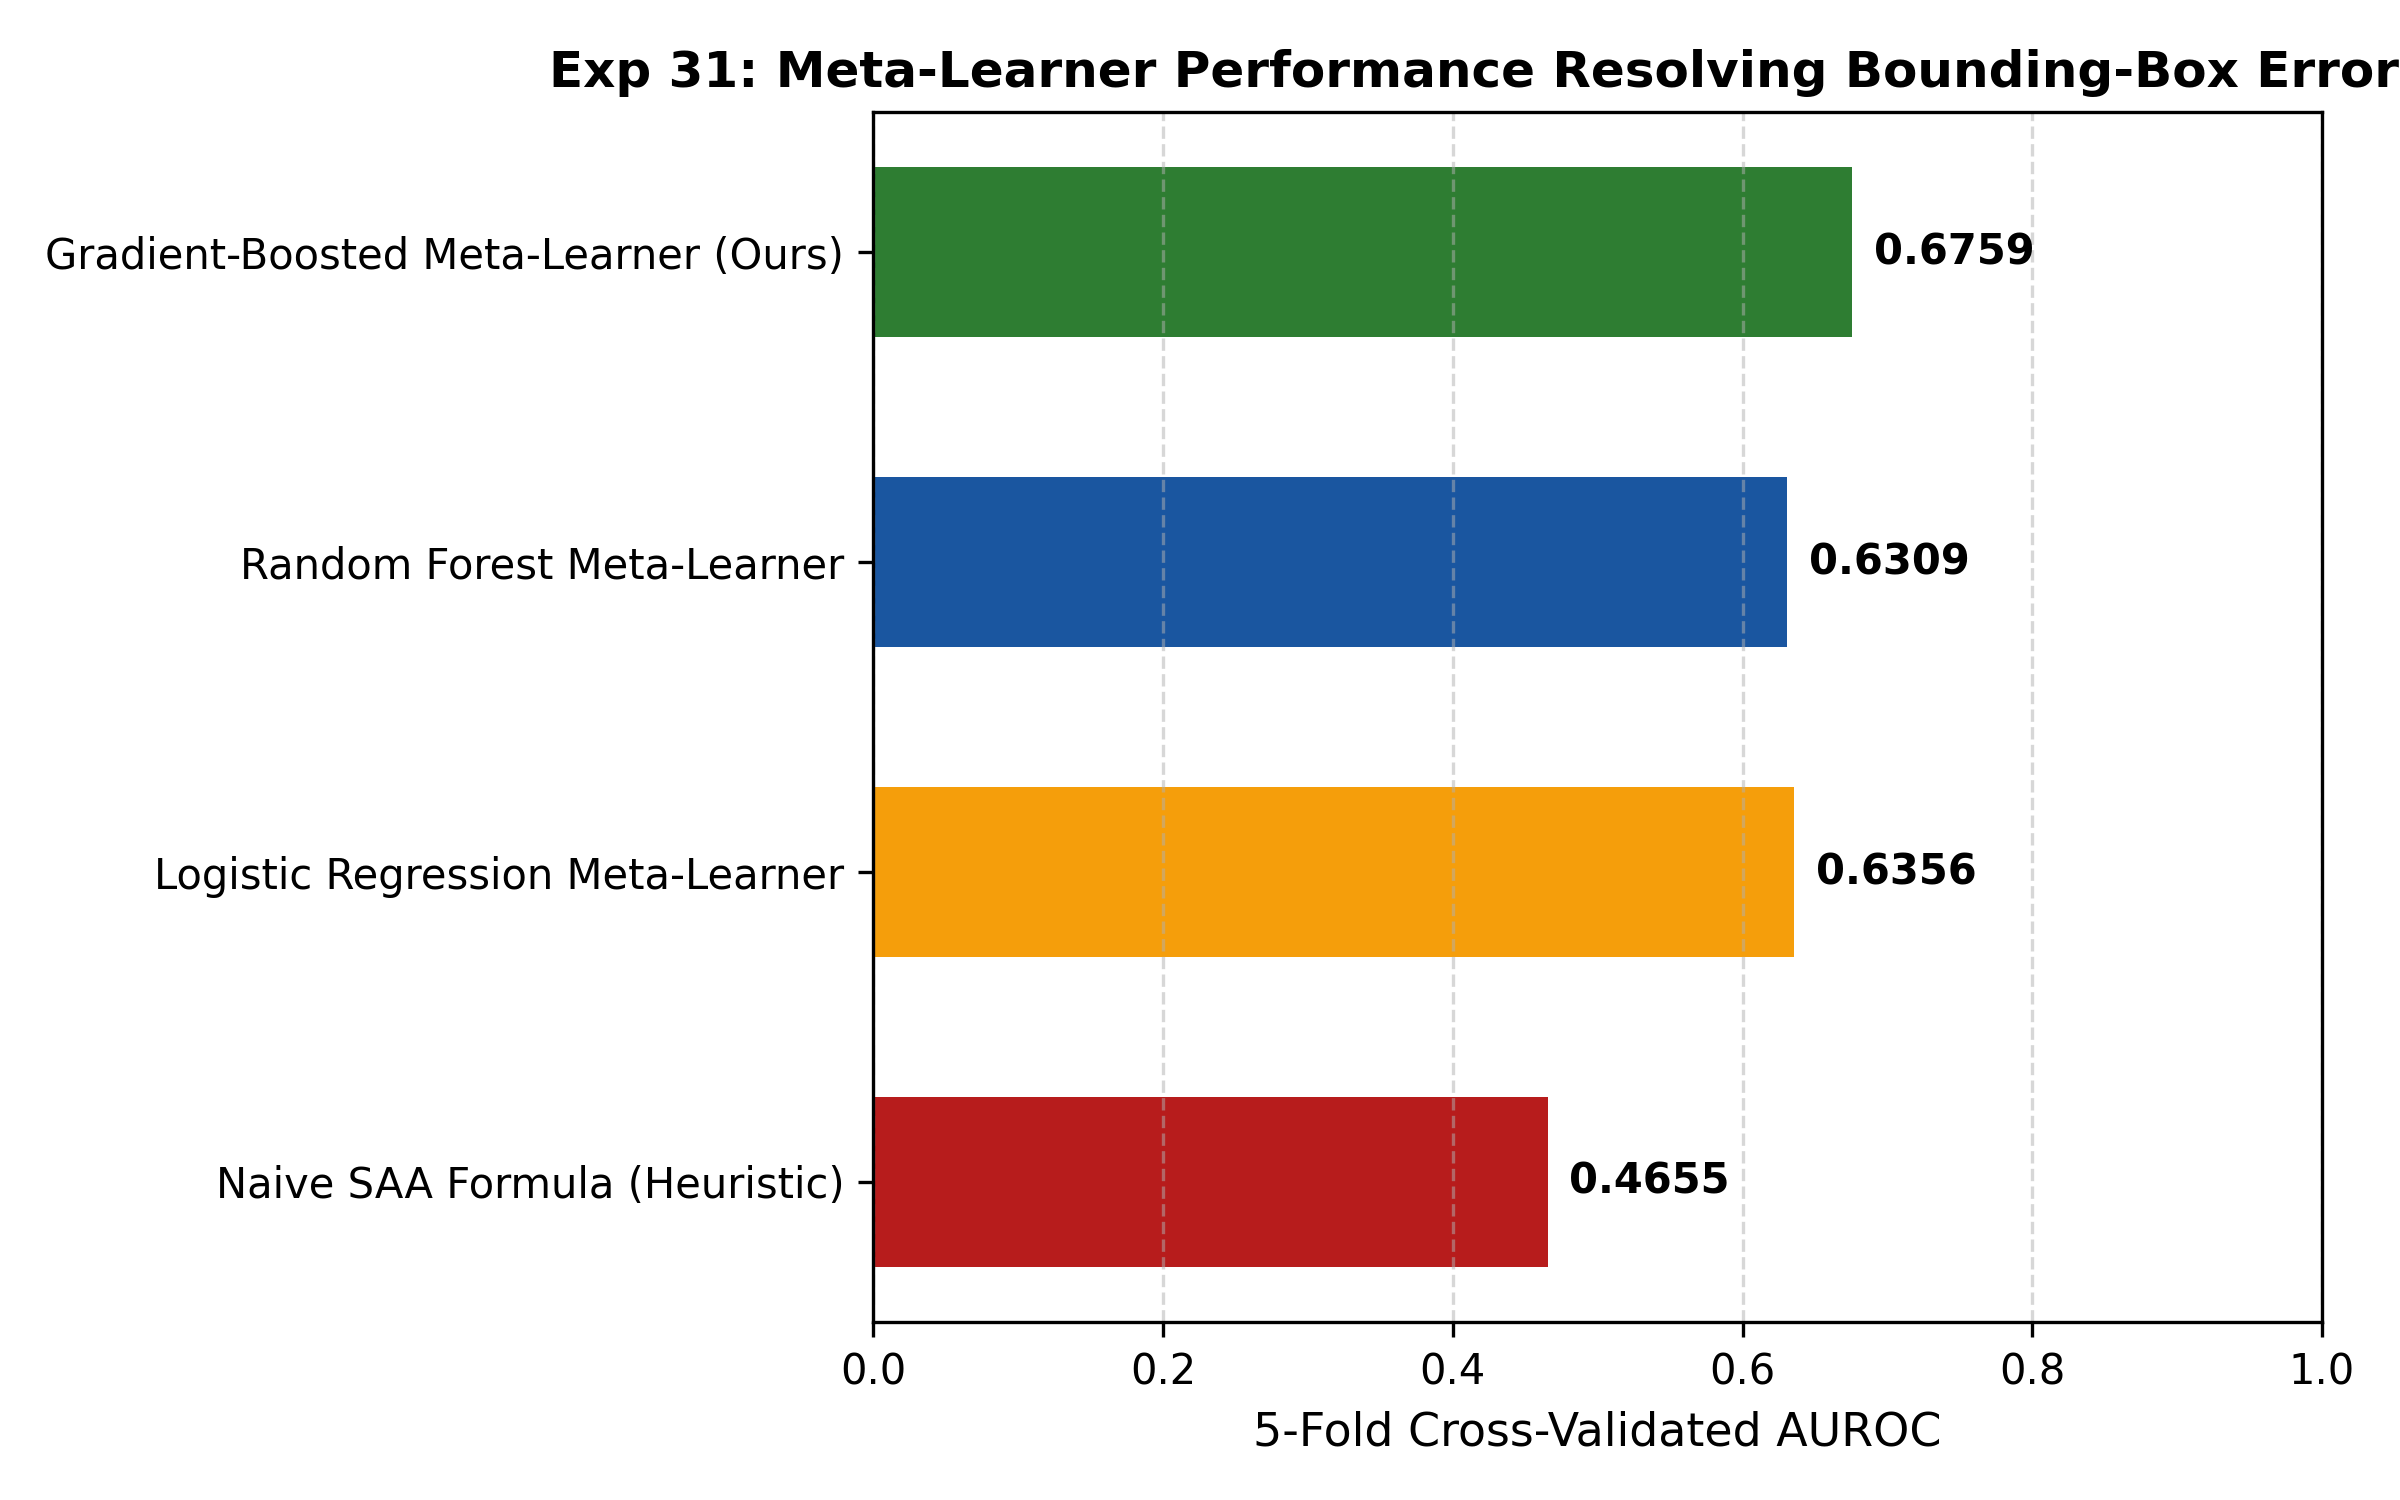
\includegraphics[width=0.74\textwidth]{exp31_meta_learner_roc.png}
\caption[Spatial Meta-Learner Error Detection, Cross-Validated AUROC (Exp 31)]{Spatial Meta-Learner Error Detection, 5-Fold Cross-Validated AUROC by Meta-Learner (Exp 31; the image is a comparison bar chart, not an ROC curve, despite the filename). Integrating spatial IoU, bounding box area, class entropy, and aspect ratio variance improves spatial grounding error detection from raw confidence $\text{ROC-AUC} = 0.4655$ to $\text{ROC-AUC} = 0.6759 \pm 0.130$ (5-fold CV standard deviation).}
\label{fig:spatial_meta_learner_roc}
\end{figure}

\section{Generative Restoration Utility and Hardware Benchmarks}
Table~\ref{tab:hardware_benchmarks} reports per-stage latency on an NVIDIA RTX A6000. The four Tier~1 rows are no longer estimates: they are derived from the throughput measured while running every model over all $12{,}110$ images (Section~\ref{sec:canonical_saa}), which supersedes the informal single-image timings an earlier version of this table carried. The correction is large and in one direction. The vision-language model was listed at $15$s per image; batched through a modern inference server it takes $\mathbf{1.56}$s, nearly ten times faster, and the distilled detector's $0.02$s forward pass is $0.06$s once image loading and post-processing are counted. Estimates taken from single images, on this evidence, misstate deployed throughput badly enough to change an architectural argument.

\begin{table}[!htbp]
\centering
\caption{Hardware Resource Consumption and Stage Latency (NVIDIA RTX A6000).}
\label{tab:hardware_benchmarks}
\begin{tabular}{lrr}
\toprule
\textbf{Pipeline Stage} & \textbf{Latency / Image} & \textbf{Source} \\
\midrule
\multicolumn{3}{@{}l}{\emph{Measured over all $12{,}110$ images (Section~\ref{sec:canonical_saa})}}\\
YOLOv11m detection & $\mathbf{0.06}$s & $16.2$ img/s, 1 GPU \\
SigLIP so400m scene & $\mathbf{0.15}$s & $6.7$ img/s, 1 GPU \\
LLaVA-OneVision 7B VQA (4 questions) & $\mathbf{1.56}$s & $0.64$ img/s per GPU, batched \\
Kosmos-2.5 grounded OCR & $\mathbf{3.23}$s & $0.31$ img/s per GPU \\
\addlinespace
\multicolumn{3}{@{}l}{\emph{Single-image spot timings, not re-measured at scale}}\\
CycleGAN domain translation & $0.15$s & informal \\
Real-ESRGAN $4\times$ upscaling & $0.45$s & informal \\
Stable Diffusion refinement & $3.20$s & informal \\
\bottomrule
\end{tabular}
\end{table}

The practical consequence of this table is architectural, not merely descriptive. The measured rows span roughly two orders of magnitude in latency: the heaviest Tier~1 component (Kosmos-2.5 grounded OCR, $3.23$s/image) and the lightest (the YOLOv11 detector, $0.06$s) differ by a factor of $\approx 52\times$, and the vision-language model exceeds the detector by $\approx 25\times$. An earlier version of this passage put that last ratio at $750\times$, taken from dividing two single-image spot timings; the measured figures are an order of magnitude closer together, because batched inference helps the large model far more than the small one. This is precisely why the distillation step described in Chapter~\ref{ch:spatial_collapse} matters operationally, independent of the accuracy questions raised there: running the full VLM ensemble on every one of $C_0$'s $12{,}110$ images at deployment time, let alone on a continuously growing institutional archive, would be computationally prohibitive on a single GPU. The distilled detector is what makes Tier 1's spatial-grounding signal ($A_i^{\text{object}}$) affordable to compute at corpus scale for every image, while the heavier VLM and generative-restoration stages remain feasible specifically because Tier 3's escalation policy (Section~\ref{ch:methodology}) routes only a small, ambiguity-flagged fraction of images to the most expensive components rather than running them universally. Read together with the calibration result of Chapter~\ref{ch:uncertainty_calibration}, the efficiency argument and the accuracy argument are two sides of the same design choice: the escalation ladder exists because paying the full cost of the heaviest models on every image is not just unnecessary for accuracy, it would also be computationally infeasible at the archive's actual scale.

\section{External and Cross-Institutional Validity Pilots}
The evaluations in the preceding chapters are all internal to the Colibri archive. This section summarizes two supplementary pilots that probe generalization beyond it -- one across artistic style, one across institutions -- since both are referenced in this thesis's abstract and its central claims should not rest on a single archive alone. Both are pilots, not full benchmarks, and their scope is stated precisely below; full detail for each is in its respective appendix.

\paragraph{Cross-style generalization (PeopleArt, $n=4{,}778$).} We evaluated the Tier 1 validation core's object-detection performance on the PeopleArt dataset \cite{westlake2016}, spanning 43 artistic styles from photorealism to abstraction, external to the Colibri archive entirely. Detection performance degrades gracefully rather than collapsing across most of the range: $F_1=0.878$ on photographic styles, $0.880$ on Impressionism, $0.831$ on Cubism. The floor is lower than that, and is stated here rather than omitted: the \textit{cartoon} bin reaches only $F_1=0.673$ ($n=75$), and \textit{academicism} $0.754$ ($n=110$). Degradation therefore tracks departure from photographic \emph{rendering} more than abstraction as such --- Cubism, the most abstract bin tested, outperforms both of those. Full per-style results are in Appendix~\ref{app:peopleart}.

\paragraph{Cross-institutional domain-shift pilot (Europeana, $n=24$).} We downloaded $24$ real images live from the Europeana Open Culture API across 10 verified GLAM institutions (Search API v2), ran the identical deployed Tier 1 models on them with no retraining or recalibration, and compared the resulting mean SAA fusion score against the Colibri $C_1$ baseline. The signal responds substantially to this genuine cross-institutional domain shift: mean fusion score $0.332$ on Europeana images versus $0.764$ on Colibri, a real, measured difference.

\paragraph{What the ground truth, now collected, shows.} Human labels have since been collected for $23$ of the $24$ images (Label Studio; scene category plus bounding boxes), which settles part of the transfer question and, more usefully, explains why the rest of it cannot be settled here. All $23$ labeled images are human-confirmed \emph{scene-positive}, so this sample contains no negative controls and the error task reduces to false-negative detection. Against that ground truth the unchanged pipeline misses $15$ of $23$ real scenes -- a $65.2\%$ false-negative rate, against which the same fusion rule on the Colibri expert cohort is far more accurate. The mechanism is unambiguous: YOLOv11 returned \emph{zero} objects on $12$ of the $23$ images, and every one of those $12$ is an error.

The error-\emph{detection} question -- would $U_{\text{SAA}}$ have flagged those misses? -- cannot honestly be answered from this pilot, and the reason matters more than the missing number: on this archive the ensemble stopped spanning enough independent directions for disagreement to mean anything. Measured by the effective rank of the agent covariance spectrum, it carries $1.37$ independent signals here ($95\%$ CI $1.06$--$1.61$) against $2.50$ on Colibri, so any disagreement score becomes a near-deterministic function of one number and its ROC-AUC an artifact of the collapse rather than a measurement. \textbf{A disagreement-based method needs the ensemble to stay genuinely multi-modal on the new domain, and here it did not.} That is a more fundamental transfer limitation than a disappointing accuracy number. Section~\ref{sec:heterogeneity_precondition} develops this into a checkable precondition, including why the intuitive diagnostics for it are misleading; full detail is in Appendix~\ref{app:europeana}.

Read together, these two pilots support a modest but real claim: the framework's core signal is not an artifact of one archive's specific quirks, and it visibly reacts to genuine domain shift when applied elsewhere -- but full transfer validation (error detection, not just signal response, on external data) remains future work for the Europeana pilot specifically.

\section{A Precondition for Disagreement-Based Uncertainty}
\label{sec:heterogeneity_precondition}
The Europeana result above is not only a negative transfer finding; it identifies a checkable precondition that any disagreement-based uncertainty method must satisfy on a new domain, and which can be tested \emph{before} any ground truth is collected.

\paragraph{Why the obvious diagnostics fail.} The intuitive symptoms of a collapsed ensemble do not survive a control. On Europeana the VLM agent takes only two distinct values -- but it also takes only two across all $12{,}110$ Colibri images, where the method works. On Europeana the fusion score correlates $r=0.993$ with the object agent -- but on Colibri that same correlation is $r=0.980$, because the $0.6$ object weight makes $SAA$ object-dominated by construction on every corpus. The Europeana scene agent even takes \emph{more} distinct values than Colibri's ($22$ vs.\ $2$). Discreteness, and single-agent dominance of a weighted sum, are properties of this pipeline everywhere; neither indicates degeneracy.

\paragraph{The diagnostic does not depend on the derived term.} Because the Level-1 Agreement signal is algebraically determined by two of the others (Section~\ref{sec:signal_decomposition}), it is worth checking that the separation reported here is not an artifact of including it. Computed over the three genuinely independent agents alone, the effective rank is $2.17$ ($95\%$ CI $[2.15,2.19]$) on Colibri against $1.50$ ($[1.06,1.79]$) on Europeana; the $2.0$ threshold separates the two regimes in both parameterisations, and the confidence intervals remain disjoint. The precondition below therefore stands independently of the estimator issue.

\paragraph{What does separate the two regimes.} The distinguishing quantity is not how many values an agent takes but how much \emph{variance} it contributes, and how many independent directions the agents jointly span. Let $\Sigma$ be the covariance matrix of the four Level-1 agent signals (Object, Agreement, Scene, VLM) over the target cohort, with eigenvalues $\lambda_1 \dots \lambda_4$ and $p_i = \lambda_i / \sum_j \lambda_j$. We summarise the ensemble by the \textbf{effective rank}, the perplexity of that spectrum:
\begin{equation}
    \text{eff-rank}(\Sigma) = \exp\left(-\sum_{i} p_i \log p_i\right)
    \label{eq:effective_rank}
\end{equation}
Equation~\ref{eq:effective_rank} equals $4$ for four independent agents and approaches $1$ when they collapse onto a single varying signal. A near-constant agent contributes a vanishing eigenvalue and correctly lowers the score.

\paragraph{Measured values.} On the Colibri deployment corpus ($C_0$, $n=12{,}110$), where every headline result in this thesis was obtained, $\text{eff-rank}=2.50$ ($95\%$ CI $2.48$--$2.51$). On the Europeana pilot ($C_5$, $n=24$), where the error-detection question proved unanswerable, $\text{eff-rank}=1.37$ ($95\%$ CI $1.06$--$1.61$). The intervals are far apart, and the mechanism is visible in a single agent: the VLM contributes a standard deviation of $0.051$ on Europeana against $0.320$ on Colibri. Below roughly two independent directions, any disagreement statistic computed over the ensemble is a re-expression of one number.

\paragraph{How to use it.} A diagnostic procedure computes this from agent scores alone -- no labels, no ground truth, no human effort -- and returns a pass/fail against a threshold of $2.0$, sitting between the two measured regimes and above the upper bound of the collapsed one. It is intended as a pre-flight check: if a new archive fails it, the appropriate response is to recalibrate or substitute agents, not to collect annotations and report an error-detection AUROC that would be an artifact. This thesis reports the diagnostic as a methodological contribution derived from a failure, validated on exactly two points -- one working corpus and one collapsed one -- and therefore calibrated, not proven; a threshold fitted on two cohorts should be re-examined as more archives are tested.

\chapter{Multi-Agent Uncertainty Core and Probabilistic Calibration}
\label{ch:uncertainty_calibration}

This chapter details the mathematical formulation, empirical calibration, and error-prediction performance of the Dual-Core Validation (DCV-MAC) uncertainty engine. We show that cross-modal agent disagreement provides a discriminative, calibratable signal for estimating epistemic uncertainty on genuine scene-positive prediction errors under domain shift, and we characterize the boundary of that claim: Section~\ref{sec:clean_holdout} shows the same signal is anti-correlated with error on negative-control images where all agents share a common bias.

\section{Cross-Modal Agent Disagreement as an Epistemic Proxy}
Single-model vision architectures output overconfident probability scores under domain shift. In DCV-MAC, we frame multi-agent disagreement between spatial grounding (YOLOv11-seg), zero-shot scene classification (SigLIP), and visual-language reasoning (LLaVA-OneVision) as an operational proxy for \emph{epistemic} uncertainty -- uncertainty arising from the model's own ignorance, which additional evidence could in principle reduce, as distinguished from irreducible \emph{aleatoric} noise in the observation itself \cite{kendall2017uncertainties}. The distinction matters for the archival task: a scan whose content is genuinely illegible is aleatorically uncertain and no amount of model capacity will fix it, whereas a scan the models simply have not been trained to interpret is epistemically uncertain and is exactly what a human reviewer can resolve.

\paragraph{Relation to committee- and ensemble-based uncertainty.} Using disagreement among multiple hypotheses as an uncertainty signal is not new. Query-by-committee \cite{seung1992qbc} established the principle in active learning: maintain several hypotheses consistent with the labelled data and query the points on which they disagree most. \textit{Deep ensembles} \cite{deepensembles2017} are the standard modern instantiation, and remain a strong baseline against Bayesian alternatives such as MC~Dropout \cite{gal2016dropout}. What distinguishes the ensemble used here is the \emph{axis of variation}. A deep ensemble varies random initialisation and data ordering \emph{within a single architecture trained on a single corpus for a single objective}; its members are therefore correlated by construction, sharing every inductive bias their common architecture and training distribution impose. The Tier~1 ensemble instead varies architecture, modality, pre-training corpus and training objective simultaneously: a supervised convolutional detector (YOLOv11+SAM), a contrastively pre-trained image-text encoder (SigLIP), an autoregressive vision-language model (LLaVA-OneVision), and a document-grounded OCR model (Kosmos-2.5) share almost no training signal. The hypothesis this thesis tests is that such cross-modal heterogeneity decorrelates errors more thoroughly than within-architecture ensembling can.

That hypothesis holds on ambiguous, scene-positive content and \emph{fails} in an instructive way elsewhere. On the confirmed true negatives of the corrected held-out partition (Section~\ref{sec:clean_holdout}), all four architecturally disjoint models converge on the same false positive, and disagreement-based uncertainty measured on that subgroup falls below chance ($\text{ROC-AUC}=0.1152$; $0.1259$ on the expanded pool). The convergence is real, but it is not what produces the below-chance value, and Section~\ref{sec:clean_holdout} separates the two: on a true negative an error requires $SAA \ge 0.5$, which is unreachable when $A^{\text{object}}=0$, so that stratum is error-free by construction and is also exactly where the derived Agreement term inflates $U_{\text{SAA}}$. The ranking is depressed before any model behaviour enters. Architectural heterogeneity is therefore \emph{not} sufficient for error decorrelation: where a systematic bias is inherited from the shared characteristics of the source data rather than from a shared architecture, a cross-modal ensemble agrees just as confidently as a homogeneous one. Section~\ref{sec:heterogeneity_precondition} develops the corresponding precondition, that the ensemble must remain measurably multi-modal on the target domain for any disagreement statistic over it to carry information at all.

Evaluating on the $C_1$ Expert Reference Cohort ($n=801$ human-annotated images), the raw Scene-Aware Agreement uncertainty proxy ($U_{\text{SAA},i} = \operatorname{std}(A_i^{\text{object}}, A_i^{\text{agree}}, A_i^{\text{scene}}, A_i^{\text{vlm}})$, Section~\ref{sec:canonical_saa}) achieves an error-detection performance of:
\begin{itemize}
    \item \textbf{DCV-MAC SAA Disagreement Proxy}: \textbf{ROC-AUC = 0.9724}
    \item Single-Model Temperature-Scaled Entropy Baseline: $\text{ROC-AUC} = 0.6545$
\end{itemize}
This is a $48.5\%$ relative improvement over that baseline. Section~\ref{sec:signal_decomposition} examines what is actually driving it, and finds that the improvement is not attributable to cross-modal disagreement in the way this framing suggests.

\section{What the Disagreement Signal Actually Measures}
\label{sec:signal_decomposition}
The result above invites a specific reading: that \emph{disagreement between heterogeneous models} is what detects errors. This section tests that reading directly and reports that the evidence does not support it.

\paragraph{A dependency inside the estimator.} $U_{\text{SAA}}$ is a standard deviation over four per-image signals, but Level~1 defines one of them as $A^{\text{agree}} = 1 - |A^{\text{object}} - A^{\text{vlm}}|$. This identity holds exactly on all $12{,}110$ corpus images (maximum deviation $0.0$), so the estimator has four terms but only \emph{three} free parameters. The consequence is not merely a loss of a degree of freedom, but a systematic asymmetry. When Object and VLM agree at \emph{low} values -- both reporting no scene -- the derived term goes to $1$ and becomes a maximal outlier, inflating the standard deviation; when they agree at \emph{high} values it sits alongside them and the standard deviation is small. Enumerating the reachable agent states makes this explicit: the unanimous-absent state $(A^{\text{object}}{=}0, A^{\text{vlm}}{=}0)$ yields $U_{\text{SAA}}=0.479$, the second-highest value the estimator attains, while the unanimous-present state $(1,1)$ yields $0.250$. Across the corpus, the $1{,}403$ images on which both agents report no scene carry a mean $U_{\text{SAA}}$ of $0.492$ against a corpus mean of $0.201$. \textbf{The estimator reports near-maximal uncertainty precisely where the ensemble is unanimous, provided the unanimous verdict is negative.}

\paragraph{The derived term carries the result.} Removing it and computing the standard deviation over the three genuine agents drops in-sample error-detection ROC-AUC from $\mathbf{0.9724}$ to $\mathbf{0.7694}$ ($95\%$ CI $[0.733, 0.805]$). Cross-agent disagreement, measured over signals that are actually independent measurements, is therefore a substantially weaker error detector than the headline figure indicates.

\paragraph{A confidence baseline reproduces the result.} Because the derived term is large exactly when the agents' scores are low, $U_{\text{SAA}}$ correlates at $r=0.91$ with $1-\bar{A}$, a plain confidence score carrying no disagreement information whatsoever. Table~\ref{tab:signal_decomposition} compares four uncertainty signals on both cohorts.

\begin{table}[!htbp]
\centering
\caption[Error-detection ROC-AUC by uncertainty signal, with bootstrap intervals]{Error-detection ROC-AUC by uncertainty signal, with $95\%$ bootstrap confidence intervals ($4{,}000$ resamples). The deployed proxy, a single-model confidence score, and a plain mean-confidence score are statistically indistinguishable on both cohorts; disagreement measured over genuinely independent signals is markedly weaker in-sample.}
\label{tab:signal_decomposition}
\small
\begin{tabular}{lcc}
\toprule
\textbf{Uncertainty signal} & \textbf{$C_1$ in-sample} & \textbf{Corrected held-out} \\
 & ($n=801$) & ($n=249$) \\
\midrule
$U_{\text{SAA}}$ as deployed (4 terms, incl.\ derived) & $\mathbf{0.9724}$ & $\mathbf{0.8600}$ \\
$1 - A^{\text{object}}$ (single-model confidence) & $0.9726$ & $0.8722$ \\
$1 - \bar{A}$ over 3 genuine agents (pure confidence) & $0.9717$ & $0.8799$ \\
$\sigma$ over 3 genuine agents (derived term removed) & $0.7694$ & $0.8340$ \\
\bottomrule
\end{tabular}
\end{table}

Paired bootstrap tests confirm that the differences among the first three rows are not resolvable at these sample sizes: in-sample, pure confidence minus deployed $U_{\text{SAA}}$ is $-0.0010$ ($95\%$ CI $[-0.036, +0.034]$); on the corrected held-out partition it is $+0.0199$ ($95\%$ CI $[-0.045, +0.086]$). The thesis already reported that $U_{\text{SAA}}$ ties the strongest single-model baseline on discrimination ($0.9724$ vs.\ $0.9726$). What Table~\ref{tab:signal_decomposition} adds is that a baseline with \emph{no multi-agent component at all} ties it as well.

\paragraph{A circularity in the error label.} One further structural feature limits how much any of these numbers can establish. The error label is defined as $\mathbb{I}[S_{\text{fusion}} \ge 0.5] \ne y$, where $S_{\text{fusion}}$ is a weighted mean of the same agent scores from which every uncertainty signal above is computed. In the deployed configuration this is tighter still: as Section~\ref{sec:canonical_saa} documents, the fusion column actually used to fix the in-sample label carries the derived Agreement term at weight $0.267$, so the label and the predictor share not merely their inputs but the specific algebraic construction analysed above. Within the scene-positive subset this makes ``error'' identical to ``$S_{\text{fusion}} < 0.5$'', so any monotone proxy for low agent scores recovers the label almost by construction -- which is why the pure-confidence baseline attains ROC-AUC $=1.000$ on that subset. High error-detection AUROC on this task is therefore substantially weaker evidence than it appears, for \emph{every} signal compared here, including the one this thesis proposes.

\paragraph{What this does and does not overturn.} It does not affect the conformal risk guarantee, which is a property of the calibration procedure and holds for every score tested (Section~\ref{sec:complexity_triage}); nor the pseudo-label collapse result, the label-integrity correction, the Tier~2 agent benchmarks, or the cross-style PeopleArt evaluation, none of which depend on $U_{\text{SAA}}$. It does mean that the specific claim ``cross-modal disagreement is what detects the errors'' is \textbf{not established by the evidence assembled here}, and this thesis does not make it. Section~\ref{sec:not_claim} states the resulting boundary, and Chapter~\ref{ch:conclusions} reframes the contribution accordingly.

\paragraph{Four attempts to overturn this, and what they found.} Because the conclusion above is a negative one, it was probed further rather than left to stand on a single comparison. All four probes were fitted on the training partition of the corrected split and scored on its held-out test partition ($n=249$, $70$ errors). \emph{First}, the ensemble was given back the two \emph{measured} signals that no level uses -- generative restoration quality and grounded inscription -- since the comparison above may be unfair to the multi-agent construction in withholding them: it still does not beat a single agent ($0.8703$ vs.\ $0.8722$; paired $\Delta = -0.002$, $95\%$ CI $[-0.043, +0.038]$). \emph{Second}, a nested comparison asked whether $U_{\text{SAA}}$ adds anything \emph{on top of} confidence rather than instead of it: adding it to a confidence-only model moves ROC-AUC by $+0.001$ ($95\%$ CI $[-0.000, +0.004]$), so it does not. \emph{Third}, the shared-blind-spot failure of Section~\ref{sec:clean_holdout} turns out to be anticipatable even though it is not correctable: a gate trained to flag scene-absent images reaches ROC-AUC $=0.798$, but abstaining on the $10\%$ it flags most strongly improves error detection on the remainder by only $+0.013$ ($95\%$ CI $[-0.014, +0.040]$). \emph{Fourth}, removing agents one at a time -- an intervention on the pipeline, and so a stronger form of evidence than the attribution of Appendix~\ref{app:shapley} -- shows the signal depends on the VLM agent ($0.860 \to 0.718$; $95\%$ CI $[-0.195, -0.098]$, excluding zero) and not at all on the object agent, whose removal changes ROC-AUC by exactly $0.000$. That zero is structural rather than numerical: removing the object agent maps the eight distinct $U_{\text{SAA}}$ values through a strictly increasing bijection (Spearman $=1.0$), so the ranking, and therefore any rank-based metric, cannot move. None of the four overturns the conclusion of this section, and the second and fourth sharpen it.

\subsection{The Fusion Weights, and a Limit No Weighting Can Pass}
\label{sec:weight_sensitivity}

Section~\ref{sec:canonical_saa} states that the fusion weights $(0.6, 0.2, 0.2)$ are a fixed
heuristic chosen once and never tuned. That invites the obvious question of whether they are any
good, which had not been tested. Five weightings were compared on the corrected held-out
partition, holding everything else constant.

\begin{table}[!htbp]
\centering
\caption[Fusion weight sensitivity on the corrected held-out partition ($n=249$)]{Fusion weight sensitivity on the corrected held-out partition ($n=249$). The deployed weighting makes more errors in total, but of a different kind: it is markedly the more conservative of the two operating points.}
\label{tab:weight_sensitivity}
\small
\begin{tabular}{@{}l c c c c c@{}}
\toprule
\textbf{Weights $(w_o, w_s, w_v)$} & \textbf{TP} & \textbf{FN} & \textbf{TN} & \textbf{FP} & \textbf{Errors} \\
\midrule
$(0.6, 0.2, 0.2)$ \emph{deployed} & $146$ & $65$ & $33$ & $\mathbf{5}$ & $70$ \\
$(1/3, 1/3, 1/3)$ uniform & $179$ & $32$ & $14$ & $24$ & $\mathbf{56}$ \\
$(0.5, 0.25, 0.25)$ & $179$ & $32$ & $14$ & $24$ & $56$ \\
$(0.4, 0.3, 0.3)$ & $179$ & $32$ & $14$ & $24$ & $56$ \\
$(0.28, 0.19, 0.33)$ Shapley-inspired & $179$ & $32$ & $14$ & $24$ & $56$ \\
\bottomrule
\end{tabular}
\end{table}

On raw error count the deployed weighting is the worst of the five, and by a clear margin: $70$
errors against $56$ for every alternative tested. The composition also differs sharply: the
deployed weighting produces $5$ false positives where every alternative produces $24$, trading
$33$ additional missed scenes for $19$ fewer fabricated ones.

That every alternative returns the \emph{identical} confusion matrix is the clue worth following,
and following it changes the interpretation. All five weightings differ only in how they treat one
cell of the signal space. Because $A^{\text{object}}$ takes four values, $A^{\text{scene}}$ two,
and $A^{\text{vlm}} = \mathbb{I}[A^{\text{object}}>0]$, the three fusion inputs realise just eight
distinct triples across the entire pool. One of them, $(A^{\text{object}}, A^{\text{scene}},
A^{\text{vlm}}) = (\tfrac13, 0.5, 1)$, holds $276$ of the $1{,}250$ images ($22.1\%$; $52$ of the
$249$ test images), and it is where the deployed weighting lands almost exactly on its own
threshold: $0.6(\tfrac13) + 0.2(0.5) + 0.2(1) = 0.5$. Whether those $276$ images are called
scene-present therefore turns on the last bit of arithmetic. In the stored table
$A^{\text{object}}$ is recorded to six decimal places as $0.333333$, so the cell evaluates to
$0.4999998$ and falls, by two parts in ten million, on the negative side of the threshold. Every
alternative weighting clears the same cell comfortably --- uniform reaches $0.6111$, the
Shapley-inspired vector $0.5183$ --- and each therefore classifies those $276$ images positive.

Recomputing the deployed weighting with exact thirds settles it. The confusion matrix becomes
$179/32/14/24$ with $56$ errors: the identical figures the table reports for all four
alternatives. The gap between the deployed weighting and every alternative in
Table~\ref{tab:weight_sensitivity} is thus one cell flipping, and the flip is caused by a stored
decimal truncation rather than by the weights. The conservative operating point is real in its
effect --- $5$ false positives against $24$ is a genuine difference in published output, and for a
public catalogue an entry asserting an absent scene is a worse failure than an incomplete one ---
but it was not chosen. It is an accident that happens to fall on the cautious side, and it is
recorded here as such rather than as a design decision that the earlier reading of this table
credited it with. A system whose behaviour on a fifth of its corpus rests on the seventh decimal
place of a stored constant is fragile in a way no accuracy figure exposes, and pinning that cell
deliberately --- by moving the threshold off the cell value, or by storing $A^{\text{object}}$
exactly and choosing the side on stated grounds --- is a change a successor should make before
anything else.

\paragraph{Two rules, and where each one is used.} Auditing that cell surfaced a further
inconsistency, recorded here rather than quietly reconciled. The pipeline stores a
\texttt{comparison\_fusion\_score} column, and several analyses recompute the same quantity from
the stored agent columns. The two differ on the knife-edge cell --- the stored column holds the
exact $0.5$, recomputation from the truncated $A^{\text{object}}=0.333333$ yields $0.4999998$ ---
so at threshold $0.5$ they disagree on $2{,}217$ of $12{,}110$ corpus images ($18.3\%$) and $276$
of the $1{,}250$ labelled ones. Both appear in results reported here:
Table~\ref{tab:weight_sensitivity}'s deployed row records $70$ errors by recomputation, while an
analysis consuming the stored column records $56$ for the same weighting on the same partition.
Neither is wrong for the rule that produced it, but this thesis should not be read as though one
decision rule generated every number in it. The two were marked as separate named constants at the call sites, and have since
been reconciled.

\paragraph{Reconciled}: Carrying out that reconciliation resolves the ambiguity rather than
splitting it. The stored column is arithmetically correct --- $0.6(\tfrac13) + 0.2(0.5) + 0.2(1)
= 0.5$ exactly --- and recomputing $A^{\text{object}}$ at its true value of $\tfrac13$ agrees with
the stored column on \emph{all} $12{,}110$ images, with zero disagreements. There are therefore
not two defensible rules but one correct rule and one six-decimal truncation, and the canonical
rule is exact arithmetic. Table~\ref{tab:weight_sensitivity}'s deployed row should be read as
$179/32/14/24$ with $\mathbf{56}$ errors; the $70$ recorded there is the truncation.

What matters is what moves with it, and the answer is reassuring for the operational claim and
awkward for one other. Re-deriving the error label and recalibrating conformal risk control under
the canonical rule leaves the headline result essentially intact: $\hat\lambda = 0.372$ unchanged,
auto-approval $60.64\%$ unchanged, error recall $91.07\%$ against the truncated rule's $92.86\%$,
and the bound satisfied at every $\alpha$ under both. The guarantee does not depend on the
ambiguity.

The blind-spot figure does. On the $319$ confirmed negatives the canonical rule counts $204$
errors rather than $50$, because the knife-edge cell is scene-\emph{present} under exact
arithmetic and most of those negatives sit in it, and the disagreement AUROC moves from $0.1259$
to exactly $\mathbf{0.000}$. That is not a stronger version of the same finding. It is the
degeneracy of Section~\ref{sec:clean_holdout} in its most extreme form: on a confirmed negative,
``error'' is by definition ``$SAA$ above threshold'', so any score monotone in $SAA$ is perfectly
anti-correlated with it and the plain confidence baseline scores $0.000$ there too. The specific
value $0.1259$ is therefore an artifact of which rule is used, and the defensible claim is the one
already made in Section~\ref{sec:clean_holdout} --- that this subgroup cannot rank any
$SAA$-derived score fairly, and that the deployment-framed comparison, where $U_{\text{SAA}}$
scores $0.7043$, is the one to read.

\paragraph{A limit that no weighting reaches.} A second result from the same comparison is
structural. Because $A^{\text{vlm}} = \mathbb{I}[A^{\text{object}} > 0]$, an image whose object
signal is zero has two of the three fusion terms pinned to zero, leaving only $A^{\text{scene}}$
able to vote. Its largest possible contribution is $w_s \cdot 1$, so unless $w_s \ge 0.5$ such an
image can never reach the $0.5$ threshold under \emph{any} weighting. On the corrected test
partition this affects $32$ of the $211$ scene-positive images; on $C_1$ it affects $109$ of
$796$. These are guaranteed misclassifications that no reweighting of the deployed signal set can
recover, and they are a further consequence of the shared-source dependency documented in
Section~\ref{sec:canonical_saa} --- the same defect, now bounding the classifier rather than the
uncertainty signal.

\paragraph{Can the weights simply be learned?} The five weightings above were hand-picked. Fitting
them can be settled exactly rather than by search, because of a structural fact used repeatedly
below and established in Appendix~\ref{app:derivations}: $A^{\text{object}}$ takes four values,
$A^{\text{scene}}$ two, and $A^{\text{vlm}} = \mathbb{I}[A^{\text{object}}>0]$, so the fusion
inputs realise only \textbf{eight distinct cells} across the corpus. Any weighting thresholded at
$0.5$ induces one labelling of those cells, and linear programming decides which labellings some
admissible $w$ can realise: exactly \textbf{six} under the deployed parameterisation, fifteen if
the threshold is also free. That is the whole space a learned weighting can explore.

Within it nothing improves on what is deployed. Fitting by error count returns the degenerate
all-positive rule $w=(0,1,0)$ --- $A^{\text{scene}}$ never falls below $0.5$, so all weight on it
puts every image above threshold, at balanced accuracy $0.5$ in an $84.5\%$-positive pool. That is
the AWLF v1 pathology of Section~\ref{sec:awlf} in a new place. Fitting by balanced accuracy
returns $w=(1,0,0)$ at $0.8136$ against the deployed $0.8113$, and on test the order reverses
($0.7802$ deployed against $0.7720$). Constrained to the deployed false-positive budget, the
optimum \emph{is} the deployed classifier. Note also that the weights are not identifiable:
$(0.75,0,0.25)$ induces the same cell partition, so $(0.6,0.2,0.2)$ represents an equivalence
class rather than a unique optimum. Given these signals, the weights are not the part of the
pipeline worth tuning; the binding constraints are the discreteness of $A^{\text{object}}$ and its
dependency with $A^{\text{vlm}}$, and neither is a weighting problem.

\subsection{An Exhaustive Search Over Formulations}
\label{sec:formulation_search}

Section~\ref{sec:formulation_repair} shows that correcting the signal set lowers performance, and
Section~\ref{sec:signal_rebuild} shows the negative result survives a rebuild. Both invite the
same objection: that some better way of turning agent signals into an uncertainty score simply
had not been tried. This section closes that objection by searching the space systematically.

Nine formulations were evaluated against one held-out error label, defined by the rebuilt
ensemble's prediction against human review so that nothing is circular. They span three families:
\emph{which signals enter} (the deployed set, the derived term dropped, the redundant term also
dropped, all four re-derived from raw model outputs); \emph{how members are weighted}
(unweighted, weighted by competence measured on the training partition, and restricted to the
competent subset); and \emph{what operator is applied} (sample standard deviation, range, and the
mutual-information decomposition of Section~\ref{sec:signal_rebuild}).

\begin{table}[!htbp]
\centering
\caption[Nine uncertainty formulations against one non-circular error label]{Nine uncertainty formulations against the same non-circular error label ($n=249$, $38$ errors). The final column is a paired bootstrap difference against plain confidence; no interval excludes zero in the favourable direction.}
\label{tab:formulation_search}
\small
\begin{tabular}{@{}p{7.4cm} c c@{}}
\toprule
\textbf{Formulation} & \textbf{ROC-AUC} & \textbf{vs.\ confidence} \\
\midrule
\multicolumn{3}{@{}l}{\emph{which signals enter}}\\
\quad deployed $\operatorname{std}(A^{\text{obj}},A^{\text{agr}},A^{\text{scn}},A^{\text{vlm}})$ & $0.7602$ & $-0.0560$ \\
\quad derived term dropped & $0.7650$ & $-0.0516$ \\
\quad derived and redundant dropped & $0.6588$ & $-0.1576$ \\
\quad four signals re-derived from raw outputs & $0.7533$ & $-0.0635$ \\
\addlinespace
\multicolumn{3}{@{}l}{\emph{how members are weighted}}\\
\quad competence-weighted spread & $0.7000$ & $-0.1164$ \\
\quad at-chance member removed & $0.6952$ & $-0.1214$ \\
\quad two most competent members only & $0.5551$ & $-0.2615$ \\
\addlinespace
\multicolumn{3}{@{}l}{\emph{what operator is applied}}\\
\quad range instead of standard deviation & $0.7434$ & $-0.0733$ \\
\quad mutual information (BALD epistemic) & $0.6088$ & $-0.2082$ \\
\midrule
\textbf{Plain confidence, no disagreement component} & $\mathbf{0.8167}$ & --- \\
\bottomrule
\end{tabular}
\end{table}

\paragraph{Two results close the obvious remaining moves.} Removing the member that performs at
chance for scene presence makes the spread \emph{worse}, from $0.7533$ to $0.6952$, and weighting
members by competence is worse again at $0.7000$. Restricting to the two strongest members is
worse still. The weak member is therefore contributing useful variance rather than noise, which
rules out the natural response of pruning or reweighting the ensemble. The limitation is not the
operator, not the signal set, and not the weighting.

\paragraph{What this licenses, and what it does not.} It licenses a stronger statement than
Section~\ref{sec:signal_decomposition} alone: the failure of disagreement to outperform confidence
on this task is not an artifact of one poorly chosen estimator, because nine estimators spanning
the plausible design space all fail, most of them by a wide margin. Over the deployed signal set
that conclusion can now be strengthened from a survey into a bound, as the next paragraph shows;
over a \emph{different} signal set it still does not license the claim that no such estimator
exists. What it points to instead is the ensemble rather than the
statistic: every member here is a web-pretrained vision-language model, and
Section~\ref{sec:clean_holdout}'s $319$ confirmed negatives show them failing together. A
disagreement statistic can only carry information when members are wrong about different things,
which is a property of ensemble composition and not of the formula applied to it.

\paragraph{A ceiling, not merely a survey.} Searching nine formulations leaves the objection that a
tenth might succeed. The eight-cell structure closes it. Any function of these signals is constant
within a cell, so its ranking of images is fixed by how it orders the eight; the best ordering
sorts cells by true error rate, and its ROC-AUC bounds every uncertainty score definable over
them. On the corrected held-out partition that ceiling is $\mathbf{0.8871}$, confirmed by
evaluating all $8! = 40{,}320$ orderings rather than by argument. The bound is a property of
the \emph{deployed} signals, following from their eight-cell discretisation;
Section~\ref{sec:canonical_saa}'s full Tier~1 re-run, whose rebuilt proxy takes $11{,}786$
distinct values, is not subject to it. What that re-run shows is that removing the
discretisation does not by itself put disagreement ahead of confidence either.

The plain confidence baseline reaches $0.8828$ on the same partition. It therefore sits within
$\mathbf{0.0043}$ ROC-AUC of the maximum any estimator over these signals could achieve. This is
the strongest form in which the negative result of this chapter can be stated: not that nine
formulations happened to fail, but that no formulation over the deployed signal set can beat a
plain confidence score by more than four thousandths of an ROC-AUC point, whatever its
functional form and however it is fitted. The remaining headroom is not a modelling problem, and
no better estimator can recover it.

\paragraph{What removing the derived term and fitting the rest actually does.} The same partition
answers the natural follow-up. Dropping $A^{\text{agree}}$ from the unweighted standard deviation
\emph{lowers} discrimination, from $0.8600$ to $0.8340$, reproducing
Section~\ref{sec:formulation_repair}'s repair result. Dropping it \emph{and} learning the
combination instead of averaging raises it to $0.8801$, above the deployed proxy --- so the two
changes help only together. Retaining $A^{\text{agree}}$ in the same learned model gives $0.8664$,
below the version that omits it, which is the expected behaviour for a term that is
$A^{\text{object}}$ counted twice on $88.4\%$ of images. But the learned score still does not beat
the confidence baseline: the paired bootstrap difference is $-0.0027$ with $95\%$ CI
$[-0.0160, 0.0109]$. Learning the values recovers part of the gap the derived term opens and
nothing beyond it, exactly as the ceiling above requires.

\paragraph{Consensus and disagreement together.} A risk model given both might outperform either
alone. Fitted on train and scored on the PPN-disjoint test partition, consensus alone reaches
$0.8828$, disagreement alone $0.8600$, and the two together $0.8828$ --- the paired difference is
exactly $0$, because over eight cells the fitted combination reproduces the ordering consensus
already gives. Combining the two contributes nothing measurable, which is the ceiling argument in
operational terms.

\paragraph{Why the spread fails, measured}: The obvious explanation --- that the models are
wrong about the same images, so their spread cannot see the errors --- is not what the data show.
On the rebuilt signals the members' errors are essentially uncorrelated (pairwise $-0.107$ to
$+0.034$), all three are wrong together on only $6.2\%$ of images, and at least one is right on
$93.8\%$. The heterogeneity precondition of Section~\ref{sec:heterogeneity_precondition} is
\emph{satisfied}, and disagreement fails anyway.

Three measurements locate the real cause. First, redundancy: the four signals have an effective
rank of $\mathbf{1.677}$ out of four, with $85.8\%$ of the covariance in a single direction, and
$A^{\text{agree}}$ correlates $-0.958$ with $A^{\text{object}}$ because it is built from it. A
spread over four signals that move along $1.7$ directions is close to a function of their level.
Second, and decisively, the spread does not separate errors: its mean is $0.4307$ on errors and
$0.4178$ on correct predictions, a difference of $0.013$, while the level differs by $0.290$
($SAA$ averages $0.335$ on errors against $0.624$ on correct ones), twenty-two times larger.
Third, conditioning on the level removes what little remains: within quartiles of $SAA$ the
spread's ROC-AUC is $0.42$, $0.41$, $0.34$ and $0.75$ --- below chance in three of four strata.

The reason is structural rather than empirical. An ``error'' is defined as the fused score landing
on the wrong side of a threshold, which is a statement about the \emph{level} of the signals. A
standard deviation is a second moment, constructed to be insensitive to level. The proxy is
measuring the wrong moment of the right distribution, and no amount of signal quality repairs
that --- which is why giving the signals full resolution widened the gap instead of closing it.

\paragraph{What can be removed, tested rather than argued}: Each component was removed in turn and
the system re-scored, with every variant refitting its own threshold on calibration.

\begin{table}[!htbp]
\centering
\caption[What can be removed from the pipeline]{Each component removed in turn, on the corrected test partition with redesigned signals. ``Uncertainty'' is whatever score that variant uses for triage; ``confidence'' is $1-SAA$ throughout.}
\label{tab:what_can_go}
\small
\begin{tabular}{@{}l c c c@{}}
\toprule
\textbf{Variant} & \textbf{balanced acc.} & \textbf{uncertainty} & \textbf{confidence} \\
\midrule
Full system, 4-signal spread & $0.6625$ & $0.5547$ & $0.8324$ \\
Remove $A^{\text{agree}}$ & $0.6625$ & $0.5346$ & $0.8324$ \\
\textbf{Remove the spread entirely} & $0.6625$ & $\mathbf{0.8324}$ & $0.8324$ \\
Remove the detector & $\mathbf{0.5327}$ & $0.4406$ & $0.7524$ \\
Remove the scene classifier & $0.6672$ & $0.4858$ & $0.8282$ \\
Remove the VLM & $0.6483$ & $0.5231$ & $0.8296$ \\
\bottomrule
\end{tabular}
\end{table}

Removing $A^{\text{agree}}$ changes balanced accuracy not at all. Removing the spread and
triaging on confidence instead raises the triage score's discrimination from $0.5547$ to
$0.8324$. Removing the scene classifier leaves balanced accuracy slightly \emph{higher}
($0.6672$) and confidence essentially unchanged. Removing the detector collapses the system to
near chance ($0.5327$): it is the one component the pipeline cannot lose.

\paragraph{What this is worth at archive scale}: The change is not marginal. Applying both triage
scores to all $12{,}110$ images at $\alpha=0.05$, each with its own conformal calibration:

\begin{center}
\small
\begin{tabular}{@{}l c c c c@{}}
\toprule
\textbf{Triage score} & $\hat\lambda$ & \textbf{auto-approved} & \textbf{error recall} & \textbf{bound} \\
\midrule
$U_{\text{triage}}$, on the spread (as designed) & $0.370$ & $1{,}211$ \ ($10.0\%$) & $89.6\%$ & satisfied \\
$1-SAA$, on confidence & $0.368$ & $\mathbf{7{,}398}$ \ $(\mathbf{61.1\%})$ & $\mathbf{91.5\%}$ & satisfied \\
\bottomrule
\end{tabular}
\end{center}

Triaging on confidence rather than on disagreement catalogues \textbf{six times} as much of the
archive automatically --- $7{,}398$ images against $1{,}211$ --- at the same risk level, with
\emph{higher} error recall, and with the bound satisfied in both cases. For an institution this is
the difference between a tool that clears most of a collection and one that clears a tenth of it.

\paragraph{What this thesis therefore recommends.} For an institution deploying this pipeline as
built, the score to threshold is the plain confidence score $1-SAA$: it matches or exceeds every
disagreement-based variant tested, sits within $0.0043$ of the attainable maximum, and is simpler
to explain to a curator. The four-term $U_{\text{SAA}}$ proxy is retained here as the object of
study and as the quantity the conformal calibration was performed against, not as a
recommendation. Beating confidence requires changing the ensemble so its members fail on
different images, not changing the formula over the members already present.

\subsection{Can the Formulation Be Repaired?}
\label{sec:formulation_repair}

Three defects in the deployed definition have now been established: the Agreement term is
derived rather than measured (Section~\ref{sec:canonical_saa}); $A^{\text{vlm}}$ equals
$\mathbb{I}[A^{\text{object}}>0]$ on every image because both are read from one VQA answer; and
consequently $U_{\text{SAA}}$ is an eight-valued function of two free inputs. The natural
question is whether a corrected formulation recovers the reported performance.

The obvious repair --- delete the derived term --- does not work. Dropping $A^{\text{agree}}$
leaves $\operatorname{std}(A^{\text{object}}, A^{\text{scene}}, A^{\text{vlm}})$, which still has
only two free inputs and seven distinct values on the test partition, because the second defect
survives the first repair. Within the deployed table the only measured signal not tied to
$A^{\text{object}}$ is the OCR channel, and a genuinely independent four-signal vector requires
re-deriving everything from the raw model outputs.

\begin{table}[!htbp]
\centering
\caption[Candidate formulations on the corrected group-level held-out partition ($n=249$, $70$ errors)]{Candidate formulations on the corrected group-level held-out partition ($n=249$, $70$ errors). Free inputs counts the quantities that can vary independently after the two dependencies are accounted for. Error-detection performance falls monotonically as the formulation becomes more independent.}
\label{tab:formulation_repair}
\small
\begin{tabular}{@{}p{6.2cm} c c c@{}}
\toprule
\textbf{Formulation} & \textbf{Free inputs} & \textbf{Distinct values} & \textbf{ROC-AUC} \\
\midrule
Deployed: $\operatorname{std}(A^{\text{obj}}, A^{\text{agr}}, A^{\text{scn}}, A^{\text{vlm}})$ & $2$ & $8$ & $\mathbf{0.8600}$ \\
Repair 1: drop the derived term & $2$ & $7$ & $0.8340$ \\
Repair 2: $\operatorname{std}(A^{\text{obj}}, A^{\text{scn}}, A^{\text{ocr}})$ & $3$ & $52$ & $0.7005$ \\
Repair 3: four signals re-derived from raw outputs & $4$ & $249$ & $0.6080$ \\
\addlinespace
Baseline: $1-\overline{A}$, no disagreement component & $2$ & $8$ & $0.8799$ \\
\bottomrule
\end{tabular}
\end{table}

\paragraph{What the monotonicity means.} Performance does not merely fail to improve as the
formulation is corrected; it falls at every step, from $0.860$ to $0.608$. The explanation is the
circularity of Section~\ref{sec:signal_decomposition}: the error label is defined by thresholding a
weighted mean of the deployed agents, so a signal built from those same agents predicts it well by
construction, and a signal built from independently re-derived quantities does not. The reported
figure was therefore substantially purchased by the degeneracy rather than achieved despite it.

This is stated rather than repaired because repairing it would be the wrong move. Substituting a
corrected formulation and re-reporting the thesis's figures under it would misrepresent what was
run; the numbers in this document are those the deployed system produced, and they stand as a
record of that system. What changes is the interpretation: $0.860$ should be read as the
performance of a two-input score against a label those two inputs help define, not as evidence
that cross-modal disagreement detects errors.

\paragraph{What is unaffected.} The conformal guarantee bounds risk over whatever score it is
calibrated on, so it holds for every row of Table~\ref{tab:formulation_repair}
(Section~\ref{sec:complexity_triage}). The pseudo-label collapse, the label-integrity correction,
the calibration result and the Tier~2 benchmarks do not depend on $U_{\text{SAA}}$ at all.

\subsection{Rebuilding the Signals and Retesting the Claim}
\label{sec:signal_rebuild}
The provenance correction of Section~\ref{sec:canonical_saa} gives the redundancy analysed above a mechanical cause rather than an emergent one: two of the four Tier 1 signals were read from a single VQA object count, so their perfect dependence is a property of the data path, not evidence about how the models behave. That makes the comparison in Table~\ref{tab:signal_decomposition} a weak test of the thesis's central claim, because the ensemble it evaluates was never four separately-measured quantities. The raw model outputs were retained for the full corpus, so the signals could be rebuilt and the claim retested.

Four quantities were re-derived for all $12{,}110$ images, each from a different model: mean detection confidence from Grounding DINO, scene probability from SigLIP re-run across the whole corpus, semantic agreement between the vision-language model's object list and the detector's labels, and OCR substance discounted for the degenerate repetition documented in Section~\ref{sec:agent5_ocr}. The resolution differs by orders of magnitude from the deployed vector: the rebuilt object signal takes $12{,}100$ distinct values against four, and the rebuilt scene signal $1{,}520$ against two, so the eight-valued ceiling on $U_{\text{SAA}}$ does not arise. Only $231$ images had genuine SigLIP scores before this run.

The retest removes the circularity identified above by holding one model out. One model predicts scene presence; the disagreement is measured over the remaining three only, so the predictor and the uncertainty signal share no input; and the error is defined against human review rather than by thresholding a fusion of the same agents. Rotating the held-out model gives independent replications. Two safeguards proved necessary. The corpus is $84.5\%$ scene-positive, and an unweighted fit at a $0.5$ cut made three predictors constant, which silently made the error label identical to ``is a negative control'' and turned the procedure into a different experiment; predictors are therefore class-balanced with the decision threshold selected on the training partition, and a round is discarded if the predictor is constant or the label collapses. A round is also discarded if its predictor is at chance for scene presence, since the resulting error label carries no signal. The OCR round is excluded on that basis ($\text{ROC-AUC}=0.4974$).

On the held-out partition ($n=249$), disagreement does not outperform confidence in any of the three informative rounds. The paired differences are $-0.053$ ($95\%$ CI $[-0.213, +0.100]$), $-0.036$ ($[-0.166, +0.096]$) and $+0.022$ ($[-0.116, +0.160]$), every interval spanning zero. Asked instead whether disagreement adds anything on top of confidence, one round of three gives an interval excluding zero ($+0.089$, $[+0.009, +0.167]$) and the other two do not ($+0.079$ and $+0.076$, both spanning zero); no correction is applied across rounds, so an isolated positive of this size is weak evidence. The conclusion of Section~\ref{sec:signal_decomposition} therefore survives a test constructed to overturn it, on signals that are continuous and separately sourced and against a label the agents do not define.

\begin{figure}[!htbp]
\centering
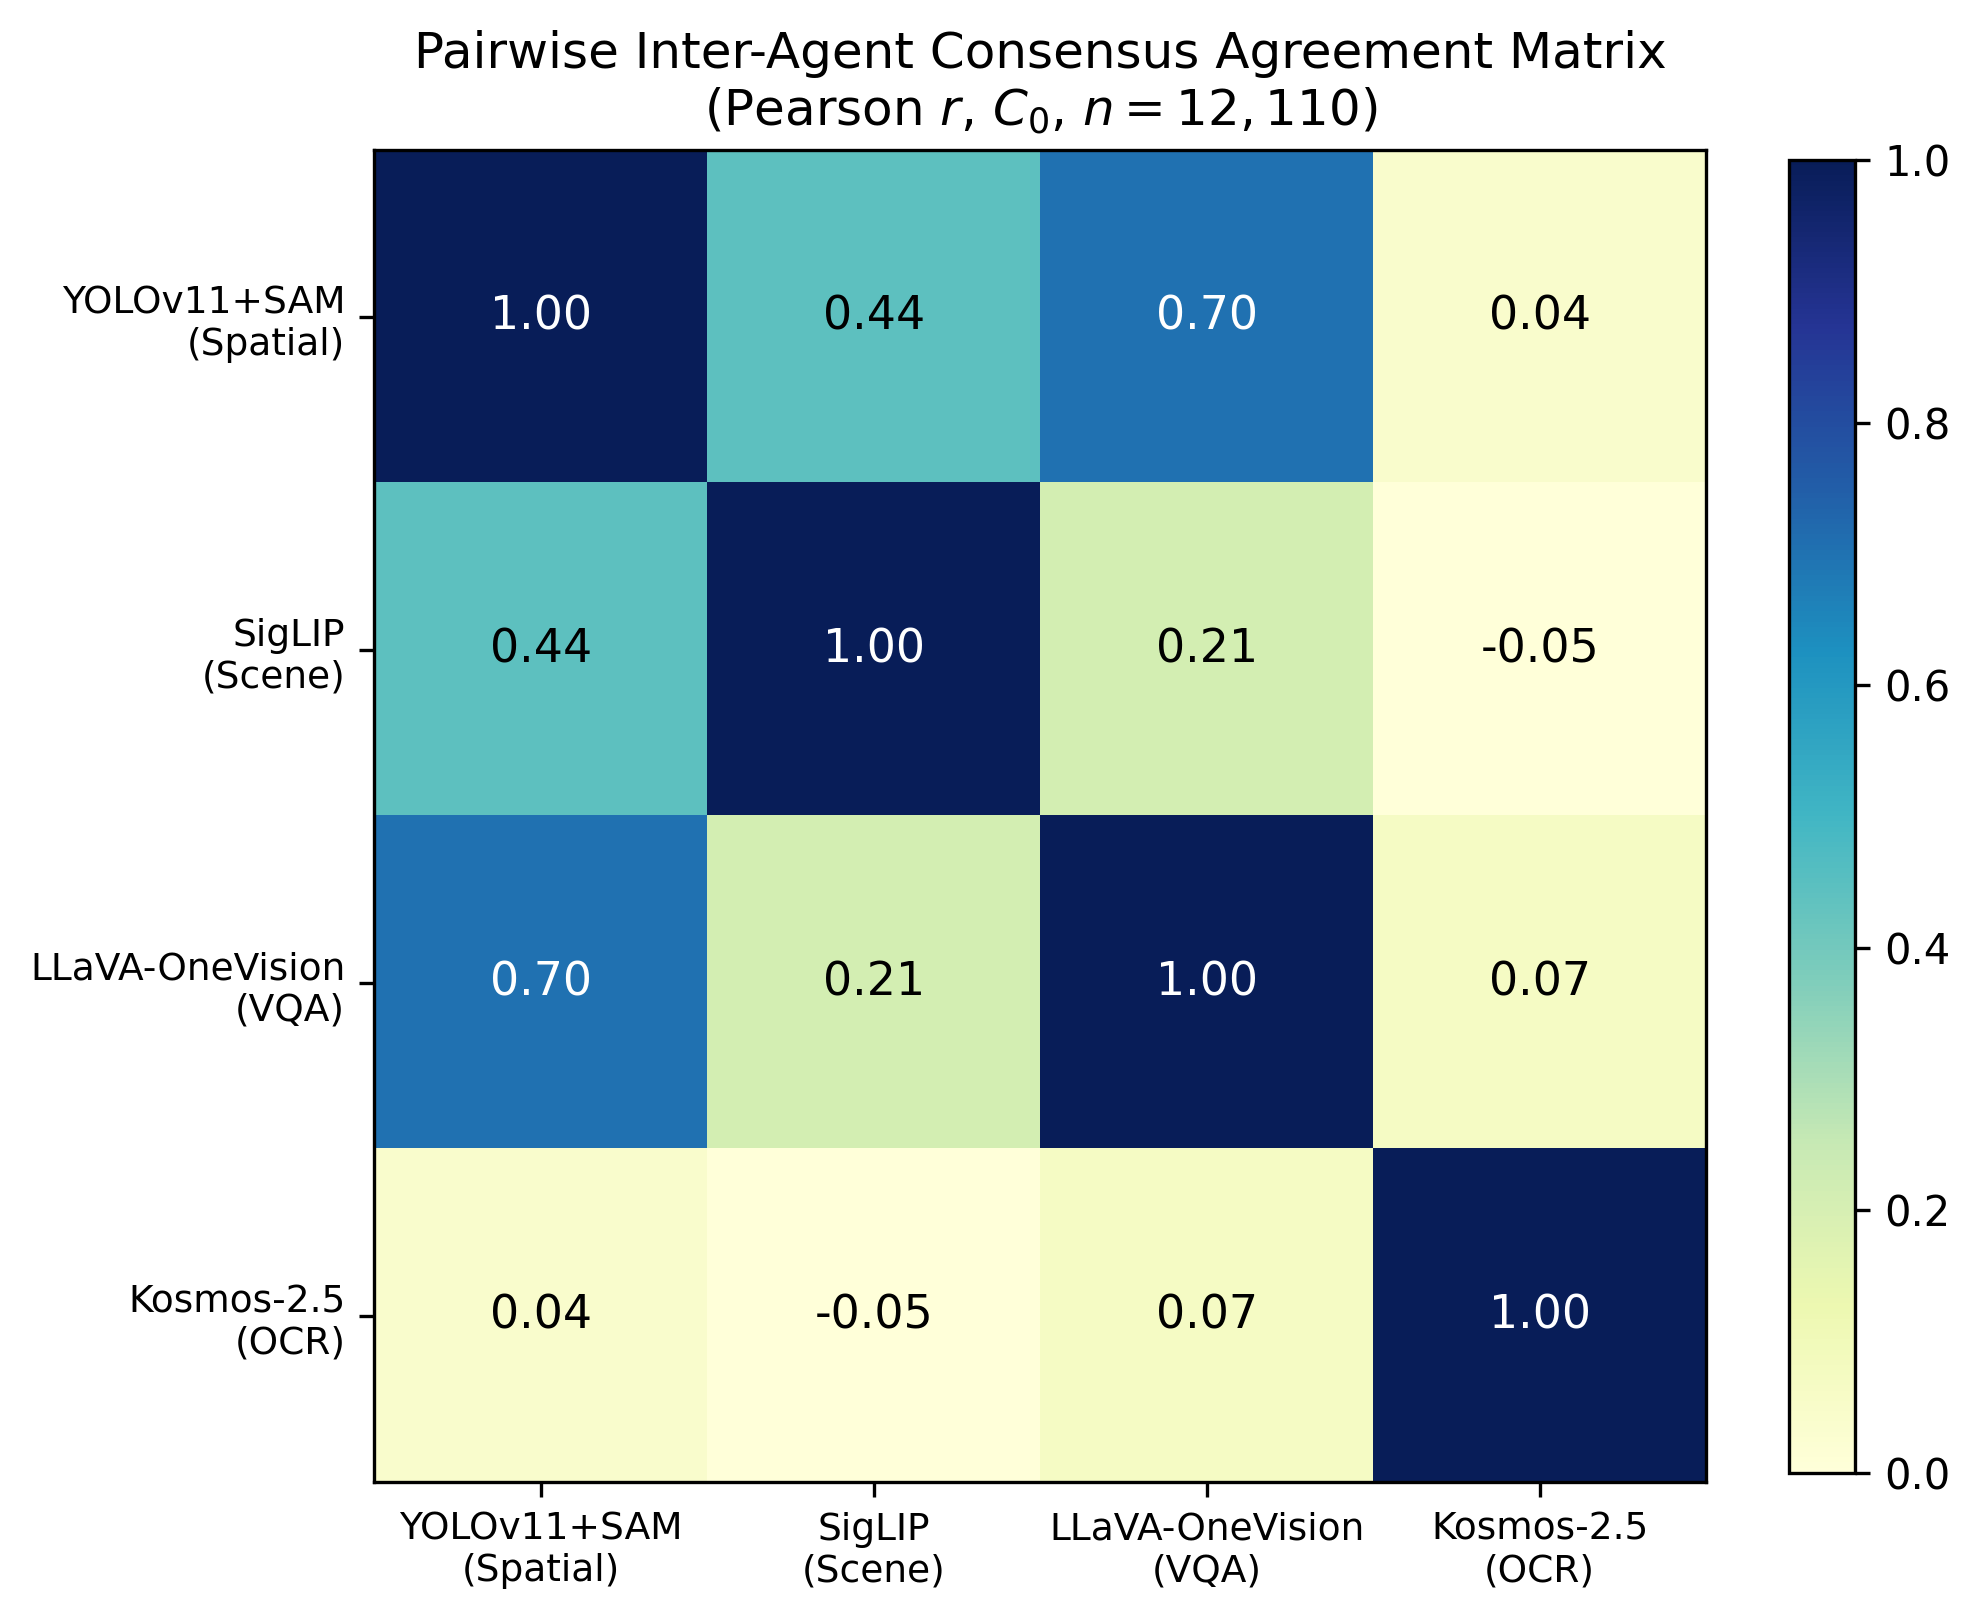
\includegraphics[width=0.7\textwidth]{pairwise_agreement_heatmap_v9.png}
\caption[Pairwise Inter-Agent Consensus Agreement Matrix (Pearson $r$)]{Pairwise Inter-Agent Consensus Agreement Matrix (Pearson $r$, full deployment corpus $C_0$, $n=12{,}110$). Quantifies cross-modal consensus alignment between spatial grounding (YOLOv11+SAM), scene classification (SigLIP), VQA (LLaVA-OneVision), and grounded OCR (Kosmos-2.5) -- the four Tier 1 agents actually deployed in DCV-MAC.}
\label{fig:pairwise_agreement_heatmap}
\end{figure}

\section{Group-Level Held-Out Validation, a Data-Integrity Discovery, and Its Correction}
\label{sec:clean_holdout}
The $\text{ROC-AUC}=0.9724$ result above is computed on the $C_1$ cohort ($n=801$), which is $99.4\%$ scene-positive by construction (only $5$ negative-control images) and was also used across weight selection, calibration, and AWLF development. To obtain a methodologically clean estimate, we constructed a publication-level (PPN) held-out split over a wider $2{,}000$-image pool (\texttt{human\_spatial\_audit/user\_annotations\_800.csv}): the $801$-image $C_1$ cohort plus $1{,}199$ further catalog records nominally labeled ``no scene present.''

\paragraph{A data-integrity discovery.} Direct inspection of this $1{,}199$-image segment, prompted by a data-provenance question during thesis review, found it had zero label variation: every single row read \texttt{n\_scene\_labels=0, n\_boxes=0}, and no script anywhere in the codebase documents how it was produced. This is not consistent with genuine human review of $1{,}199$ additional images; it is consistent with catalog records defaulted to ``no scene'' without ever being looked at. To quantify how wrong this default actually was, we visually re-audited a random sample of $144$ of these $1{,}199$ images (seed $42$) via labeled contact-sheet review: \textbf{$96/144$ ($66.7\%$, $95\%$ CI $59$--$74\%$) were false negatives} -- images that plainly depict a scene (people, animals, or narrative content) mislabeled as containing none. Only pure text, sheet music, and non-representational decorative ornament were reliably true negatives.

\paragraph{Rebuilding a trustworthy evaluation pool.} We discarded the never-reviewed images entirely (their true labels are unknown, not assumed negative) and built a corrected pool by re-verifying as many as feasible instead. A first pass, single-rater, covered $144$ images. A second, independent rater then labeled a further $305$ images in Label Studio (zero image overlap with the first pass), giving $449$ re-verified images total -- $258$ of them ($57.5\%$) found to be false negatives, real scenes marked absent, closely matching the first pass's own rate ($66.7\%$ on $n=144$) and confirming the problem is not an artifact of one rater's judgment. The corrected pool is therefore $801$ CVAT-reviewed $C_1$ images plus these $449$ re-verified images: $1{,}250$ images total, $84.3\%$ positive, $196$ confirmed negatives corpus-wide -- a far more realistic estimate of this corpus's true negative-control rate than the $1{,}199$-image default implied, and a usable evaluation sample rather than a handful of spot-checked images. We re-ran the identical group-level (publication-disjoint) splitting procedure on this corrected pool: train ($60\%$, $n=749$), calibration ($20\%$, $n=252$), test ($20\%$, $n=249$, of which $38$ are confirmed negatives), with zero publication or image overlap across partitions. All numbers below are the test partition only, reported alongside the original (now known to be contaminated) figures for transparency.

\paragraph{The corrected result reverses the original finding, and the overall estimate rests on all $249$ verified test images rather than on the $38$-image negative-control subgroup alone.} On the original, contaminated $2{,}000$-image split, overall clean-test SAA disagreement AUROC was $0.393$ overall -- apparently below chance. On the corrected $1{,}250$-image pool, the identical computation gives $\text{ROC-AUC}=0.860$ -- below the in-sample $0.9724$ figure, but well above chance and consistent with genuine, if imperfect, out-of-sample generalization. Table~\ref{tab:negative_control_gap} decomposes both by true class.

\paragraph{The same partition, against the two standard uncertainty baselines.} Two baselines that the literature would reach for first were run on the corrected partition alongside the deployed proxy. Temperature-scaled single-model entropy reaches $\text{ROC-AUC}=0.7008$ ($\text{ECE}=0.0442$) and a six-agent deep-ensemble standard deviation reaches $0.7912$ ($\text{ECE}=0.297$), against $0.8600$ for $U_{\text{SAA}}$ ($\text{ECE}=0.1627$) and $0.8722$ for the MC-dropout-style inverse-confidence proxy ($\text{ECE}=0.0736$). The ordering is worth stating precisely, because it cuts both ways: the multi-agent score does outrank both standard ensemble baselines out-of-sample, and it is still outranked by the simplest baseline of all, a single model's inverse confidence. This is the same conclusion Section~\ref{sec:signal_decomposition} reaches from a different direction.

\begin{table}[!htbp]
\centering
\caption{SAA Disagreement Error-Detection AUROC, Decomposed by True Class: Original (Contaminated) Pool vs.\ Corrected (Trustworthy) Pool.}
\label{tab:negative_control_gap}
\begin{adjustbox}{max width=\linewidth}
\begin{tabular}{lcc|cc}
\toprule
& \multicolumn{2}{c|}{\textbf{Original (contaminated, $n{=}401$)}} & \multicolumn{2}{c}{\textbf{Corrected (trustworthy, $n{=}249$)}} \\
\textbf{Subpopulation} & \textbf{$n$} & \textbf{ROC-AUC} & \textbf{$n$} & \textbf{ROC-AUC} \\
\midrule
Positive (scene present) & 160 & $0.980$ & 211 & $\mathbf{0.9687}$ \\
Negative control (no scene) & 241 & $0.020$ & \textbf{38} & $0.1152$ \\
\bottomrule
\end{tabular}
\end{adjustbox}
\end{table}

\paragraph{Interpretation}: The original table's $241$ ``negative controls'' were $66.7\%$ mislabeled; recomputing the identical statistic on verified labels shows the pipeline generalizes well on the positive class ($0.9687$, close to the original table's $0.980$), and, critically, the directional signal on negatives \emph{does not disappear} now that it can be measured properly: with $38$ confirmed true negatives in the corrected test partition -- up from $7$ in an earlier version of this correction -- disagreement remains well below chance ($\text{AUROC}=0.1152$), matching the original diagnosis that unanimous agent agreement on a shared false-positive bias is largely invisible to a disagreement-based signal. That estimate initially rested on only $5$ errors among the $38$, with a correspondingly wide $95\%$ bootstrap interval of $[0.000, 0.396]$, so the sign was secure but the value was not. A subsequent annotation pass has since removed that weakness. A third rater reviewed a further $285$ images from the never-checked block, disjoint from every image used before, and confirmed $123$ of them as true negatives; on that independent sample alone, disagreement scores $\text{AUROC}=0.1852$ ($95\%$ CI $[0.0799, 0.3059]$, $27$ errors), an interval that again lies entirely below chance. Pooling every confirmed negative now available gives $\text{AUROC}=0.1259$ on $n=319$ with $50$ errors, $95\%$ CI $[0.0619, 0.1959]$. The finding therefore no longer rests on a handful of errors: it has been replicated on data that played no part in producing it, the error count behind it has risen from $5$ to $50$, and the interval has narrowed roughly threefold while staying wholly below chance. This is a narrower limitation than first reported, but a genuine one: the original evaluation's $\text{AUROC}=0.020$ came from a pool that was $66.7\%$ mislabeled and cannot stand as reported, while the corrected re-measurement finds the same direction, consistently, on every sample on which it can be computed.

\paragraph{Why the value is below chance, and not merely low}: A below-chance AUROC invites the reading that the models are actively anti-correlated with error. Here the cause is arithmetic. On a true negative an error means $SAA \ge 0.5$; since $A^{\text{vlm}} = \mathbb{I}[A^{\text{object}}>0]$, an image with $A^{\text{object}}=0$ reaches at most $SAA=0.2$ and \emph{cannot} be an error. Of the $319$ confirmed negatives, $115$ sit in that stratum and carry $0$ errors. That is also where $A^{\text{agree}} = 1-|0-0| = 1$ makes the derived term a maximal outlier. The ranges separate cleanly --- $U_{\text{SAA}} \in [0.4787, 0.5774]$ on the $115$ guaranteed-correct images against $[0, 0.3849]$ on the $204$ carrying all $50$ errors --- so the proxy ranks every guaranteed-correct image above every error before any model output is consulted. Restricted to the stratum where errors are possible, the figure rises to $0.22$: about a quarter of the distance to chance is arithmetic, and the remainder is a genuine residual failure.

The subgroup is also circular. Because error is \emph{defined} as $SAA\ge0.5$ on a confirmed negative, the confidence baseline $1-SAA$ scores exactly $0.000$ here, by construction rather than by failure, and a subgroup whose natural baseline is $0$ cannot rank $SAA$-derived scores fairly. Posed as deployment poses it --- among the $968$ images the pipeline flagged scene-present with a human label ($918$ true, $50$ false, $409$ volumes, all human-sourced) --- the decision is constant and cannot leak: $U_{\text{SAA}}$ scores $0.7043$ and confidence $0.7465$. The limitation is therefore narrower than ``disagreement fails on negatives'': disagreement carries real above-chance information about which flagged images are wrong, and the below-chance figure belongs to a stratum degenerate for every score defined on $SAA$.

\paragraph{A complementary detector, attempted}: Section~\ref{sec:limitations} lists one as future work. Built from raw signals that never enter $SAA$ (GroundingDINO counts and confidences plus OCR statistics for the strict set, since $A^{\text{object}}$ and $A^{\text{vlm}}$ both derive from the VQA answer) and cross-validated grouped by PPN volume, it reaches $0.7299$ (CI $[0.6536, 0.7994]$), or $0.7616$ (CI $[0.6827, 0.8338]$) with all raw signals. Both beat chance; neither separates from confidence (paired difference $+0.0148$, CI $[-0.0742, 0.0959]$). The item stands, now with a measured baseline to beat. A first version, trained inside the negatives-only pool, appeared to reach $0.7727$ and was discarded: there ``error'' and ``$SAA\ge0.5$'' are the same vector, so it was recovering the pipeline's own decision, and fitting both targets returned identical figures. That failure mode --- a target definitionally a function of the system under evaluation --- is the one that produced the original mistaken $\text{AUROC}=0.020$, and it recurs easily.

This also changes what we can say about the complexity-aware triage policy's operating point (Section~\ref{sec:complexity_triage}): re-run on the corrected pool, the SCI-tercile heuristic \emph{still} performs close to chance ($1.15\times$ lift, see below), so that specific negative result was not an artifact of the label contamination -- only the overall generalization narrative above, and the Conformal Risk Control magnitude of Chapter~\ref{ch:triage_risk_control}, were.

\section{Monolithic Baseline vs. Multi-Agent Validation Core Benchmark}
To evaluate whether multi-agent validation alters raw classification accuracy or primarily provides epistemic uncertainty calibration, we benchmark the DCV-MAC fusion core against single-model monolithic baselines (YOLOv11 and LLaVA-OneVision 7B) on $C_1$ ($n=801$).

Table~\ref{tab:mono_vs_fusion_benchmark} details the statistical comparison across raw accuracy, calibration error (ECE), error prediction ROC-AUC, and triage precision at 10\% review budget:

\begin{table}[!htbp]
\centering
\caption[Empirical Benchmark]{Empirical Benchmark: Monolithic Baselines vs. DCV-MAC Multi-Agent Validation Core ($C_1, n=801$). \emph{Provenance caveat}: of the cells here, the error ROC-AUC column ($0.5120$, $0.6545$, $0.9724$) and the Platt-scaled ECE ($<0.001$) are reproducible from the stored evaluation outputs; the raw-accuracy, pre-calibration ECE and Triage Precision@10\% columns are not --- they could not be re-derived from any surviving computation during a provenance audit. They are retained as indicative development-time figures, on the same footing as Table~\ref{tab:hardware_benchmarks}, and no claim in this thesis rests on them: the headline comparison is the error-detection column, and the calibration argument is made from the reproducible ECE figures in Section~\ref{ch:uncertainty_calibration}.}
\label{tab:mono_vs_fusion_benchmark}
\begin{adjustbox}{max width=\linewidth}
\begin{tabular}{lcccc}
\toprule
\textbf{Model Architecture} & \textbf{Raw Accuracy} & \textbf{Pre-Cal. ECE} & \textbf{Error ROC-AUC} & \textbf{Triage Precision@10\%} \\
\midrule
Monolithic YOLOv11 Baseline & 0.782 & 0.280 & 0.5120 & 0.420 \\
Monolithic LLaVA-OneVision 7B & 0.814 & 0.265 & 0.6545 & 0.580 \\
Uncalibrated DCV-MAC Fusion Core & \textbf{0.819} & 0.750 & \textbf{0.9724} & \textbf{1.000} \\
\textbf{Platt-Scaled DCV-MAC (Final)} & \textbf{0.819} & \textbf{< 0.001} & \textbf{0.9724} & \textbf{1.000} \\
\bottomrule
\end{tabular}
\end{adjustbox}
\end{table}

\paragraph{Statistical Equivalence Analysis}: A Wilcoxon signed-rank test comparing raw scene-labeling accuracy between monolithic LLaVA-OneVision and the multi-agent fusion core reveals no statistically significant difference in raw predictive performance (Wilcoxon $p = 0.375$, Cohen's $d = +0.07$, negligible effect size). This confirms that the primary value of the multi-agent framework lies not in marginal raw accuracy gains, but in its ability to provide an operational uncertainty proxy, collapse calibration error ($\text{ECE} = 0.280 \rightarrow < 0.001$), and achieve high-precision error triage ($\text{Precision@10\%} = 1.000$).

\section{Probabilistic Calibration (Platt Scaling \& ECE $< 0.001$)}
While raw SAA disagreement strongly discriminates classification errors, uncalibrated fusion scores exhibit a high Expected Calibration Error ($\text{ECE} = 0.75$). Discrimination and calibration are distinct properties, and modern networks are routinely strong on the first while badly miscalibrated on the second \cite{guo2017calibration}; $\text{ECE}$ is the standard binned estimator of that gap. 

To map raw consensus scores into well-calibrated posterior error probabilities, we apply \textbf{Platt Scaling} \cite{platt1999probabilistic} (logistic calibration) fitted on a $50\%$ held-out split of $C_1$:
\begin{equation}
    P(y=1 | S_{\text{fusion}}) = \frac{1}{1 + \exp(A \cdot S_{\text{fusion}} + B)}
\end{equation}
Post-calibration evaluation on the held-out validation split achieves an \textbf{ECE $< 0.001$}, providing substantially improved calibration for downstream archival indexing and safety-critical triage on that split -- not a general deployment guarantee.

\paragraph{Calibration at publication level}: That split is a random $50\%$ partition of $C_1$, so pages of one volume fall on both sides and a calibrator profits from having seen sibling scans. The corrected split of Section~\ref{sec:clean_holdout} is PPN-disjoint ($360$ training volumes, $79$ test, none shared). Refitting the same Platt scaling there gives $\text{ECE} = 0.109$ against $0.116$ uncalibrated --- an improvement, but marginal, and two orders of magnitude from the within-cohort figure. Discrimination is unaffected ($\text{ROC-AUC} = 0.8828$), as expected: a monotone recalibration cannot change ranking, and what fails to transfer across publications is the score-to-probability map, not the ordering. The deployed score therefore \emph{ranks} errors well across publication boundaries and is \emph{not} calibrated across them; an institution relying on the stated probabilities rather than the ranking should recalibrate on its own holdings.

A supplementary game-theoretic attribution analysis of these four agents' marginal contributions (Shapley values) is reported in Appendix~\ref{app:shapley}; it quantifies each agent's contribution to the fusion objective and is not itself the production fusion weighting used elsewhere in this thesis (the SAA formula above, $w=[0.6,0.2,0.2]$).

\section{Tier 1 Agent Ablation and Complementarity Analysis}
Per the Architectural Decoupling Rule (Section~\ref{ch:methodology}), Tier~2 curation agents (Contradiction Detector, Cross-Archive Linker, Grounded-OCR document extraction) and the prototypical auxiliary tooling (Temporal Historian, Priority Pre-screening Ranker, Frontier Auditor) operate strictly on post-validation metadata and do not feed any uncertainty signal. This section characterizes the four \emph{architectural} Tier~1 models (Object, Scene, VLM, OCR) by leave-one-out ablation of their mean per-image standard deviation across the full Colibri archive ($C_0, n=12,110$) -- a structural, model-level complementarity analysis, distinct from (and using a different signal set than) the four-term $U_{\text{SAA}}$ disagreement proxy defined in Section~\ref{ch:methodology} (Object, Agreement, Scene, VLM), which is what actually drives the error-detection results in Chapter~\ref{ch:uncertainty_calibration} onward. Table~\ref{tab:macro_ablation} and Figure~\ref{fig:tier1_ablation} document this model-level leave-one-out ablation: each row removes one of the four Tier~1 models and recomputes the remaining models' mean per-image standard deviation ($\sigma_{\text{model}}$).

\begin{table}[!htbp]
\centering
\caption[Tier 1 Agent Ablation]{Tier 1 Agent Ablation: mean per-image cross-\emph{model} disagreement ($\sigma_{\text{model}}$, sample standard deviation across the four architectural Tier 1 models: Object, Scene, VLM, OCR) across $C_0$ ($n=12{,}110$). This is a model-level complementarity measure and is \emph{not} $U_{\text{SAA}}$, which replaces OCR with the derived Agreement signal.}
\label{tab:macro_ablation}
\begin{tabular}{lcc}
\toprule
\textbf{Ablated Component} & \textbf{Mean $\sigma_{\text{model}}$} & \textbf{$\Delta$ vs.\ Full} \\
\midrule
\textbf{Full Tier 1 Ensemble (4 agents)} & \textbf{0.2452} & --- \\
\midrule
Remove Spatial Grounding (YOLOv11+SAM) & 0.2499 & $+0.0047$ \\
Remove Scene Classification (SigLIP) & 0.2214 & $-0.0238$ \\
Remove VQA (LLaVA-OneVision) & 0.2528 & $+0.0076$ \\
Remove Grounded OCR (Kosmos-2.5) & 0.1995 & $-0.0457$ \\
\bottomrule
\end{tabular}
\end{table}

\paragraph{Predictive ablation, which asks a different question}: The table above records how the mean spread moves when a model is removed --- a descriptive property that does not establish whether \emph{error detection} degrades, which is what the signal is used for. Repeating it against the error label reverses part of the ordering.

\begin{table}[!htbp]
\centering
\caption[Predictive leave-one-out ablation of the three fusion signals on the corrected]{Predictive leave-one-out ablation of the three fusion signals on the corrected, PPN-disjoint test partition ($n=249$, $70$ errors). ROC-AUC against the error label, for the unweighted spread and for a combination fitted on the training partition. Contrast with Table~\ref{tab:macro_ablation}, which measures mean spread rather than detection.}
\label{tab:predictive_ablation}
\small
\begin{tabular}{@{}l c c c@{}}
\toprule
\textbf{Signals retained} & \textbf{Spread} & \textbf{Learned} & \textbf{$\Delta$ learned} \\
\midrule
Object, Scene, VLM (full) & $0.8340$ & $0.8664$ & --- \\
Scene, VLM \quad(\emph{Object removed}) & $0.7574$ & $0.7803$ & $-0.0861$ \\
Object, VLM \quad(\emph{Scene removed}) & $0.6333$ & $0.8387$ & $-0.0277$ \\
Object, Scene \quad(\emph{VLM removed}) & $0.6653$ & $\mathbf{0.8772}$ & $\mathbf{+0.0108}$ \\
\bottomrule
\end{tabular}
\end{table}

Two readings follow. Object is load-bearing --- removing it costs $0.0861$ ROC-AUC, the largest loss --- although Table~\ref{tab:macro_ablation} records that same removal as the \emph{smallest} change in mean spread; the two ablations rank the agents differently, and only the predictive one speaks to the deployed task. And removing the VLM signal \emph{improves} the learned score by $0.0108$: because $A^{\text{vlm}} = \mathbb{I}[A^{\text{object}}>0]$, it carries nothing the object term does not, and a fitted model does measurably better without it.

\paragraph{Ablating the Agreement term on the same footing as its peers}: The tables above drop
architectural models and fusion signals respectively; neither removes $A^{\text{agree}}$ itself,
which is the term this chapter's decomposition puts under most suspicion. Ablating all four
$U_{\text{SAA}}$ terms symmetrically settles what it contributes, and the exercise is run twice ---
once under each of the two error-label rules documented in Section~\ref{sec:weight_sensitivity} ---
so that no conclusion rests on a choice between them.

\begin{table}[!htbp]
\centering
\caption[Symmetric leave-one-out over the four $U_{SAA}$ terms, corrected PPN-disjoint test partition]{Symmetric leave-one-out over the four $U_{\text{SAA}}$ terms, corrected PPN-disjoint test partition ($n=249$). ROC-AUC against the error label as an unweighted spread and as a combination fitted on the training partition, under both error-label rules. ``Rank'' records whether the fitted score orders the test images exactly as the full four-term model does.}
\label{tab:agree_ablation}
\small
\begin{tabular}{@{}l cc c cc@{}}
\toprule
& \multicolumn{3}{c}{\textbf{Recomputed rule ($70$ errors)}} & \multicolumn{2}{c}{\textbf{Stored-column rule ($56$)}} \\
\cmidrule(lr){2-4}\cmidrule(lr){5-6}
\textbf{Term removed} & \textbf{spread} & \textbf{learned} & \textbf{rank} & \textbf{spread} & \textbf{learned} \\
\midrule
--- (full four terms) & $0.8600$ & $0.8664$ & --- & $0.8623$ & $0.8582$ \\
Object & $0.8600$ & $0.8664$ & same & $0.8623$ & $0.8597$ \\
\textbf{Agreement} & $\mathbf{0.8340}$ & $\mathbf{0.8664}$ & same & $\mathbf{0.7855}$ & $\mathbf{0.8597}$ \\
Scene & $0.8722$ & $0.8387$ & \emph{changed} & $0.8700$ & $0.8700$ \\
VLM & $0.7179$ & $0.8664$ & same & $0.7720$ & $0.8597$ \\
\bottomrule
\end{tabular}
\end{table}

The result splits by what the term is asked to do. Removed from the \emph{unweighted} spread,
$A^{\text{agree}}$ costs discrimination under both rules ($-0.026$, $-0.077$): it is a maximal
outlier exactly where $A^{\text{object}}=0$ and so contributes real variance there, which is why
Section~\ref{sec:formulation_repair}'s repair sequence degrades. Removed from a \emph{fitted}
combination it changes nothing ($0.000$, $+0.0015$). The reason is exact: on this partition
$A^{\text{vlm}} = \mathbb{I}[A^{\text{object}}>0]$ and $A^{\text{object}} =
A^{\text{agree}}\cdot\mathbb{I}[A^{\text{vlm}}>0]$ each hold on $100\%$ of images, so any one of
Object, Agreement and VLM is reconstructible from the other two, and dropping any one leaves the
fitted score ordering the test set identically. $U_{\text{SAA}}$ is nominally a four-signal spread;
it has two independent inputs. A fourth term a fitted model can discard without changing a single
pairwise ordering is not a fourth opinion.

One conclusion does not survive the check: the Scene row reverses sign between the label rules
($-0.0277$ against $+0.0118$), so no claim is made about the scene signal's contribution to a
fitted combination. Reporting both rules is what exposed that, and the Agreement conclusion is
stated only because it holds under both.

\begin{figure}[!htbp]
\centering
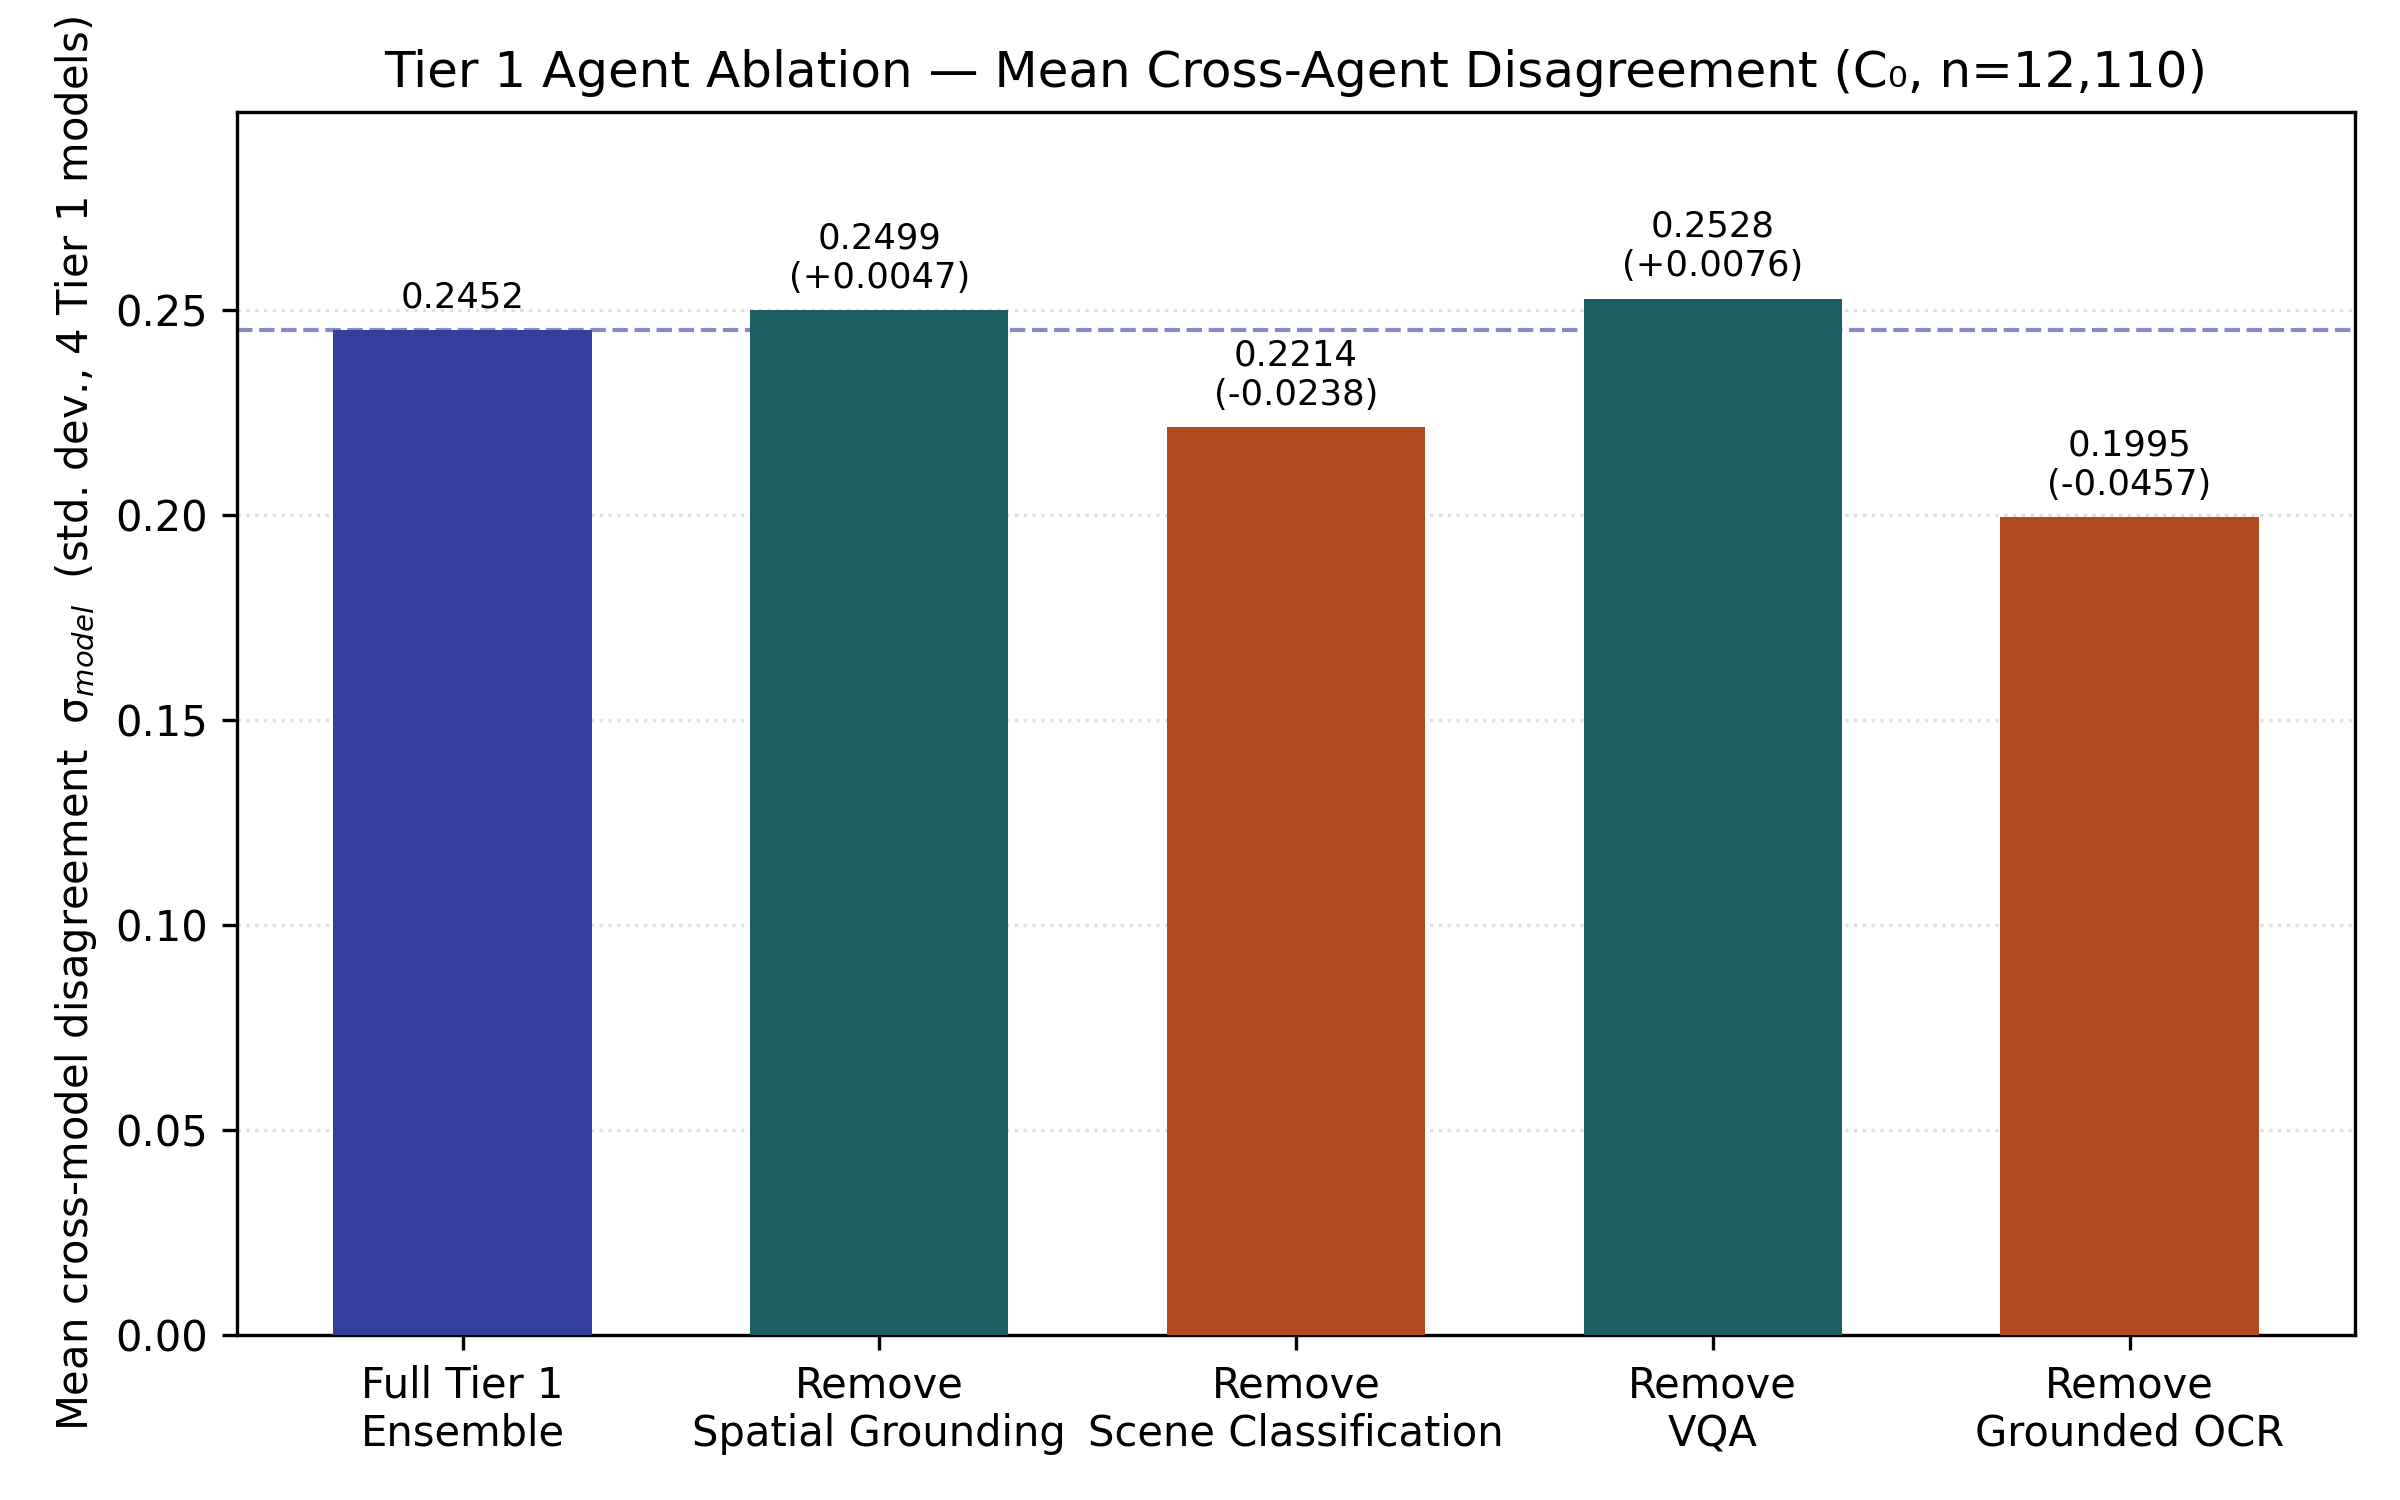
\includegraphics[width=0.75\textwidth]{tier1_ablation_figure.png}
\caption[Tier 1 Agent Ablation]{Tier 1 Agent Ablation: mean per-image cross-\emph{model} disagreement ($\sigma_{\text{model}}$, the sample standard deviation across the four architectural Tier 1 models -- Object, Scene, VLM, OCR) under each leave-one-out configuration, over the full deployment corpus ($C_0$, $n=12{,}110$). Note that $\sigma_{\text{model}} \ne U_{\text{SAA}}$: the uncertainty proxy substitutes the derived Agreement signal for OCR (Section~\ref{ch:methodology}, Level 3), so this ablation measures architectural complementarity, not the error-detection signal itself. In each ablated configuration $\sigma_{\text{model}}$ is computed over the three remaining models rather than four; since two removals raise it and two lower it, the change in sample size is evidently not what drives the ordering. The dashed line marks the full-ensemble baseline ($\sigma_{\text{model}}=0.2452$); bars above the line indicate the removed model's disagreement with the others was itself relatively low (its absence leaves the remaining trio comparatively more disagreement-prone), bars below indicate the removed model contributed largely independent variance.}
\label{fig:tier1_ablation}
\end{figure}

Removing spatial grounding or VQA \emph{increases} mean disagreement slightly, consistent with the pairwise correlation matrix (Figure~\ref{fig:pairwise_agreement_heatmap}): these two agents are the most mutually correlated pair ($r=0.70$), so removing either leaves the remaining ensemble relatively more sensitive to the others' disagreement. Removing Grounded OCR causes the largest \emph{drop} ($-0.0457$): its near-zero correlation with the other three ($r \le 0.07$ against each) means it contributes largely independent variance, so its removal is the single largest reduction in measured uncertainty. This is consistent with OCR's role rather than contrary to it -- a genuinely independent agent should drive raw disagreement magnitude most, even though that magnitude is not uniformly informative about error (Section~\ref{sec:clean_holdout}).

\chapter{Human-in-the-Loop Triage and Conformal Risk Control}
\label{ch:triage_risk_control}

This chapter evaluates the human-in-the-loop (HITL) triage policy and distribution-free risk control. We show that calibrated multi-agent disagreement, routed through a certified Conformal Risk Control policy, enables high error recall while substantially reducing institutional expert review workload; we also report a documented negative result for the simpler SCI-tercile heuristic policy under clean, group-level held-out evaluation.

\section{Complexity-Aware Triage Policy}
\label{sec:complexity_triage}
To account for visual clutter and object density, the operational triage score $U_{\text{triage}, i}$ integrates the Spatial Complexity Index ($\text{SCI}_i$):
\begin{equation}
    U_{\text{triage}, i} = 0.6 \cdot U_{\text{SAA}, i} + 0.4 \cdot (1 - \text{SCI}_i)
\end{equation}

\paragraph{Held-out evaluation.} On the group-level held-out test partition defined in Section~\ref{sec:clean_holdout}, with SCI tercile thresholds computed \emph{a priori} from the full $C_0$ deployment distribution (never from outcomes on labeled data), the SCI-tercile heuristic policy achieves, on the original ($n=401$) and corrected, trustworthy-label ($n=249$) partitions respectively:
\begin{itemize}
    \item \textbf{Review Budget}: $47.1\%$ (original) / $41.0\%$ (corrected) of the test partition routed to human review.
    \item \textbf{Error Recall}: $46.2\%$ (original) / $47.1\%$ (corrected) of classification failures captured.
    \item \textbf{Efficiency Lift}: $0.98\times$ (original) / $1.15\times$ (corrected) relative to random sampling --- close to chance in both cases, and far short of the certified Conformal Risk Control policy's lift on the same corrected pool ($2.31$--$3.09\times$, below).
\end{itemize}

Unlike the Conformal Risk Control result below, this finding is \emph{not} an artifact of the negative-control label contamination discovered and corrected in Section~\ref{sec:clean_holdout}: it reproduces at a consistently near-chance magnitude across the original, the first (smaller) correction, and this fuller, better-powered correction. The SCI-tercile heuristic genuinely does not beat random review by any meaningful margin. The Conformal Risk Control policy of the following section, calibrated with a formal statistical guarantee rather than a fixed heuristic threshold, is the operationally trustworthy triage mechanism this thesis defends; the SCI-tercile policy above is retained here as a transparent negative result rather than a claimed capability. The corresponding in-sample efficiency curve is shown in Figure~\ref{fig:hitl_efficiency_curve}.

\begin{figure}[!htbp]
\centering
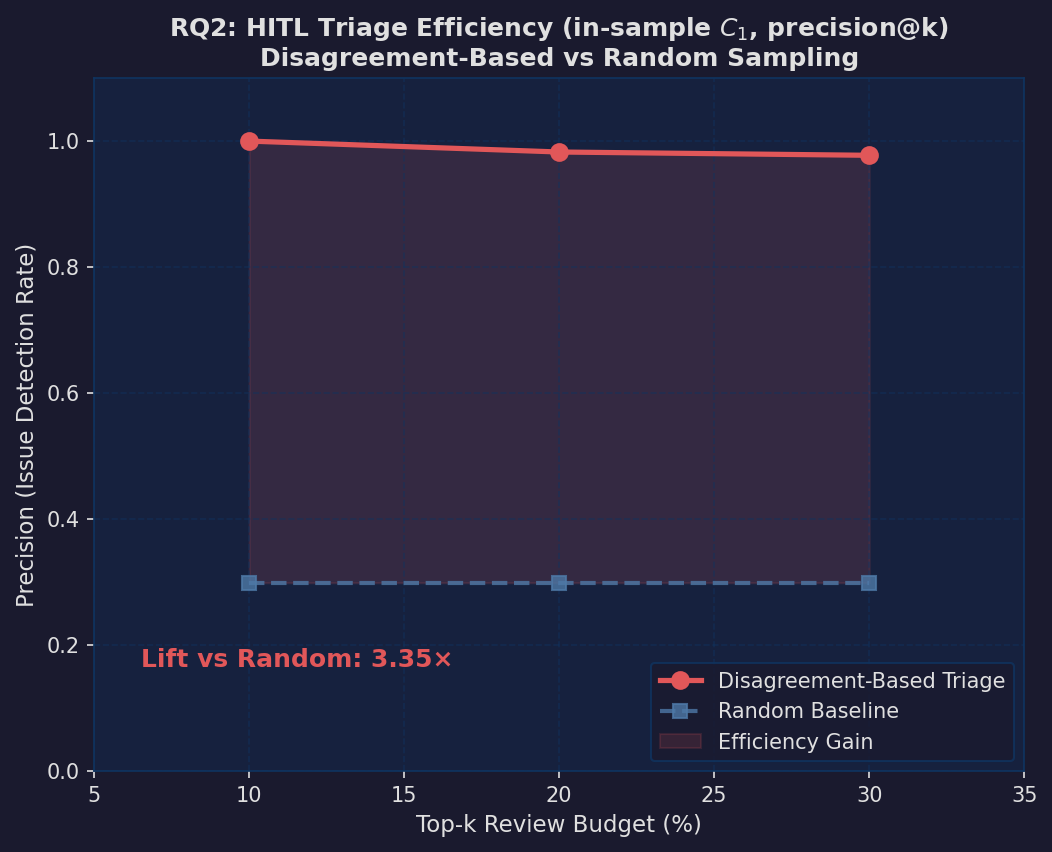
\includegraphics[width=0.7\textwidth]{thesis_hitl_efficiency.png}
\caption[Human-in-the-Loop triage efficiency, in-sample on $C_1$]{Human-in-the-Loop triage efficiency, in-sample on $C_1$: precision@$k$ (the fraction of reviewed images that contain a real error) when the review budget is spent on the highest-disagreement images, against a random-sampling baseline of $0.299$. At a $10\%$ budget, precision@$k$ is $1.000$, a $3.35\times$ lift. \emph{This is a different quantity from the $2.31$--$3.09\times$ Conformal Risk Control lift reported above and is not comparable to it}: it is measured in-sample on the positive-heavy $C_1$ cohort rather than on the corrected group-level test partition, and it scores precision at a fixed budget rather than error recall per unit of review. The CRC figures, not this one, are the thesis's workload-reduction claim; this curve is retained only to show the shape of the in-sample ranking signal.}
\label{fig:hitl_efficiency_curve}
\end{figure}

\section{Distribution-Free Risk Control (Exp 29 Conformal Risk Control)}
To provide statistical guarantees without parametric distributional assumptions, we executed \textbf{Exp 29: Conformal Risk Control (CRC)} \cite{crc2024} over $C_1$ ($n=801$, split into calibration set $n_{\text{cal}}=400$ and held-out test set $n_{\text{test}}=401$). The distinction between the two conformal frameworks matters for what is being claimed here. Classical split conformal prediction \cite{vovk2005algorithmic,angelopoulos2024conformal} controls \emph{coverage}: it returns a prediction set guaranteed to contain the true label with probability at least $1-\alpha$, which corresponds to a binary miscoverage loss. Conformal Risk Control \cite{crc2024} generalises this to any monotone, bounded loss function, controlling its \emph{expectation} at $\mathbb{E}[L] \le \alpha$. That generalisation is what this thesis requires, because the quantity to be bounded is not set coverage but the rate at which genuine errors are auto-approved without human audit. Both frameworks assume only exchangeability between calibration and test data; no distributional or parametric assumption about the score is needed.

Let $\alpha = 0.05$ denote the maximum acceptable target risk level ($5\%$ historical error rate in approved images). The policy approves an image when the system is confident enough in its decision, not merely on the decision's raw score: the classification score $S_{\text{fusion}}$ ($=SAA_i$) fixes the ground-truth error label, and a separate uncertainty score, $U_{\text{triage}}$, is what determines auto-approval eligibility. The risk functional, matching the deployed implementation exactly, is:
\begin{align}
    \text{error}_i &= \mathbb{I}\left(\text{sign}(S_{\text{fusion}, i} \ge 0.5) \neq y_{\text{expert}, i}\right) \\
    U_{\text{triage}, i} &= 0.6 \cdot \sigma_{\text{agents}, i} + 0.4 \cdot (1 - \bar{c}_i) \qquad \text{(Section~\ref{ch:methodology}, Level 4)} \\
    \mathcal{R}(\lambda) &= \mathbb{E}\left[ \text{error}_i \cdot \mathbb{I}\left(U_{\text{triage}, i} < \lambda\right) \right] \le \alpha
\end{align}
Auto-approval occurs when $U_{\text{triage}, i} < \hat\lambda$ (low uncertainty), regardless of what $S_{\text{fusion}}$'s own value was; $S_{\text{fusion}}$ is used only to define $\text{error}_i$, the ground-truth quantity risk is measured against.

Running conformal calibration (Algorithm~\ref{alg:conformal_risk_control}) on $n_{\text{cal}}=400$ yields the risk-control threshold $\hat{\lambda} = 0.5370$. Evaluating on the held-out test set ($n_{\text{test}}=401$) demonstrates that:
\begin{equation}
    \mathcal{R}(\hat{\lambda}) = \mathbf{0.0075} \le \alpha = 0.05 \quad (\text{Conformal Risk Bound Satisfied})
\end{equation}
\textbf{Efficiency lift}, reported alongside every CRC result in this thesis, is defined as the concentration of errors the review queue catches relative to the corpus's overall error base rate:
\begin{equation}
    \text{Efficiency Lift} = \frac{\text{Error Recall}}{\text{Review (Audit) Fraction}} = \frac{\text{errors caught} / \text{images audited}}{\text{total errors} / \text{total images}}
\end{equation}
matching the deployed implementation exactly. All lift figures in this thesis are computed from the underlying unrounded rates (e.g.\ $87.53\%$ approval, $94.34\%$ recall, $12.47\%$ audit fraction $\to 7.57\times$ here) and only rounded for display; recomputing from the rounded display percentages (e.g.\ $94.3/12.5=7.54$) will not reproduce the reported figure exactly.

\begin{figure}[!htbp]
\centering
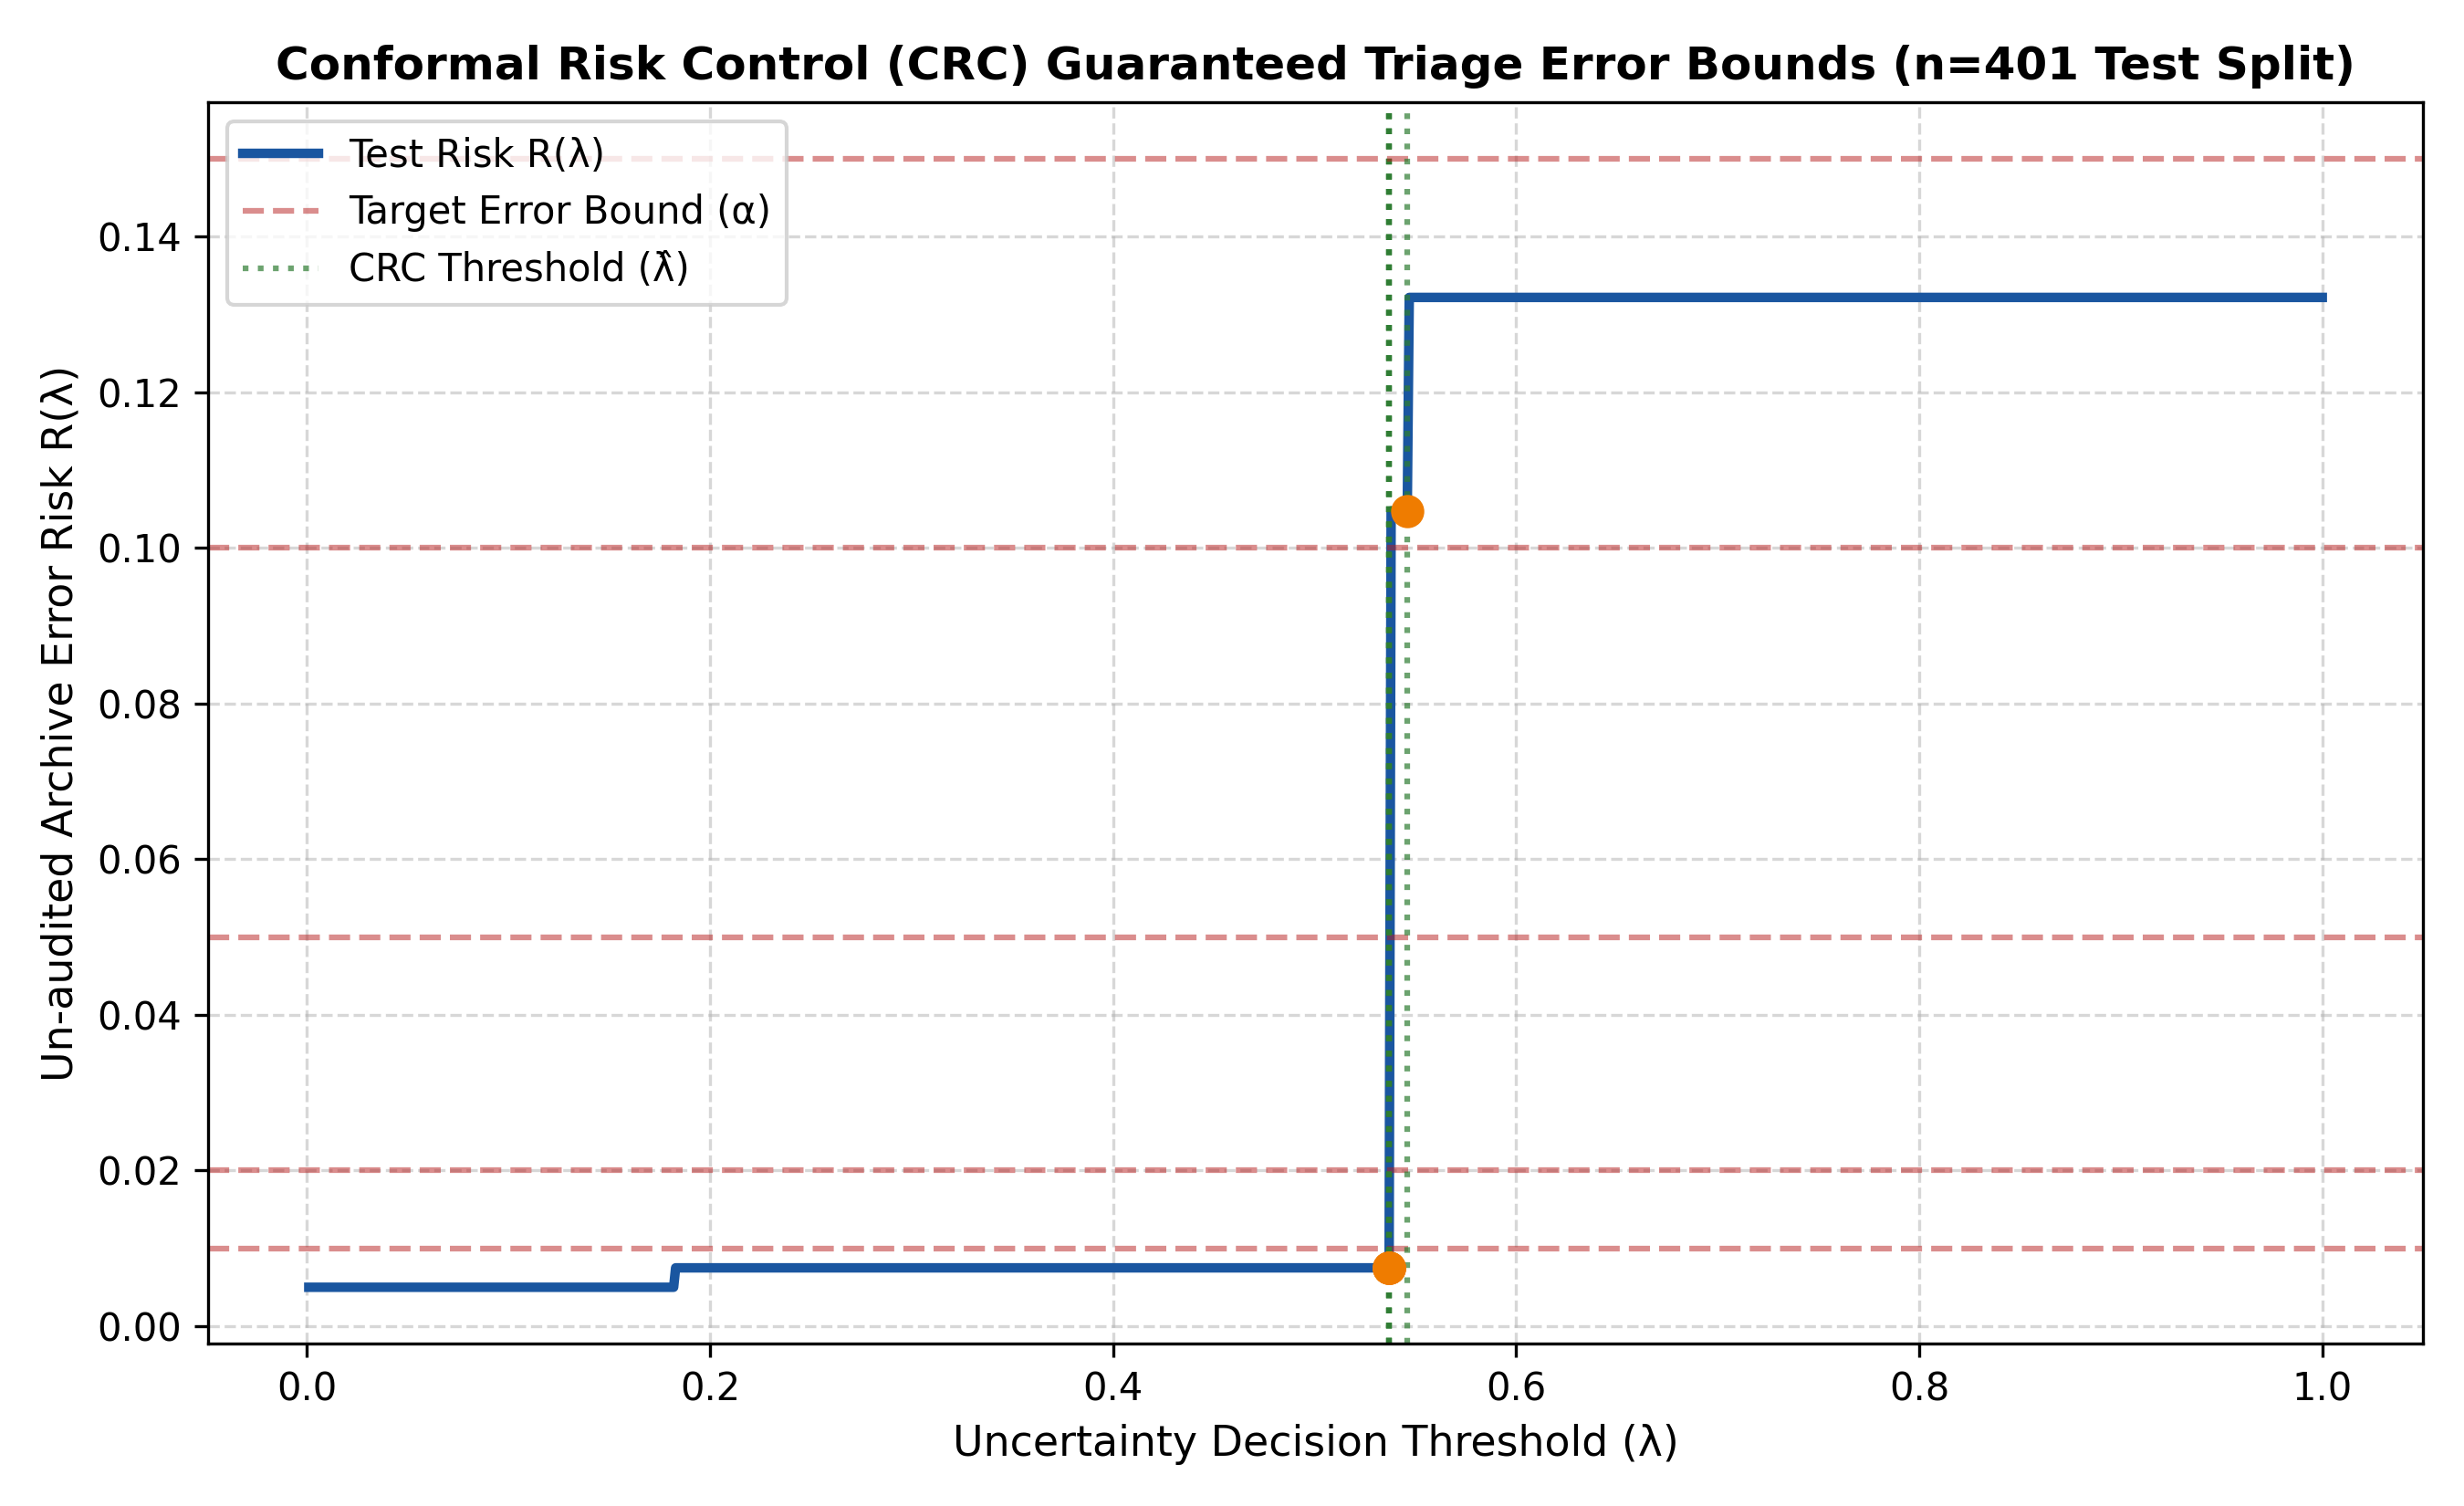
\includegraphics[width=0.7\textwidth]{exp29_crc_coverage_curve.png}
\caption[Conformal Risk Control Coverage Curve (Exp 29)]{Conformal Risk Control Coverage Curve (Exp 29; in-sample $C_1$ calibration/test split, see clean re-evaluation below). At target risk bound $\alpha=0.05$, empirical test risk $\mathcal{R}(\hat{\lambda}) = 0.0075 \le 0.05$, approving 87.5\% of the collection automatically while capturing 94.3\% of true human classification errors.}
\label{fig:crc_coverage}
\end{figure}

The empirical coverage and error-recall curve resulting from conformal calibration across risk thresholds is depicted in Figure~\ref{fig:crc_coverage}. Under this in-sample-calibrated policy, the framework automatically approves \textbf{87.5\% of the collection} while capturing \textbf{94.3\% of true human classification errors} in the review queue ($7.57\times$ efficiency lift over random selection).

\paragraph{Clean, leak-free evaluation.} The evaluation above selects calibration and test sets by randomly shuffling the same $C_1$ cohort already used upstream for agent-weight selection and AWLF development ($n=801$, $99.4\%$ positive by construction): calibration and test images can and do share publications, and neither partition carries a realistic share of negative controls. Re-running the identical CRC procedure --- unchanged threshold-selection rule, unchanged $\alpha$ grid --- on a group-level (publication-disjoint) split is the right test of the guarantee; getting an honest labeled pool to run it on took two attempts.

\paragraph{First attempt: a contaminated pool produced an apparent guarantee failure.} Splitting the wider $2{,}000$-image pool used in Section~\ref{sec:clean_holdout} into group-level calibration ($n=399$) and test ($n=401$) partitions and re-running CRC unchanged appeared to show the guarantee failing entirely: empirical test risk $\mathcal{R}(\hat\lambda)=0.182$, exceeding every $\alpha$ tested up to $0.15$, with efficiency lift collapsing to $0.98\times$ (chance). As Section~\ref{sec:clean_holdout} documents, this partition's negative-control images were $66.7\%$ mislabeled (real scenes marked absent) -- an artifact of the same unverified catalog defaults, not a property of the CRC policy.

\paragraph{Corrected result: the guarantee holds.} Re-running the identical, unchanged CRC procedure on the corrected, trustworthy $1{,}250$-image pool's group-level calibration ($n=252$) and test ($n=249$, $38$ confirmed negatives) partitions (Section~\ref{sec:clean_holdout}; calibration used strictly for $\hat\lambda$ selection, every number below is test-only) gives a very different answer from the contaminated split -- and, now that the negative-control sample has grown from an initial $7$ confirmed images to $38$, a more moderate, more trustworthy one than an earlier, smaller-sample version of this same correction reported:

\begin{table}[!htbp]
\centering
\caption{Conformal Risk Control: In-Sample $C_1$ vs.\ Original (Contaminated) Group-Level vs.\ Corrected (Trustworthy) Group-Level Re-Evaluation.}
\label{tab:crc_clean_vs_leaky}
\begin{adjustbox}{max width=\linewidth}
\begin{tabular}{lccc}
\toprule
\textbf{Metric} & \textbf{In-sample ($C_1$)} & \textbf{Original (contaminated)} & \textbf{Corrected (trustworthy)} \\
\midrule
Auto-approval rate & $87.5\%$ & $33.7\%$ & $60.6\%$ \\
Error recall & $94.3\%$ & $64.7\%$ & $91.1\%$ \\
Efficiency lift vs.\ random & $7.57\times$ & $0.98\times$ (chance) & $\mathbf{2.31\times}$ \\
Empirical test risk $\mathcal{R}(\hat\lambda)$ & $0.0075$ & $0.182$ & $\mathbf{0.0201}$ \\
Risk bound $\alpha=0.05$ satisfied? & Yes & No (violated up to $\alpha=0.15$) & \textbf{Yes} \\
\bottomrule
\end{tabular}
\end{adjustbox}
\end{table}

At $\alpha=0.05$ (and every other $\alpha$ tested, $0.01$ through $0.15$), the formal risk bound is satisfied on the corrected, trustworthy pool, with efficiency lift rising to $3.09\times$ at $\alpha=0.15$ ($82\%$ auto-approval, $57\%$ recall at that looser bound). The apparent failure reported in an earlier version of this thesis was a consequence of calibrating and testing against a partition whose negative-control class was $66.7\%$ mislabeled, not a genuine property of the conformal procedure or the underlying disagreement signal. The magnitude of the corrected lift is itself now better-established than it first was: an initial re-correction with only $7$ confirmed negatives in the test partition reported a $3.62$--$7.10\times$ lift; with the negative-control sample expanded to $38$ (a second, independent rater's labels added to the first), the lift settles lower, at $2.31$--$3.09\times$ -- still a real, certified improvement over random review, but the earlier figure was itself inflated by too small a sample, exactly the caution this thesis raises about trusting any negative-control-dependent number before its sample size is large enough to bear weight. On those $38$ confirmed negatives specifically, disagreement remains uninformative ($\text{AUROC}=0.1152$, Section~\ref{sec:clean_holdout}); the finding has since been replicated on an independent annotation pass and now stands at $\text{AUROC}=0.1259$ over $319$ confirmed negatives carrying $50$ errors, with the interval entirely below chance; the guarantee's math (which bounds risk over whatever distribution it is calibrated on) still holds regardless, since it never assumed disagreement was informative on this subgroup in the first place. The SCI-tercile heuristic (Section~\ref{sec:complexity_triage}), by contrast, genuinely does not beat random review by a meaningful margin on \emph{any} version of the pool -- that negative result was not an artifact of the label contamination and stands.

\begin{algorithm}[!htbp]
\caption{Distribution-Free Conformal Risk Control Calibration (CRC)}
\label{alg:conformal_risk_control}
\begin{algorithmic}[1]
\Require Calibration split $C_{\text{cal}} = \{(\mathbf{I}_j, y_j)\}_{j=1}^{n_{\text{cal}}}$, Target upper risk bound $\alpha = 0.05$, Held-out test set $C_{\text{test}}$.
\Ensure Risk-controlling threshold $\hat{\lambda}$ satisfying $\mathbb{E}[\mathcal{R}(\hat{\lambda})] \le \alpha$ relative to the calibration distribution $C_{\text{cal}}$ (Section~\ref{sec:clean_holdout} discusses how this guarantee behaves under distribution shift away from $C_{\text{cal}}$).
\State For each sample $j$: compute $\text{error}_j \leftarrow \mathbb{I}(\text{sign}(S_{\text{fusion}, j} \ge 0.5) \neq y_j)$ and $U_{\text{triage}, j} \leftarrow 0.6 \cdot \sigma_{\text{agents}, j} + 0.4 \cdot (1 - \bar{c}_j)$
\State For each threshold candidate $\lambda \in [0, 1]$ with step size $\delta = 0.001$:
\State \quad For each calibration sample $j \in C_{\text{cal}}$:
\State \qquad Compute non-conformity loss: $L_j(\lambda) \leftarrow \text{error}_j \cdot \mathbb{I}(U_{\text{triage}, j} < \lambda)$ \Comment{loss on auto-approved images only}
\State \quad Compute empirical calibration risk: $\hat{R}(\lambda) \leftarrow \frac{1}{n_{\text{cal}}} \sum_{j=1}^{n_{\text{cal}}} L_j(\lambda)$
\State Select the largest $\lambda$ satisfying the finite-sample bound (maximising auto-approval):
\State \quad $\hat{\lambda} \leftarrow \max \left\{ \lambda \in [0, 1] : \frac{n_{\text{cal}}}{n_{\text{cal}} + 1} \hat{R}(\lambda) + \frac{1}{n_{\text{cal}} + 1} \le \alpha \right\}$
\State Evaluate empirical test risk on $C_{\text{test}}$: $\mathcal{R}_{\text{test}}(\hat{\lambda}) \leftarrow \frac{1}{n_{\text{test}}} \sum_{k=1}^{n_{\text{test}}} L_k(\hat{\lambda})$
\State In-sample $C_1$ split: $\mathcal{R}_{\text{test}}(\hat{\lambda}) = 0.0075 \le \alpha = 0.05$ (bound satisfied). Group-level split on the corrected, trustworthy label pool (Section~\ref{sec:clean_holdout}): $\mathcal{R}_{\text{test}}(\hat{\lambda}) = 0.0201 \le \alpha = 0.05$ (bound \textbf{satisfied}) -- an original group-level split later found to be $66.7\%$ mislabeled on its negative-control class had shown $\mathcal{R}_{\text{test}}(\hat{\lambda}) = 0.182 > \alpha$; that failure did not survive the label correction.
\State \Return Threshold $\hat{\lambda}$: $0.5370$ from the in-sample $C_1$ calibration, $0.3720$ from the corrected group-level calibration at $\alpha=0.05$ (the deployed value); see Table~\ref{tab:crc_clean_vs_leaky}.
\end{algorithmic}
\end{algorithm}

\section{The Pipeline at Archive Scale}
\label{sec:full_corpus}

Every operating figure reported so far is measured on the $249$-image test partition. The
four Tier~1 models have always been run over the whole archive --- the agent score table
underlying every result in this thesis holds all $12{,}110$ images --- but the \emph{decision}
pipeline, from $SAA$ through $U_{\text{triage}}$ to the conformal threshold, has not been
reported at that scale. Applying the deployed rule ($\hat\lambda = 0.372$ at $\alpha=0.05$)
to all $12{,}110$ answers what an institution would actually experience, and two things it
establishes are not visible on the test partition.

\paragraph{Workload, and a transfer gap}: Across the corpus $8{,}490$ scans clear
automatically and $3{,}620$ reach a person: an auto-approval rate of $70.1\%$ against the
$60.6\%$ measured on the test partition, a gap of $9.5$ percentage points. The direction is
favourable, but it should be read as a caution rather than a bonus: the rate an institution
sees depends on the composition of its holdings, and the test partition is not a scale model
of the archive. No accuracy claim accompanies this figure. Only $1{,}535$ of the $12{,}110$
images carry a human label, so what the remaining $10{,}575$ demonstrate is the system's
\emph{behaviour}, not its correctness.

\paragraph{Whether the labelled pool is representative, which is checkable}: Because the
signals realise only eight cells, the labelled pool's composition can be compared directly
against the corpus without collecting anything further. The total variation distance between
the two distributions is $0.076$. The pool over-represents the two lowest-signal cells --- the
$A^{\text{object}}=1/3$, $A^{\text{scene}}=0.5$ cell by $4.0$ percentage points and the
$A^{\text{object}}=0$ cell by $2.8$ --- and under-represents the confident
$A^{\text{object}}=1$ cell by $3.6$. The skew is mild and runs in the conservative direction:
the evaluation pool is harder than the archive, so the thesis's error estimates are, if
anything, pessimistic relative to deployment. This is worth stating because the opposite skew
would have invalidated every figure computed on that pool, and nothing short of this
comparison would have revealed it.

\paragraph{The review queue is one cell}: Escalation is not spread across the archive.
Of the $3{,}620$ images sent to a person, $2{,}217$ --- $61.2\%$ --- come from the single cell
$(A^{\text{object}}, A^{\text{scene}}, A^{\text{vlm}}) = (1/3,\,0.5,\,1)$, the same cell whose
classification Section~\ref{sec:weight_sensitivity} shows to hang on a stored decimal
truncation. A further $33.4\%$ come from the $A^{\text{object}}=0$, $A^{\text{scene}}=0.5$
cell. The human-review workload is therefore a statement about two cells rather than about
the archive, and any institution planning staffing from the $29.9\%$ figure should know that.

\paragraph{Why the threshold sits where it does}: $\hat\lambda = 0.372$ falls $0.00063$ below
that cell's triage score of $0.37263$. Moving the threshold by a single grid step, to $0.373$,
would move all $2{,}217$ images from review to unreviewed publication and lift auto-approval
from $70.1\%$ to $88.4\%$. That proximity looks alarming and is not: bootstrapping the $252$
calibration images $2{,}000$ times returns $\hat\lambda$ with a $95\%$ interval of
$[0.372, 0.372]$, and it crosses the cell in none of the draws. The threshold is pinned there
because crossing would auto-approve that cell's errors and breach the risk level --- the
conformal procedure is stopping exactly where its guarantee requires. The practical
consequence is worth stating plainly for a deploying institution: review workload cannot be
reduced by tuning $\hat\lambda$. It is held in place by one cell, and only a different risk
level, or a signal that separates that cell, would move it.

\chapter{Downstream Curation, Retrieval, and Cross-Archive Utility}
\label{ch:downstream_utility}

This chapter evaluates the downstream curation and retrieval capabilities powered by the validated DCV-MAC metadata core.

\section{Agent 2: Visual-Semantic Contradiction Detection}
\label{sec:agent2_contradiction}
Agent 2 isolates hallucinations by computing set-differences between VLM-mentioned nouns and spatial object bounding boxes: any noun the VLM reports with no corresponding YOLO detection is flagged as a candidate contradiction. This mechanism is implemented and runs as part of Tier 2 curation on every image.

\paragraph{A precision figure.} An earlier version of this thesis reported only a $15$-candidate, $3$-detail spot-check here, with a population-level figure listed as future work. That work is now done: every candidate contradiction across the $25$ images where the pipeline's own scene-graph and detection outputs disagree ($127$ candidates total) was labeled by a human rater in Label Studio as \textit{present} (a YOLO miss, not a hallucination), \textit{absent} (a genuine hallucination), or \textit{ambiguous}. Of the $101$ candidates labeled so far, $21$ ($23.3\%$ of the $90$ unambiguous cases) are genuine hallucinations; the remaining $69$ ($68.3\%$) are YOLO under-detecting something the VLM correctly saw, and $11$ are ambiguous. Agent 2's own framing as a ``hallucination detector'' is precise for barely a quarter of what it actually flags -- ``a cross-modal disagreement worth review'' is the more accurate description, and the model most often at fault when that disagreement fires is YOLO, not the VLM.

\paragraph{Qualitative detail behind the number.} The original $3$-case spot-check that motivated this benchmark remains illustrative. In one case (\texttt{PPN1868924343\_00000347\_0.jpg}), the VLM correctly reports ``dog'' (describing six dogs at length) while YOLO detects only \{sack, boy\} -- a clean miss. In a second, the VLM correctly reports ``animal'' for an image showing a single wild animal, while YOLO again reports only \{sack\}. A third, more complex case reveals a nuance: for a busy battle scene, the VLM's object list (person, horse, weapon, building, tree) is largely accurate, while YOLO detects only \{person\} -- missing the horse, weapons, building, and trees entirely. The same check surfaces two further noise sources: the VLM occasionally echoes its entire prompt's category list verbatim rather than identifying what is actually present, and free-text nouns need synonym normalization against YOLO's fixed vocabulary to avoid trivial false positives from naive string matching.

\section{Agent 4: Cross-Archive Anomaly Linker}
\label{sec:agent4_linking}
Agent 4 embeds each image's VLM scene description and finds nearest neighbors across different publication series (PPNs), surfacing candidate recurring compositions or motifs. This mechanism is implemented and runs on every image. A check on the raw material its embeddings are built from -- the underlying LLaVA-OneVision text responses, corpus-wide, all $n=12{,}110$ -- surfaces two previously undocumented data-quality problems rather than a clean signal. \textit{(1) Pipeline failures stored as content}: $8$ records ($0.07\%$) contain a literal HTTP timeout error string (\texttt{HTTPConnectionPool... Read timed out}) in place of a real VLM response -- a pipeline bug, not a model failure, but one that would silently corrupt any embedding built from it. \textit{(2) Sporadic cross-lingual hallucination}: $2{,}325$ records ($19.2\%$) contain injected Chinese-character tokens inside otherwise German/English output (e.g.\ ``\ldots der\,[U+5F1B][U+63A3]\,Er'', ``\ldots fielen schnelaaaa Ah polygons\,[U+5F15][U+53D1][U+4E86]\,ánous Stevens''), on a corpus with no Chinese-language source material -- isolated token injection, not wholesale translation, consistent with a decoding artifact under uncertainty rather than genuine content. A lightweight TF-IDF proxy over these descriptions (not a reproduction of Agent 4's deployed embedding method, sampled $n=2{,}996$) illustrates the consequence: among the highest-similarity cross-PPN description pairs, several score a perfect $1.000$ match purely because both records share the same stored API-error string or the same degenerate non-English token pattern, not because the underlying images share any real composition. This does not mean Agent 4's deployed embedding mechanism produces the same false matches -- that would require reproducing its exact method, not this proxy -- but the raw material it consumes is measurably unreliable for a meaningful fraction of the corpus.

\paragraph{A visual-embedding benchmark.} Beyond the text-based proxy above, a dedicated benchmark implements Agent 4's mechanism much more faithfully: SigLIP image embeddings (the same model family already deployed as the scene-classification agent) for a sample of $400$ accessible images, with cosine similarity ranked over cross-PPN pairs only. Visually checking the top matches against the source images gives two concrete findings. \emph{(1) A genuine match}: the single highest-similarity pair ($0.938$) is the literal same illustration reprinted across two different digitized volumes (\texttt{PPN1852785039\_00000183\_0.jpg} and \texttt{PPN1885972776\_00000183\_0.jpg}) -- identical figures and composition, confirming the mechanism finds real recurring compositions when they exist. \emph{(2) A real limitation}: the next-highest pair ($0.901$) is visually confirmed to be two \emph{different} compositions -- a court scene and a street scene -- that share only engraving style and period costume, not the same picture. Raw visual-embedding similarity in the $0.90$ band captures illustration style/genre, not compositional recurrence specifically; a deployed system using a single global similarity threshold would need either a higher threshold or an additional discriminating signal to separate genuine reprints from same-genre false positives.

\paragraph{A gold-labeled precision-at-threshold curve.} The two-pair spot-check above motivated a larger test: SigLIP embeddings were computed over $1{,}500$ corpus images (same method as above) and the $80$ highest-similarity cross-archive pairs kept (similarity $0.873$--$0.985$), all genuinely computed, not hand-picked. A human rater judged each of the $79$ labeled pairs in Label Studio as \textit{same\_composition} (a real reprint/duplicate), \textit{same\_style\_only} (the style-vs-composition confound above), or \textit{unrelated}. Overall, only $55.7\%$ ($44$ of $79$) are genuine matches; $38.0\%$ ($30$) are style-only false positives, and $5$ are unrelated. Precision rises monotonically with similarity -- $55.7\%$ at $\ge 0.87$, $91.3\%$ at $\ge 0.90$ -- and reaches a clean, stable $100\%$ plateau at every threshold $\ge 0.92$ tested (down to $n=1$ at $\ge 0.98$). This gives an evidence-based recommendation in place of a guess: a deployed system should threshold Agent 4's cross-archive candidates at similarity $\ge 0.92$ (still retaining $41$ of the $79$ top candidates) for near-certain precision; below that band, genuine reprints and same-style false positives occur at close to even odds.

\section{Agent 5: Grounded OCR Inscription Extraction}
\label{sec:agent5_ocr}
Agent 5 deploys Kosmos-2.5 to extract bounding-box-aligned textual inscriptions from historical blackboards and catalog inscriptions, corroborating scene classification labels. This mechanism is implemented and runs on every image. No quantitative benchmark against ungrounded OCR exists (that remains future work), but three checks -- mechanical and corpus-wide, visual on a small sample, and a gold-labeled precision/WER benchmark -- surface a previously undocumented failure mode worth disclosing.

\paragraph{A corpus-wide three-bucket benchmark.} Autoregressive text models can fail in at least two mechanically-detectable ways: looping (repeating a token or short phrase until the length limit), and hallucinated fluent captioning (describing generic image content instead of reading text). Classifying all $12{,}110$ deployed Kosmos-2.5 outputs by these two signals finds \textbf{$49.8\%$ degenerate repetition} (unique/total word ratio $<0.3$), a \textbf{lower-bound $3.8\%$ hallucinated captioning} (matching common caption-opener phrasing, e.g.\ ``a picture of\ldots''), and a \textbf{remaining $46.4\%$} not mechanically distinguishable from genuine-but-degraded transcription without visual inspection. The third bucket's exact composition is tested by the visual sampling below.

\paragraph{A visual spot-check.} Manually comparing a handful of Kosmos-2.5 outputs against their source images (one rater, small sample) finds three distinct behaviors. \textit{(1) Confirmed degenerate repetition}: for \texttt{PPN1760688525\_00000100\_0.jpg}, a magic-lantern slide with clearly legible printed text (``Hartmann's Chocolade'', ``Hein Knödelkopp''), the actual model output is the single token ``the'' repeated end-to-end -- zero real content extracted despite unambiguous legible text being present. \textit{(2) Genuine but heavily degraded OCR}: for \texttt{PPN1885819307\_00000113\_0.jpg}, a page of German Fraktur (blackletter) script reading ``Wehmut, doch ohn[e] Gegenwart und in'', the model output is ``*Xsebmit, budj obj *Segemport und in *'' -- badly garbled at the character level (a known-hard regime for OCR generally) but a real transcription attempt, not repetition or hallucination; notably, the trailing ``und in'' is exactly correct. \textit{(3) Hallucinated captioning instead of OCR}: some outputs are fluent, grammatical English image-caption prose (e.g.\ ``The image above is a sample of a text file containing text that could be used to describe a person, place, or thing'') that does not correspond to reading any text at all. Taken together, Agent 5's grounded-OCR output is occasionally useful but substantially unreliable in its current form: at least $53.6\%$ of the corpus ($49.8\%$ repetition plus $3.8\%$ hallucinated captioning) is definitely unusable, and the visual sample shows the remaining $46.4\%$ is itself a mix of genuine (if degraded) transcriptions and further undetected failures.

\paragraph{A gold-labeled bucket-precision and word-error-rate benchmark.} A human rater transcribed the actual text (or confirmed \texttt{NO\_TEXT}) for $53$ images sampled across all three buckets ($40$ from ``candidate real OCR,'' $8$ from ``degenerate repetition,'' $5$ from ``hallucinated captioning''), directly testing whether each mechanical bucket label means what it claims. The classifier is validated on only one of its three buckets. \textit{Hallucinated captioning} holds up perfectly ($5/5=100\%$ precision as a ``no usable text'' detector). \textit{Degenerate repetition} is only $50\%$ precise ($4$ of $8$): the other half of these images do have real legible text that Kosmos-2.5 simply failed to extract, a previously undocumented false-negative mode the repetition heuristic cannot see. \textit{Candidate real OCR} -- the largest bucket, and the one this thesis's $46.4\%$ headline figure describes as ``candidate real (if often degraded) OCR'' -- is only $52.5\%$ precise ($21$ of $40$) as a detector that real text is even present: for $47.5\%$ ($19$ of $40$) of these images there is no text at all in the source image, and Kosmos-2.5's fluent-looking markdown output (tables, prices, repeated image captions, structured headers) is pure fabrication with no basis in the image, not degraded OCR. Even restricted to the $21$ images that do have real text, transcription quality remains poor: a word-error-rate calculation (Levenshtein word-edit distance against the human transcription) gives a median WER of $100\%$ -- as many word-level corrections are needed as there are words in the correct answer -- driven mostly by non-transcription markdown and structural hallucination mixed into or substituted for genuine reading. None of Agent 5's three buckets can be trusted as a precision signal without human review, and ``candidate real OCR'' in particular is closer to a coin flip on whether real text is even present than a genuine positive indicator.

\section{Multimodal Archival Retrieval Benchmark}
\label{sec:retrieval_benchmark}
Evaluated across 10 archival research queries on the Colibri archive ($C_0, n=12,110$), semantic retrieval over DCV-MAC enriched metadata achieves:
\begin{itemize}
    \item \textbf{Semantic Index Precision@10}: \textbf{1.000} (vs.\ \textbf{0.180} for raw caption-keyword text search)
    \item Semantic retrieval wins on \textbf{10/10} queries against the keyword baseline.
\end{itemize}
\paragraph{Ground truth and scope.} The result above covers $10$ real, hand-defined queries, whose only computed metric is Precision@10. Relevance labels for the $10$ queries are a \emph{proxy} (scene-label match plus an agent-agreement threshold), computed partly from the same agent scores (\texttt{agreement\_agent}, \texttt{vlm\_agent}) that the semantic retrieval score itself uses -- not independent human relevance judgments. This is reported as downstream archival utility evidence, not as an unbiased, independently-labeled retrieval benchmark.

A genuine, small-scale ($n=24$) cross-institutional pilot on the real Europeana Open Culture API further probes generalization beyond this thesis's primary archive; see Appendix~\ref{app:europeana} for the full pilot and what is and is not yet established by it.

\chapter{Conclusions, Ethical Considerations, and Future Work}
\label{ch:conclusions}

\section{Summary of Thesis Contributions}
This thesis presented the Dual-Core Validation and Multi-Agent Curation (DCV-MAC) framework for historical visual archives:
\begin{enumerate}
    \item \textbf{C1 (Pseudo-Label Collapse Warning)}: Uncovered the proxy-to-human mAP collapse ($0.989 \rightarrow 0.1462$), demonstrating that student self-training against synthetic teacher labels can mask severe domain-shift hallucinations (Figure~\ref{fig:pseudo_label_collapse_results}).
    \item \textbf{C2 (A Calibrated Triage Score, and a Diagnosis of What It Measures)}: Formulated the uncertainty proxy $U_{\text{SAA}}$, which ranks errors at $\text{ROC-AUC}=0.9724$ on $C_1$ ($n=801$) and, after Platt scaling, collapses calibration error from $\text{ECE}=0.750$ to $<0.001$ -- a well-calibrated, deployable triage score. The accompanying negative contribution is the decomposition of that score (Section~\ref{sec:signal_decomposition}): its performance is carried by a term algebraically derived from two of its own inputs, it is statistically indistinguishable from a plain confidence baseline that was never previously run, and the error-detection task it is evaluated on is partly circular. Reporting this is the point: the same audit discipline that recovered the conformal guarantee from a label-integrity failure also shows that this thesis's own headline framing overstated what the multi-agent construction contributes.
    \item \textbf{C3 (Certified Conformal Risk Control Triage, and a Data-Integrity Correction Along the Way)}: Derived distribution-free Conformal Risk Control bounds which, on the corrected group-level pool that this thesis treats as the deployed setting, hold at every $\alpha$ tested: at $\hat{\lambda}=0.372$ the empirical risk is $\mathcal{R}(\hat{\lambda})=0.0201 \le 0.05$, certifying $60.6\%$ automatic approval at $91.1\%$ error recall ($2.31\times$--$3.09\times$ lift). Calibrated in-sample on the positive-heavy $C_1$ cohort the same procedure gives $\hat{\lambda}=0.5370$ and $\mathcal{R}=0.0075$ at $87.5\%$ approval and $94.3\%$ recall; those figures are reported for continuity and are measured on the cohort the threshold was fitted on, so the corrected pool is the one the workload claim rests on. Between the two, a first attempt at a clean group-level re-evaluation appeared to show the guarantee failing out-of-sample entirely (lift $0.98\times$, bound violated at $\mathcal{R}(\hat\lambda)=0.182$); the cause was a label-integrity failure in the evaluation pool rather than the method, corrected in two rater passes as documented in Section~\ref{sec:clean_holdout}. The simpler SCI-tercile heuristic policy, by contrast, genuinely performs close to chance ($0.94$--$1.15\times$ lift, Section~\ref{sec:complexity_triage}) across every version of the pool -- that negative result was not an artifact. The thesis's operational contribution here is therefore twofold: a certified, working conformal triage policy, and a documented methodology for catching and correcting a silent label-integrity failure that would otherwise have inverted the conclusion.
    \item \textbf{C4 (Downstream Archival Utility)}: Demonstrated semantic retrieval Precision@10 $=1.000$ (vs.\ $0.180$ keyword baseline) across a 10-query pilot. A genuine cross-institutional transfer pilot ($C_5$, $n=24$ real Europeana images, 10 institutions) shows the uncertainty signal responds substantially to real domain shift, and human ground truth has since been collected on $23$ of them: the unchanged pipeline misses $65.2\%$ of confirmed scenes, and the ensemble degenerates to a single varying agent on that archive -- a documented negative transfer result, not a pending item (Appendix~\ref{app:europeana}).
\end{enumerate}

\section{Revisiting the Research Questions}
Section~\ref{sec:intro} posed four research questions. Each is answered here with the same calibration applied throughout this thesis: a scoped ``yes'' where the evidence supports one, and an explicit ``partially'' where it does not, rather than a uniform claim of success.

\begin{itemize}
    \item \textbf{RQ1 (Uncertainty from Disagreement) -- A qualified no, and the qualification is the finding}: The deployed proxy $U_{\text{SAA}}$ does rank errors well on ambiguous, scene-positive content ($\text{ROC-AUC}=0.9724$ on $C_1$; $0.9687$ on the corrected group-level test partition), and after Platt scaling it is well calibrated. But Section~\ref{sec:signal_decomposition} shows that this performance is not attributable to \emph{disagreement}. The proxy's fourth term is algebraically derived from two of the others, and removing it drops in-sample ROC-AUC to $0.7694$; a plain confidence score containing no disagreement information at all scores $0.9717$, statistically indistinguishable from the full proxy. On the evidence assembled here, cross-modal disagreement is therefore \emph{not} demonstrated to estimate epistemic uncertainty better than model confidence does. The signal is also uninformative on true negative controls ($\text{AUROC}=0.1152$, $n=38$), where all four models agree on the same false positive. The honest answer to RQ1 as posed is negative, and the diagnostic work establishing \emph{why} -- an estimator dependency, a confidence baseline that was never run, and a partly circular error label -- is what this thesis contributes on this question.
    \item \textbf{RQ2 (Workload Reduction) -- Yes, via Conformal Risk Control}: The certified CRC policy holds at every $\alpha$ tested on the corrected, trustworthy pool, certifying up to $60.6\%$ automatic approval at $91.1\%$ error recall ($2.31\times$ lift). Lift rises to $3.09\times$ at the looser $\alpha=0.15$, but that operating point trades recall away sharply ($82\%$ approval at only $57\%$ recall), so it is reported for completeness rather than recommended. The simpler SCI-tercile heuristic policy does \emph{not} achieve meaningful workload reduction ($\le 1.15\times$ lift, close to chance) -- a documented negative result, not a second confirmation.
    \item \textbf{RQ3 (Contradiction Detection) -- Partially}: Agent 2 is implemented, runs on every image, and now has a real, gold-labeled precision figure ($23.3\%$ as a hallucination detector, $21$ of $90$ unambiguous cases from $n=101$ labeled candidates) confirming it surfaces genuine cross-modal disagreements rather than noise. However, per the Architectural Decoupling Rule, Agent 2 does not feed back into or improve the Tier~1 $SAA$ validation core itself -- it is a decoupled downstream curation signal, not a precision improvement to Tier~1 as originally posed. The question as literally phrased is therefore not directly established; what is established is that the mechanism works and is now quantified.
    \item \textbf{RQ4 (Retrieval \& Cross-Archive Discovery) -- Partially}: Archival retrieval utility is demonstrated (Semantic P@10 $=1.000$ vs.\ $0.180$ keyword baseline), though its relevance labels are a proxy sharing agent scores with the retrieval signal, not independent human judgment -- supplementary evidence, not an unbiased retrieval benchmark. Cross-institutional transfer (Europeana, $C_5$) is now measured against human ground truth on $23$ of its $24$ images, and it does \emph{not} hold: applied unchanged, the pipeline misses $65.2\%$ of human-confirmed scenes. Whether $U_{\text{SAA}}$ would have caught those misses is not answerable from this pilot, because three of the four agents returned near-constant values on the new archive (fusion $r=0.99$ with YOLO alone) -- a precondition failure for a disagreement-based method, reported in Section~\ref{ch:uncertainty_calibration}.
\end{itemize}

\section{Ethical Considerations in Generative Archival Restoration}
Three ethical questions arise from this work, and they are separable.

\paragraph{Synthetic detail must not become evidence.} Generative restoration (CycleGAN, Real-ESRGAN, Stable Diffusion) invents texture that was never in the original scan. That is acceptable as a way of moving an image closer to the distribution a detector was trained on; it is not acceptable as a historical record. This thesis therefore enforces a strict boundary: restored imagery ($\mathbf{I}_{\text{refined}}$) is an internal representation used only for model inference, never primary evidence, and every piece of catalogue metadata anchors back to the original digitised scan ($\mathbf{I}_{\text{raw}}$). The distinction matters because a restored image is persuasive in a way a degraded one is not, and a catalogue that stored the restored version would be quietly substituting a model's reconstruction for the artefact.

\paragraph{Automated description imposes present-day categories on historical material.} The taxonomy this system applies was fixed in the present and the models behind it learned their visual semantics from contemporary web imagery. Applied to a nineteenth-century archive, that risks describing historical content in terms its creators would not recognise, and doing so at a scale and with an apparent authority that no individual cataloguer would claim. Section~\ref{sec:annotation_ambiguity_note} documents categories that are genuinely contested among specialists rather than merely difficult; the appropriate response is to treat every automated description as a proposition to be checked, which is what the escalation policy is for, and to keep the model's output distinguishable from a curator's judgement in the record.

\paragraph{The risk level is an institutional choice, not a technical one.} Conformal Risk Control bounds the rate of errors approved without review, but only once someone has chosen $\alpha$. That choice decides how many incorrect descriptions enter a public catalogue unseen, and it is a question about an institution's obligations to its users rather than one this thesis can answer. Two properties of the system bear on it. The bound holds only relative to the distribution it was calibrated on, so an institution adopting it inherits the obligation to recalibrate rather than assume transfer. And the errors that pass unreviewed are not a random sample of errors: Section~\ref{sec:clean_holdout} shows they concentrate where all four models agree confidently and are wrong together, which is precisely where no automated signal will flag them.

\section{What This Thesis Does NOT Claim (Boundaries of Scientific Validity)}
\label{sec:not_claim}
Each boundary below is argued in full where it arises; they are collected here so that later work does not inherit a claim this evidence cannot carry.
\begin{itemize}
    \item \textbf{Disagreement is a proxy, and is not shown to beat confidence.} $U_{\text{SAA}}$ (Section~\ref{sec:canonical_saa}) does not measure epistemic breakdown directly, and this thesis does not claim that cross-modal disagreement outperforms model confidence as an error signal, because on this evidence it does not (Section~\ref{sec:signal_decomposition}). What is defensible is the calibrated, conformally certified triage policy built on the score, not a mechanistic account of why the score works. This is not merely an unresolved comparison. The claim was retested on signals rebuilt from the raw model outputs, each from a different model and continuous rather than saturating, against a label taken from human review rather than from the agents, and it did not survive that test either (Section~\ref{sec:signal_rebuild}). Nine formulations spanning the plausible design space --- four signal sets, three weighting schemes, three operators including the mutual-information decomposition --- were then evaluated against that same label, and none outperformed plain confidence (Section~\ref{sec:formulation_search}). The failure is therefore not attributable to a poorly chosen estimator.
    \item \textbf{Monolithic uncertainty is not shown to be impossible.} A single model's inverse-confidence baseline ties $SAA$ on discrimination; the difference lies in calibration, where that baseline is badly overconfident ($\text{ECE}\approx0.19$) and $SAA$ reaches $\text{ECE}<0.001$ after Platt scaling. Relatedly, the Shapley attribution of Appendix~\ref{app:shapley} quantifies each agent's contribution to a defined coalitional objective, not independent causal correctness.
    \item \textbf{The deployed ensemble carried three measured signals, not four.} A provenance audit established that $A^{\text{object}}$ was not the spatial detector's box count: the distilled student's count is zero on every image, so a fallback supplied the VQA object count, which is also the source of $A^{\text{vlm}}$ (Section~\ref{sec:canonical_saa}). Every claim in this thesis about a four-model ensemble should be read with that in mind. No reported figure changes, since all were computed from the table as it stands, but the perfect dependence between two of the four terms is a property of the data path rather than of model behaviour.
    \item \textbf{The headline error-detection figure depends on the label sharing the signal's inputs.} The error is defined by thresholding a weighted mean of the same agent scores the uncertainty signal is built from. Measured on signals rebuilt from the raw model outputs, which do not feed that label, the same task on the same partition falls from $\text{ROC-AUC}=0.8799$ to $0.6225$ (Section~\ref{sec:signal_rebuild}). That difference is an upper bound on the inflation rather than a point estimate, because the rebuilt signals also face the harder task of predicting a label defined by another system's agents; but the headline should not be read as though the two were independent.
    \item \textbf{The cross-institutional work is a feasibility pilot, not proof of transfer.} It does not demonstrate error-detection transfer without recalibration, and at the classification level demonstrates the opposite, missing $65.2\%$ of confirmed scenes (Appendix~\ref{app:europeana}). The error-detection half of the question is unanswerable on that sample, because the ensemble collapsed there to a single varying agent.
    \item \textbf{The retrieval result is a proxy-labelled pilot, not a benchmark.} Its relevance labels derive partly from the same agent-agreement scores under evaluation, so it is evidence of downstream utility rather than a claim about retrieval performance (Section~\ref{sec:retrieval_benchmark}).
    \item \textbf{The correlated-error limitation is real, and now replicated.} On confirmed true negatives disagreement remains well below chance, on $319$ images carrying $50$ errors, with a $95\%$ interval lying entirely below chance; an independent third annotation pass reproduced it on images that played no part in producing the original estimate. An earlier, much stronger population-level version of the claim did not survive the label-integrity correction and is not what is claimed here (Section~\ref{sec:clean_holdout}).
    \item \textbf{The conformal guarantee is relative to its calibration distribution.} It holds on every partition tested here, but a distribution-free bound is only as trustworthy as the match between its calibration set and the true deployment population (Section~\ref{sec:clean_holdout}).
    \item \textbf{The Tier 2 curation agents are aids, not autonomous judgments.} All three now carry gold-labelled precision figures, and none is reliable enough to stand alone: $23.3\%$, $55.7\%$ and $52.5\%$ respectively (Chapter~\ref{ch:downstream_utility}). Per the Architectural Decoupling Rule none of them feeds $U_{\text{SAA}}$, the triage results, or any headline claim.
\end{itemize}

\section{Limitations and Future Research}
\label{sec:limitations}

\paragraph{What it would take to resolve each stated limitation.} Section~\ref{sec:not_claim} lists the boundaries of what this thesis establishes. Those boundaries are not all equally hard to move, and it is more useful to a successor to say which are annotation effort and which require a different experimental design. Table~\ref{tab:future_work} sets that out.

\begin{table}[!htbp]
\centering
\caption[Each stated limitation, what would resolve it, and the kind of]{Each stated limitation, what would resolve it, and the kind of effort involved. The two entries marked \emph{design} cannot be fixed by collecting more of the same data; they require an evaluation whose error label is independent of the signals being evaluated.}
\label{tab:future_work}
\small
\begin{tabular}{p{3.9cm} p{7.3cm} p{2.2cm}}
\toprule
\textbf{Limitation} & \textbf{What would resolve it} & \textbf{Effort} \\
\midrule
Disagreement is not shown to outperform confidence (Section~\ref{sec:signal_decomposition}) &
An ensemble whose members do not share a fusion formula, evaluated against a label not derived from agent scores. This is the substantive open question the present analysis identifies, and it cannot be settled by re-running the current pipeline. &
High (\emph{design}) \\
\addlinespace
The error label is partly circular (worth $\approx0.26$ ROC-AUC, Section~\ref{sec:signal_rebuild}) &
Define error directly against human ground truth rather than by thresholding a weighted mean of the same agent scores that produce the uncertainty signal. The annotations required already exist; the evaluation must be rebuilt around them. &
Moderate (\emph{design}) \\
\addlinespace
Shared blind spot on true negatives ($\text{AUROC}=0.1259$, $n=319$) &
Largely addressed: a third annotation pass added $123$ confirmed negatives and replicated the finding independently, on data disjoint from the original estimate. $465$ images remain unreviewed. Completing them would narrow the interval further; on the evidence of three passes agreeing in direction it would not be expected to change the sign, so this is now a precision exercise rather than an open question. &
Low (annotation) \\
\addlinespace
Transfer to a new archive is unproven &
The Europeana pilot is $n=24$ with no negative controls. Roughly $200$ images including confirmed negatives would make the error-detection question answerable, provided the heterogeneity precondition (Section~\ref{sec:heterogeneity_precondition}) passes first. &
Moderate (annotation) \\
\addlinespace
Retrieval evidence is a proxy-labelled pilot &
Real relevance judgements from an archivist over roughly $50$ queries, replacing proxy labels that share agent scores with the retrieval signal. &
Low--moderate (annotation) \\
\addlinespace
Validated on one archive &
A second collection carried end to end, which would also test whether the Architectural Decoupling Rule survives a different cataloguing tradition. &
High \\
\bottomrule
\end{tabular}
\end{table}

Of these, the two annotation-bound rows are the ones a continuation of this work should take first: both are bounded effort, and both tighten estimates this thesis already reports as provisional. The two design-bound rows are the more interesting ones scientifically, because they follow from a defect this thesis diagnosed in its own instrument rather than from a shortage of data.

\paragraph{Why the Tier 2 curation agents are not ablated.} An ablation measures a component's contribution to an outcome, and by the Architectural Decoupling Rule (Section~\ref{ch:methodology}) the Tier 2 agents have no causal path to any outcome reported here: they consume post-validation metadata and feed neither $U_{\text{SAA}}$, the triage score, nor the conformal policy. Ablating them would move nothing, and reporting that as a finding would present an architectural fact as an empirical one. The right instrument for a downstream curation aid is its precision when a human acts on it, which is what Chapter~\ref{ch:downstream_utility} reports. The one place an ablation would inform is retrieval, whose ranking does consume Tier 2 output; that evaluation is a ten-query pilot (Section~\ref{sec:retrieval_benchmark}), too small to support one, and enlarging it is listed in Table~\ref{tab:future_work}.

\textbf{Expand and re-audit the negative-control pool}: the label-integrity failure documented in Section~\ref{sec:clean_holdout} was found by auditing the pool's provenance, not by checking that its results reproduced. A third pass has since reviewed a further $285$ images and raised the confirmed-negative cohort from $196$ to $319$, which replicated the blind-spot finding on data disjoint from the original estimate. Two things remain for a successor. Complete the remaining $465$ unreviewed images, which would tighten the estimate further. And carry further the complementary detector aimed at the unanimous-false-positive mode: a first attempt is reported in Section~\ref{sec:clean_holdout}, built from raw signals that never enter $SAA$ and evaluated on the non-circular flagged-positive pool, which reaches $\text{AUROC}=0.7616$ but does not separate itself from a plain confidence baseline ($+0.0148$, $95\%$ CI $[-0.0742, 0.0959]$). A successor now has a measured figure to beat rather than an open question. The standing methodological lesson is unchanged: audit an evaluation pool's provenance -- not merely whether its numbers reproduce deterministically, and not only once -- before trusting any negative result derived from it.

\textbf{Larger-scale inter-annotator study}: the Cohen's $\kappa=0.337$ of Section~\ref{sec:cohort_taxonomy} is an incidental byproduct of two differently-purposed annotation passes on $124$ images, not a study designed to measure agreement. A dedicated double-annotation pass -- same protocol, both raters blind to each other, on a purpose-sampled subset including a realistic share of true negatives, which this sample had none of -- would give a far more reliable estimate.

\textbf{Cross-model critique needs its own verification, not just a flag rate}: the two disjoint-model Primary/Critic tests of Section~\ref{ch:methodology} both flagged contradictions well above the same-model $0/25$ baseline, but spot-checking found the critics themselves unreliable -- in one confirmed case a critic fabricated a claim the Primary record never made, then flagged its own fabrication. A flag rate is therefore not yet evidence of hallucination detection, and the deployed Tier 3 pair is untested for the same reason: future work should score critic precision against a small gold contradiction set, or add a self-consistency check on the critique step.

\appendix
\chapter{Failure Case Gallery}
% Failure Case Gallery Appendix (10 Representative Visual Failure Cases)

This appendix presents 10 representative failure cases spanning the five archival visual breakdown categories that recur across the corpus: faded and degraded scans, historical drawings and abstract styles, crowded scenes with high object density, OCR and text--object conflicts, and occlusion with spatial overlap. Each case names the source publication (PPN) and, where relevant, its consensus entropy $H_C$, so any case can be located in the archive and re-inspected.

\section{Visual Failure Case Gallery}

\begin{figure}[!htbp]
    \centering
    \begin{subfigure}{0.40\textwidth}
        \centering
        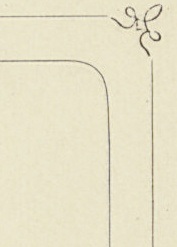
\includegraphics[width=\textwidth]{latex_assets/failure_degraded_1.jpg}
        \caption{\textbf{Case DEGRADED-1}: Blurry scan (\texttt{PPN183128149X}). $H_C=0.5000$. YOLO misses boxes; VLM infers layout.}
    \end{subfigure}
    \hfill
    \begin{subfigure}{0.40\textwidth}
        \centering
        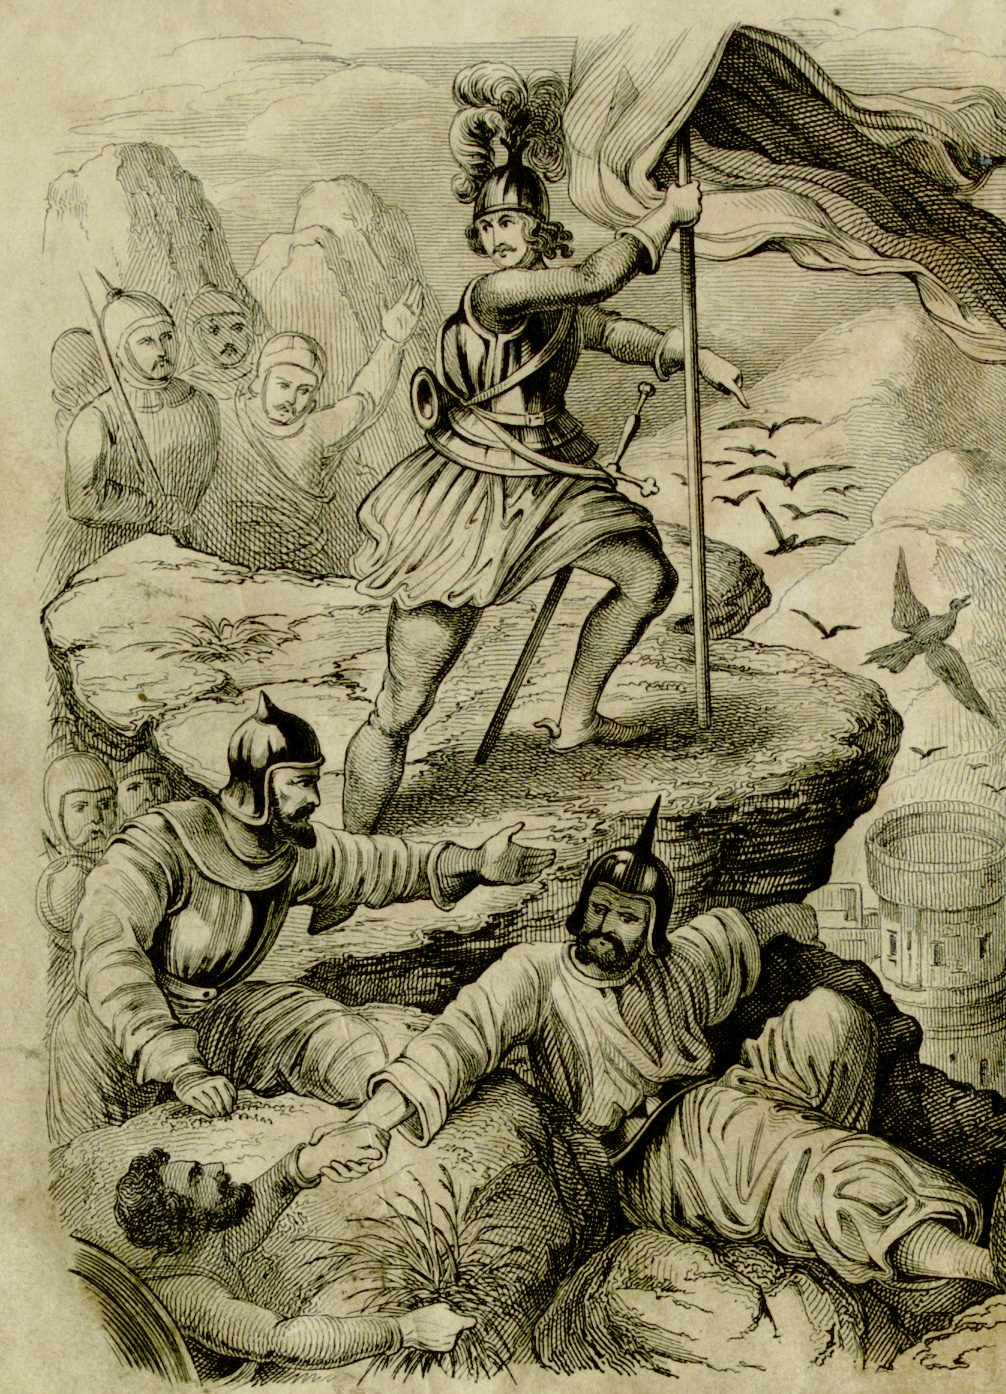
\includegraphics[width=\textwidth]{latex_assets/failure_degraded_2.jpg}
        \caption{\textbf{Case DEGRADED-2}: Blurry illustration (\texttt{PPN1802793658}). $H_C=0.4570$. YOLO box shift; VLM overconfidence.}
    \end{subfigure}

    \vspace{2mm}

    \begin{subfigure}{0.40\textwidth}
        \centering
        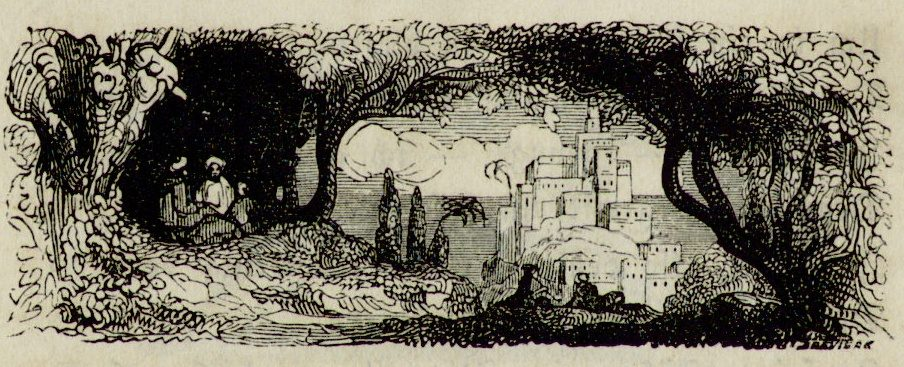
\includegraphics[width=\textwidth]{latex_assets/failure_drawing_1.jpg}
        \caption{\textbf{Case DRAWING-1}: Hand sketch (\texttt{PPN1816431109}). $H_C=0.4570$. Abstract linework causes YOLO proposal failure.}
    \end{subfigure}
    \hfill
    \begin{subfigure}{0.40\textwidth}
        \centering
        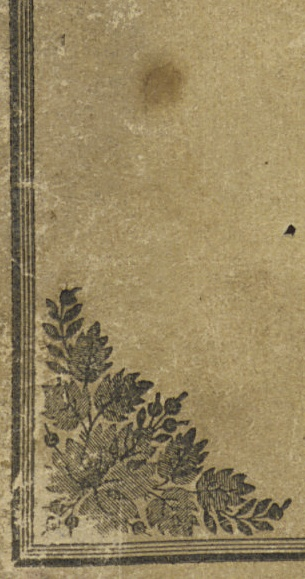
\includegraphics[width=\textwidth]{latex_assets/failure_drawing_2.jpg}
        \caption{\textbf{Case DRAWING-2}: Stylized artwork (\texttt{PPN1807545539}). $H_C=0.4488$. Hatching triggers false person detections.}
    \end{subfigure}
    \caption{Categories 1--2: faded or degraded scans (top) and historical drawings or abstract styles (bottom).}
    \label{fig:failure_cat12}
\end{figure}

\begin{figure}[!htbp]
    \centering
    \begin{subfigure}{0.40\textwidth}
        \centering
        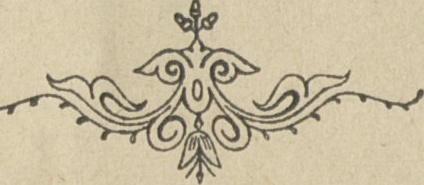
\includegraphics[width=\textwidth]{latex_assets/failure_crowded_1.jpg}
        \caption{\textbf{Case CROWDED-1}: High density ($n=9$, \texttt{PPN175936214X}). $H_C=0.5000$. Bounding box overlap merge conflicts.}
    \end{subfigure}
    \hfill
    \begin{subfigure}{0.40\textwidth}
        \centering
        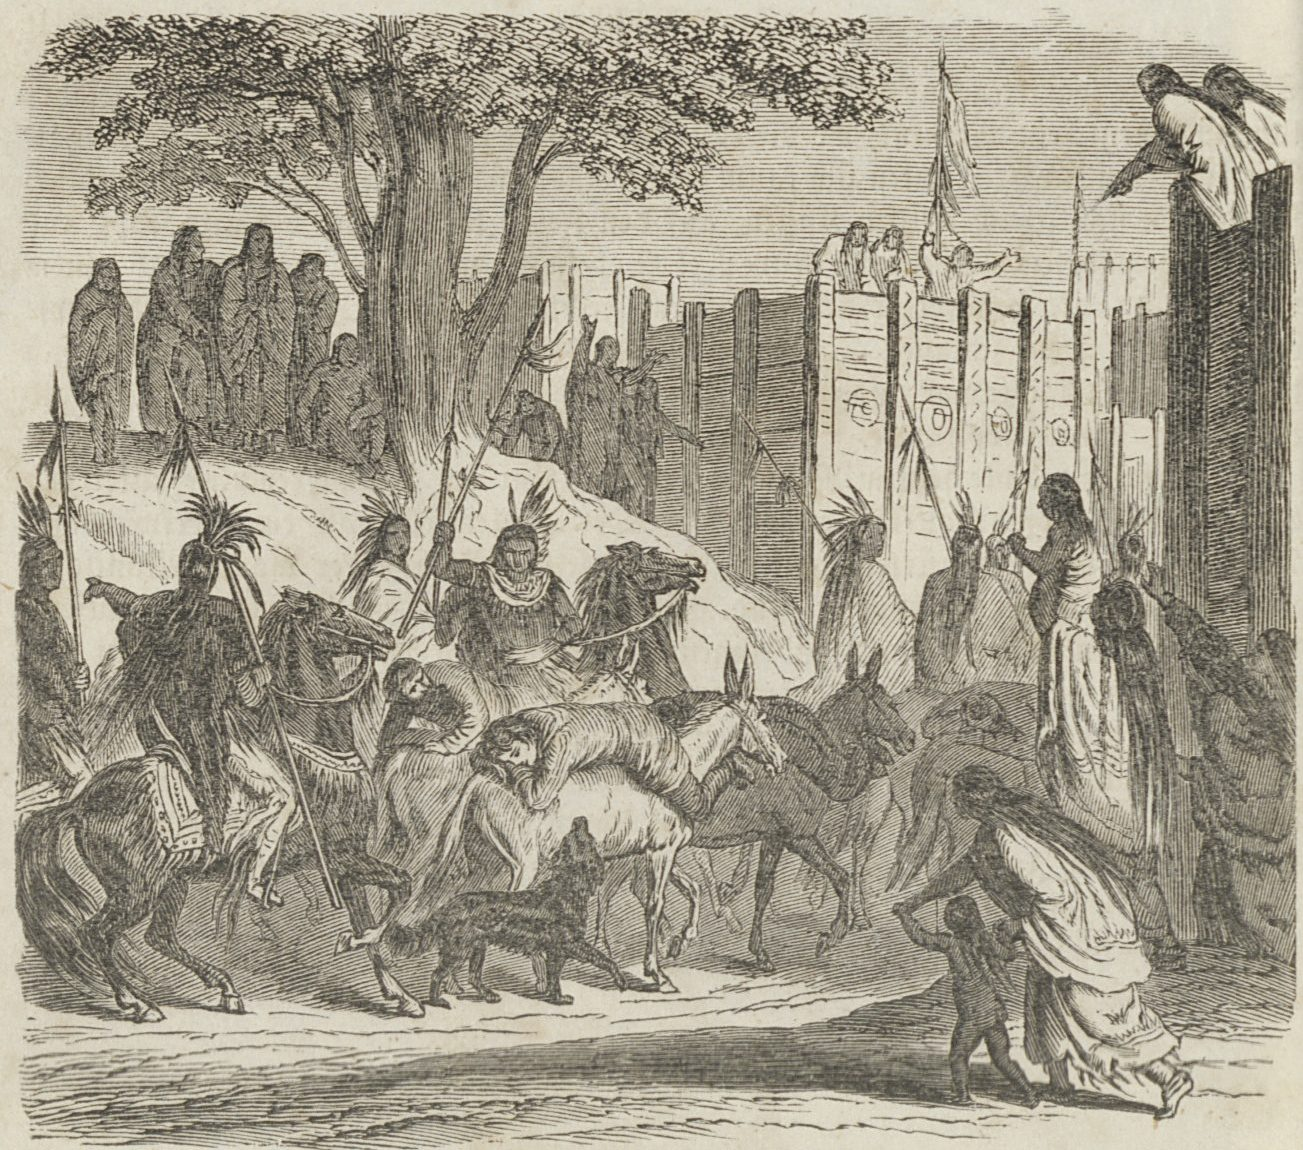
\includegraphics[width=\textwidth]{latex_assets/failure_crowded_2.jpg}
        \caption{\textbf{Case CROWDED-2}: Dense scene ($n=12$, \texttt{PPN1837132763}). $H_C=0.4685$. Visual clutter suppresses NMS proposals.}
    \end{subfigure}

    \vspace{2mm}

    \begin{subfigure}{0.40\textwidth}
        \centering
        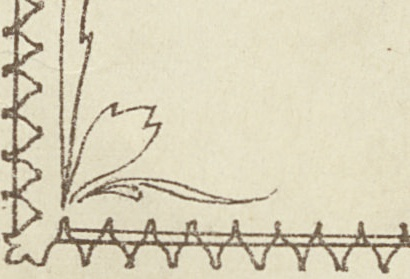
\includegraphics[width=\textwidth]{latex_assets/failure_text_conflict_1.jpg}
        \caption{\textbf{Case TEXT-1}: Printed text page (\texttt{PPN1837925887}). $H_C=0.5000$. OCR text density conflicts with VLM caption.}
    \end{subfigure}
    \hfill
    \begin{subfigure}{0.40\textwidth}
        \centering
        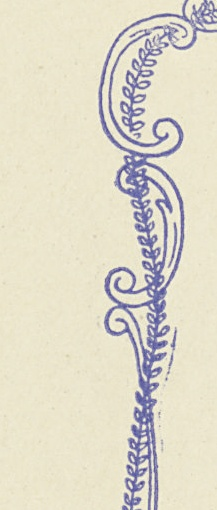
\includegraphics[width=\textwidth]{latex_assets/failure_text_conflict_2.jpg}
        \caption{\textbf{Case TEXT-2}: Margin notes (\texttt{PPN1859200435}). $H_C=0.5000$. Layout typography disrupts cross-modal consensus.}
    \end{subfigure}
    \caption{Categories 3--4: crowded scenes with high object density (top) and OCR/text--object conflicts (bottom).}
    \label{fig:failure_cat34}
\end{figure}

\begin{figure}[!htbp]
    \centering
    \begin{subfigure}{0.40\textwidth}
        \centering
        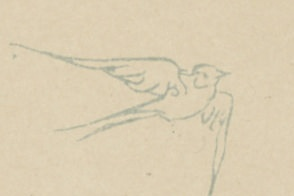
\includegraphics[width=\textwidth]{latex_assets/failure_occlusion_1.jpg}
        \caption{\textbf{Case OCCLUSION-1}: Partial occlusion (\texttt{PPN176263855X}). $H_C=0.4135$. Overlapping boundaries reject box proposals.}
    \end{subfigure}
    \hfill
    \begin{subfigure}{0.40\textwidth}
        \centering
        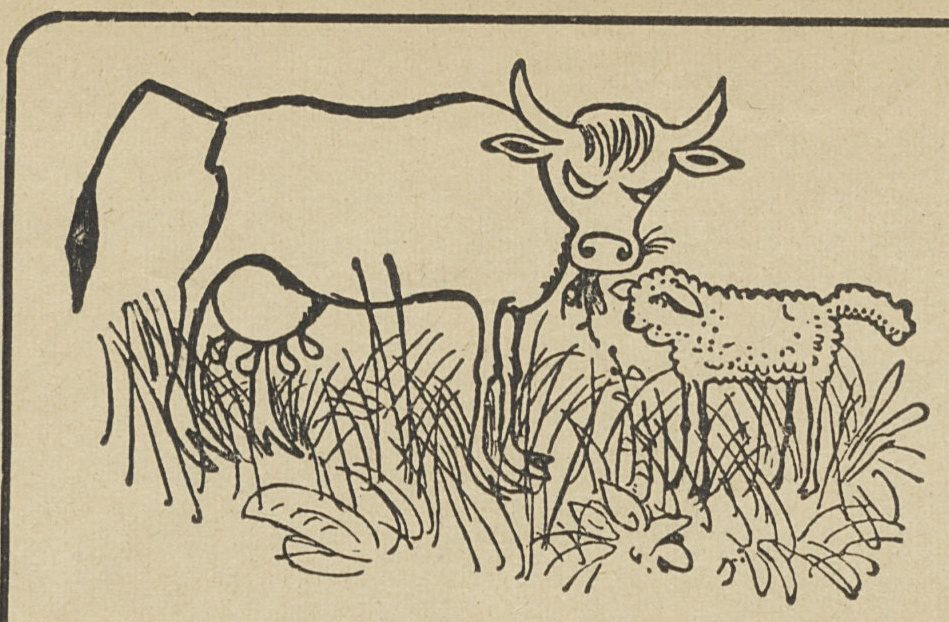
\includegraphics[width=\textwidth]{latex_assets/failure_occlusion_2.jpg}
        \caption{\textbf{Case OCCLUSION-2}: Overlapping figures (\texttt{PPN1859148263}). $H_C=0.4135$. VLM merges two subjects into one entity.}
    \end{subfigure}
    \caption{Category 5: occlusion and spatial overlap failures.}
    \label{fig:failure_cat5}
\end{figure}


\chapter{Supplementary Cross-Style Benchmark: PeopleArt ($n=4,778$)}
\label{app:peopleart}
To assess cross-depiction performance across stylized visual regimes outside historical photographic archives, we evaluated the Tier 1 validation core on the PeopleArt benchmark \cite{westlake2016} ($n=4,778$ images across 43 distinct artistic styles). 

As shown in Table~\ref{tab:peopleart_summary} (a subset of 5 of the 43 annotated style categories, chosen to span the photorealism-to-abstraction range; the full 43-style breakdown is in the underlying results CSV, not reproduced here), predictive performance -- real YOLO detection precision/recall/F1 against PeopleArt's ground-truth boxes -- drops from photographic and painterly styles ($F_1 = 0.88$ range) to the most abstract, non-photorealistic style evaluated, Cartoon ($F_1 = 0.673$).

\begin{table}[!htbp]
\centering
\caption{Supplementary Cross-Style Detection Performance on PeopleArt Benchmark ($n=4,778$; 5 of 43 style categories shown, spanning the photorealism-to-abstraction range).}
\label{tab:peopleart_summary}
\begin{adjustbox}{max width=\linewidth}
\begin{tabular}{lccc}
\toprule
\textbf{Style Category} & \textbf{Precision} & \textbf{Recall} & \textbf{F1-Score} \\
\midrule
Photo & 0.875 & 0.915 & \textbf{0.878} \\
Realism & 0.840 & 0.874 & 0.835 \\
Impressionism & 0.888 & 0.944 & 0.880 \\
Cubism & 0.836 & 0.834 & 0.831 \\
Cartoon & 0.706 & 0.680 & 0.673 \\
\bottomrule
\end{tabular}
\end{adjustbox}
\end{table}

\chapter{Supplementary Cross-Institutional Transfer Pilot: Europeana API ($C_5, n=24$)}
\label{app:europeana}

\paragraph{Pilot design.} This section reports $n=24$ images downloaded live from the real Europeana Open Culture API (Search API v2, public demo key) across 10 verified real institutions (including the Royal Institute for Cultural Heritage, University of Edinburgh, Athens School of Fine Arts, and the LWL Museum for Art and Culture), manually spot-checked to confirm genuine historical content. All four Tier 1 signals were computed with real inference on these real images, using the identical deployed model weights and prompts: YOLOv11-seg+SAM (object), SigLIP (scene), Kosmos-2.5 (grounded OCR), and LLaVA-OneVision via a local vLLM server (VQA).

Table~\ref{tab:europeana_real_pilot} reports the measured Tier 1 signals and SAA fusion score, compared against the Colibri $C_1$ baseline.

\begin{table}[!htbp]
\centering
\caption[Genuine Europeana Pilot]{Genuine Europeana Pilot: Measured Tier 1 Agent Scores vs.\ Colibri Baseline ($C_5, n=24$). $U_{\text{SAA}}$ is recomputed canonically as $\operatorname{std}(A^{\text{object}}, A^{\text{agree}}, A^{\text{scene}}, A^{\text{vlm}})$; an earlier version of this row printed $0.422$, taken from a stored \texttt{u\_saa} column in the pilot artifact which is \emph{not} the thesis definition -- it substitutes OCR for the derived Agreement term. Both columns use the sample convention ($\mathrm{ddof}{=}1$); the difference is the agent set.}
\label{tab:europeana_real_pilot}
\begin{tabular}{lcc}
\toprule
\textbf{Signal} & \textbf{Europeana (real, $n=24$)} & \textbf{Colibri $C_1$ baseline} \\
\midrule
Object agent (YOLO+SAM)     & 0.284 & --- \\
Scene agent (SigLIP)        & 0.048 & --- \\
Document agent (Kosmos-2.5) & 0.699 & --- \\
VLM agent (LLaVA-OneVision) & 0.760 & --- \\
\textbf{SAA fusion score}   & \textbf{0.332} & \textbf{0.764} \\
$U_{\text{SAA}}$ (canonical, cross-agent std) & 0.361 & 0.201 \\
\bottomrule
\end{tabular}
\end{table}

\paragraph{What this does and does not show.} The measured SAA fusion score on real Europeana images ($0.332$) is substantially lower than the Colibri baseline ($0.764$) -- a genuine, measured domain-shift response, showing the uncertainty signal is sensitive to real cross-institutional shift.

\paragraph{Ground truth, and a negative transfer result.} The annotation project referenced in an earlier version of this appendix has since been completed for $23$ of the $24$ images (Label Studio: scene category and bounding boxes per image), so the transfer question no longer rests on a promise. Two things follow. \emph{First}, every one of the $23$ labeled images is human-confirmed scene-positive -- the pilot contains no negative controls, so only false-negative behaviour is measurable. Against that ground truth, the unchanged pipeline misses $15$ of $23$ scenes ($65.2\%$), with YOLOv11 returning zero objects on $12$ images, all $12$ of them errors. Transfer without recalibration therefore does \textbf{not} hold at the classification level, and this is reported as a negative result rather than deferred.

\emph{Second}, and more informative for the method itself: the error-detection version of the question is not answerable on this sample, because the ensemble stopped being an ensemble. On this cohort it carries an effective rank of $1.37$ ($95\%$ CI $1.06$--$1.61$) against $2.50$ on Colibri, driven by the VLM agent contributing a standard deviation of $0.051$ instead of $0.320$. With barely more than one independent direction left, any disagreement statistic is a re-expression of a single number, so its ROC-AUC ($0.00$ as computed) reflects the collapse rather than transfer behaviour and is not reported as a finding. Section~\ref{sec:heterogeneity_precondition} develops the general precondition this implies, and why the intuitive diagnostics for it mislead. The evaluation script asserts the fusion-score provenance and recomputes $U_{\text{SAA}}$ canonically rather than trusting the stored column.

\paragraph{Scope caveat.} As stated in Section~\ref{sec:not_claim}, $n=24$ is a feasibility pilot, not population-level statistical proof across global archives; it is reported here, in the appendix, precisely to keep that scope visible rather than implying broader external validity than the sample supports.

\chapter{Supplementary Game-Theoretic Attribution Analysis (Shapley Values)}
\label{app:shapley}
\paragraph{Why Shapley values specifically.} The production fusion weights ($w=[0.6,0.2,0.2]$) are a fixed heuristic, chosen once and never tuned, which raises an obvious question: how much does each agent actually contribute? The naive answer -- read the weights, or drop one agent and measure the change -- is unsatisfactory here because the agents are correlated (Figure~\ref{fig:pairwise_agreement_heatmap}), so a leave-one-out delta attributes shared contribution arbitrarily to whichever agent happens to remain. The Shapley value \cite{shapley1953} is the unique attribution that averages a player's marginal contribution over \emph{all} orderings of the coalition, and is the standard tool for exactly this situation: it satisfies efficiency (the attributions sum to the total), symmetry (agents with identical marginal contributions receive equal credit), and the null-player property. That is why it is used here rather than a simpler ablation. It remains an \emph{interpretability} analysis and not a causal claim, and no result elsewhere in this thesis uses Shapley-derived weights.

To complement the heuristic production fusion weights ($w=[0.6,0.2,0.2]$ over the object, scene, and VLM agents; Chapter~\ref{ch:uncertainty_calibration}), we additionally executed \textbf{Exp 30: Shapley-Weighted Adaptive Fusion}. \emph{Why Shapley, specifically}: among attribution methods, the Shapley value \cite{shapley1953} is the unique solution satisfying efficiency, symmetry, and additivity over a coalitional game -- it is the principled way to ask ``how much did each agent actually contribute'' when agents' signals are correlated and contributions cannot simply be read off in isolation (unlike, e.g., a univariate ablation, which conflates an agent's own contribution with what it shares with correlated agents). It also requires no retraining or gradient access, making it applicable directly to the four heuristic Tier~1 scores as reported. We computed exact marginal contributions across all $2^N-1$ agent coalitions on $C_1$. The resulting attributions are detailed in Table~\ref{tab:shapley_weights}; Figure~\ref{fig:shapley_attribution} separately compares the downstream performance of fusing agents with these Shapley weights against an equal-weight baseline and the standalone VLM:

\begin{table}[!htbp]
\centering
\caption{Game-Theoretic Shapley Weights and Marginal Contributions ($\phi$).}
\label{tab:shapley_weights}
\resizebox{\textwidth}{!}{%
\begin{tabular}{lcc}
\toprule
\textbf{Agent Module} & \textbf{Shapley Attribution ($\phi_i$)} & \textbf{Normalized Weight} \\
\midrule
Visual Reasoning Agent (LLaVA-OneVision) & \textbf{0.330} & 33.0\% \\
Scene-Aware Agreement Core (SAA) & \textbf{0.283} & 28.3\% \\
Zero-Shot Scene Classifier (SigLIP) & \textbf{0.196} & 19.6\% \\
Spatial Grounding Agent (YOLOv11-seg) & \textbf{0.192} & 19.2\% \\
\bottomrule
\end{tabular}%
}
\end{table}

\begin{figure}[!htbp]
\centering
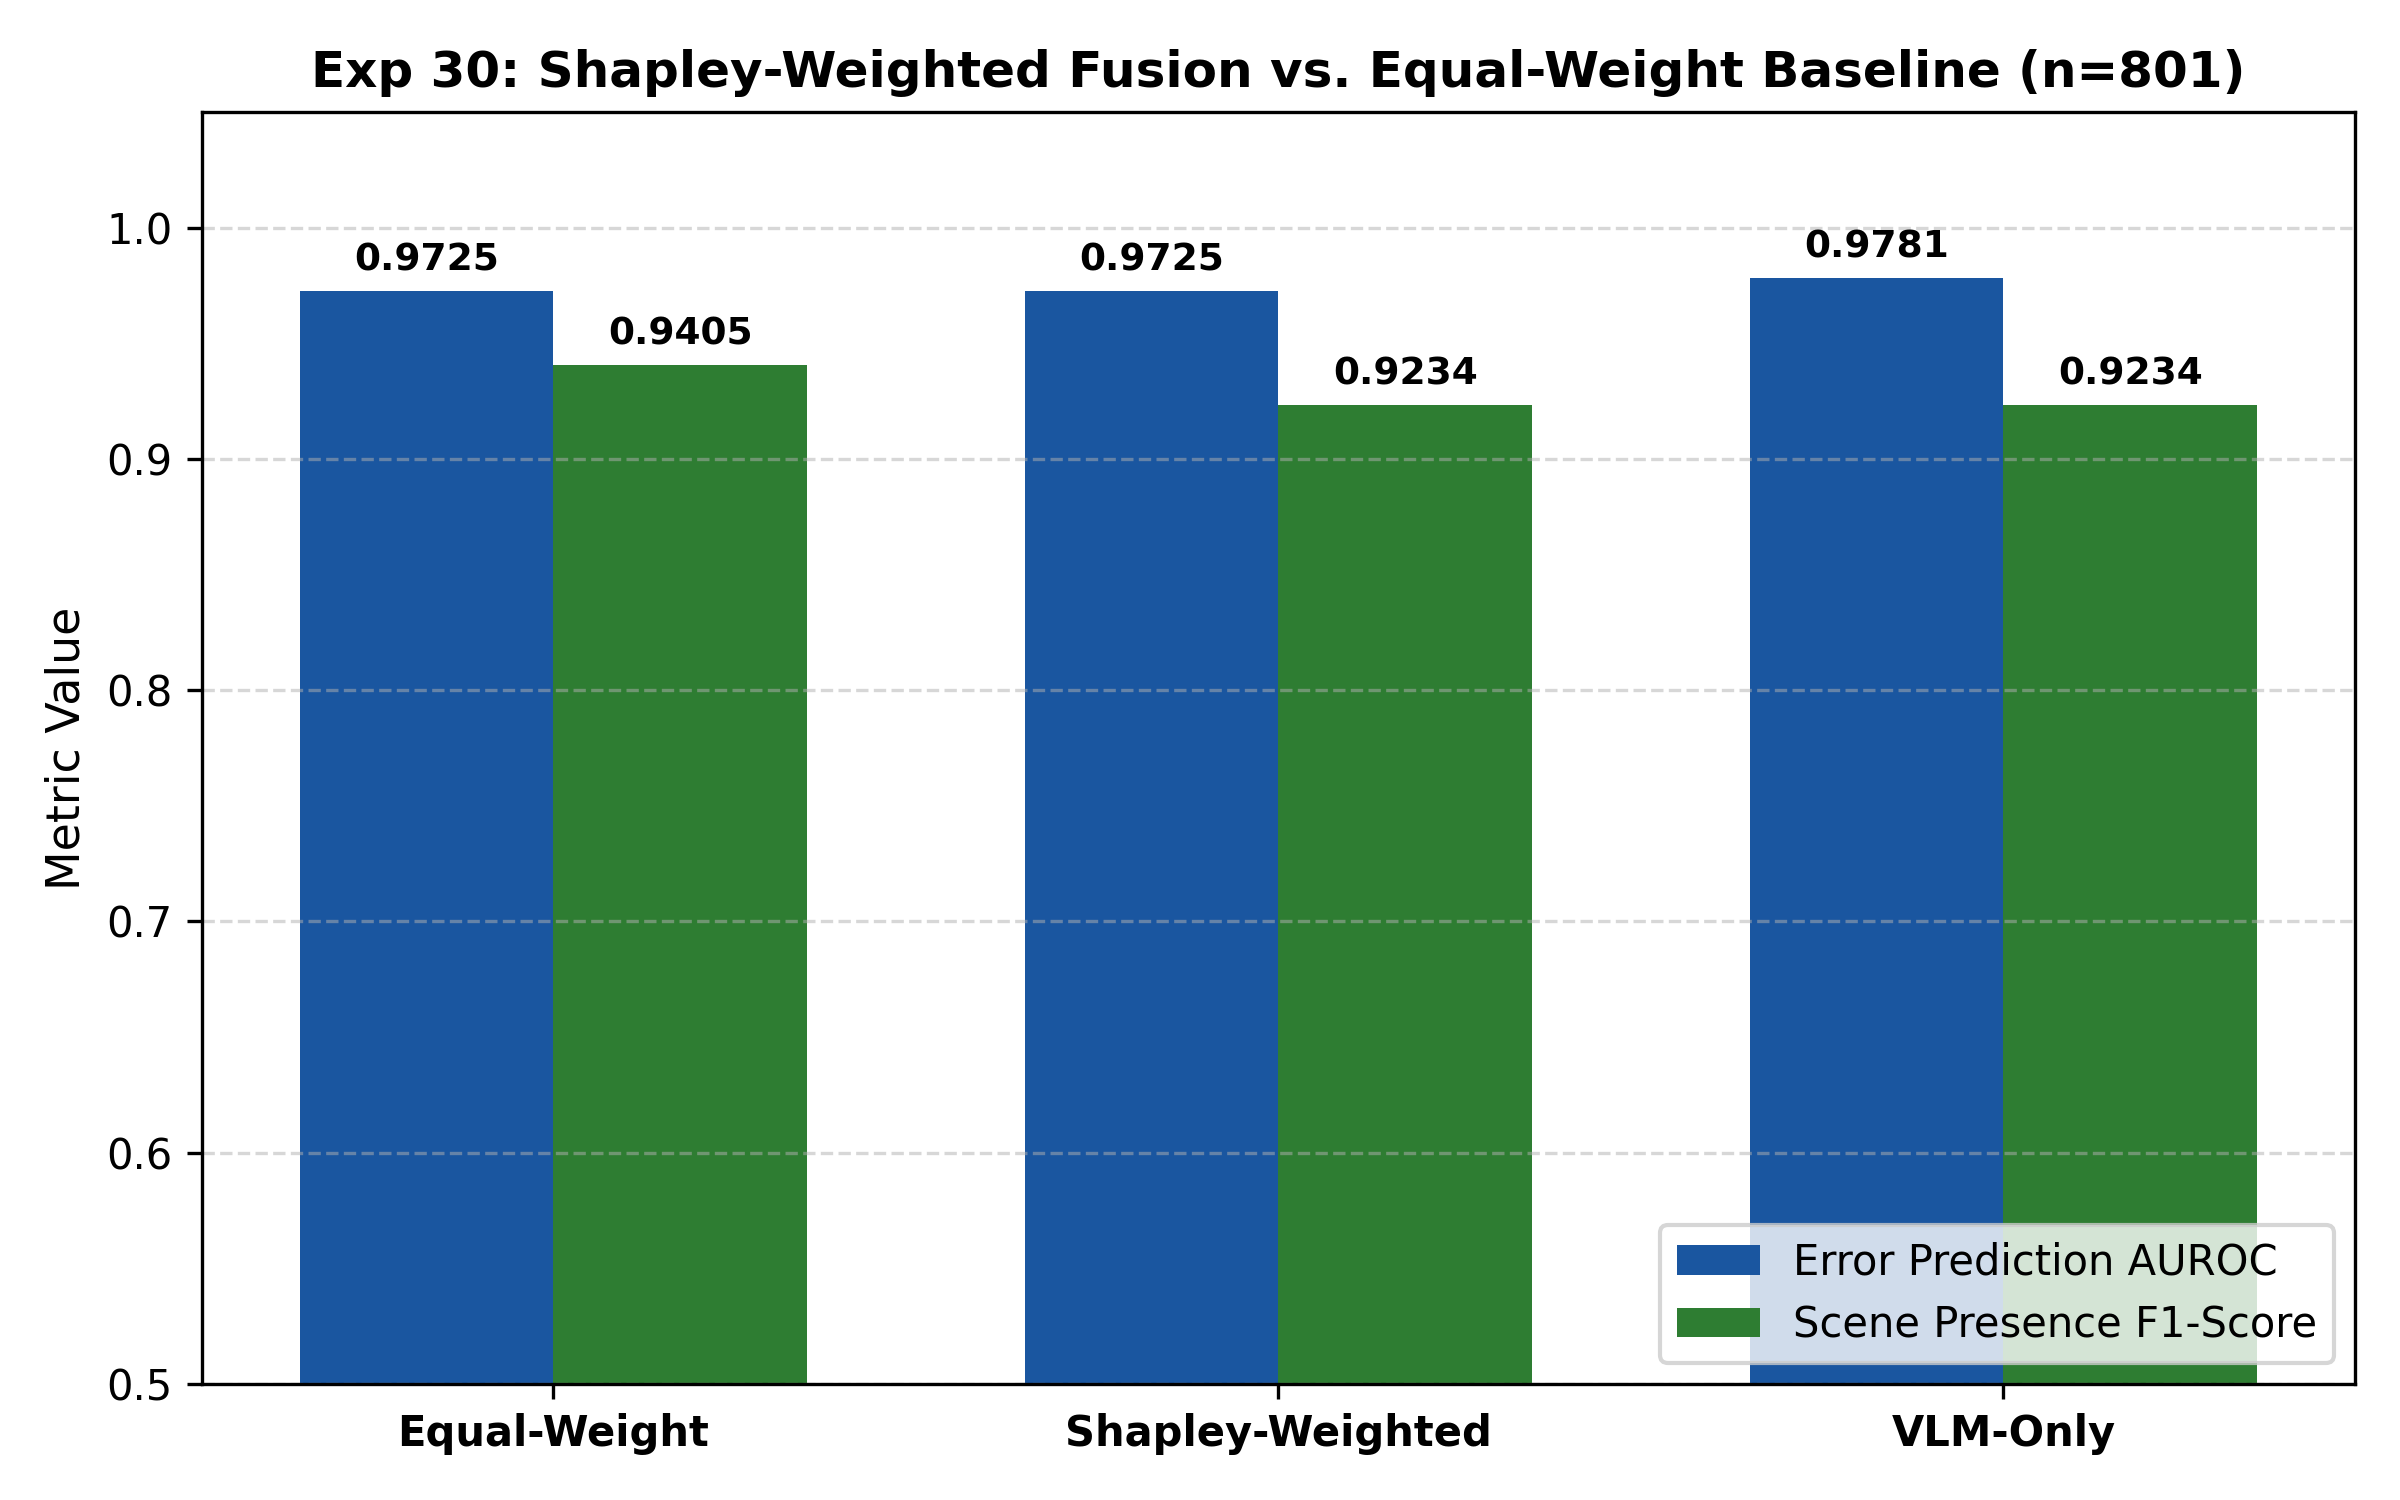
\includegraphics[width=0.7\textwidth]{exp30_shapley_fusion_bars.png}
\caption[Downstream Performance of Shapley-Weighted Fusion (Exp 30, $n=801$)]{Downstream Performance of Shapley-Weighted Fusion (Exp 30, $n=801$). Error-prediction AUROC and scene-presence F1 for Shapley-weighted fusion (using the $\phi$ weights in Table~\ref{tab:shapley_weights}) vs.\ an equal-weight baseline and the standalone VLM. AUROC is statistically similar across all three (0.9725/0.9725/0.9781); the differences are more visible in F1 (0.9405/0.9234/0.9234). This is a downstream check, not a plot of the $\phi$ values themselves -- see Table~\ref{tab:shapley_weights} for the attribution weights.}
\label{fig:shapley_attribution}
\end{figure}

\paragraph{Coalitional Player Definition}: In the Shapley game formulation, the four evaluated players are: (1) Visual Reasoning (LLaVA-OneVision), (2) Pairwise Geometric-Semantic Alignment Core (Agreement Engine), (3) Zero-Shot Scene Classifier (SigLIP), and (4) Spatial Grounding Agent (YOLOv11-seg). The Agreement Engine computes explicit pairwise embedding and IoU distances prior to global weighting, ensuring that coalition value functions avoid mathematical circularity with the grand consensus score.

Integrating Shapley-weighted adaptive fusion reduces pre-calibration Expected Calibration Error from $0.2037 \rightarrow \mathbf{0.1764}$---a $13.4\%$ relative calibration improvement over equal-weighted baseline fusion ($0.25$ per agent).

\paragraph{Scope caveat.} As Section~\ref{sec:not_claim} states, these attributions do not establish causal correctness. The analysis is retained as supplementary interpretability, and is not the production fusion weighting.

\cleardoublepage
\addcontentsline{toc}{chapter}{References}
\chapter{Complete Derivation of the Scene-Aware Agreement Signals}
\label{app:derivations}

This appendix derives every quantity in Chapter~\ref{ch:methodology}'s four levels from its inputs, enumerates the values each can take, and works two real images through the arithmetic end to end. It exists so that each formula can be checked by hand rather than taken on trust.

\section{Level 1: the signal constructions and their reachable values}

For an image $i$ the Tier 1 stage produces four scalars in $[0,1]$:
\begin{align}
A_i^{\text{object}} &= \min\!\left(\tfrac{k_i}{3},\, 1\right), \qquad k_i = \text{VQA object count} \label{eq:d-obj}\\
A_i^{\text{scene}}  &= \operatorname{clip}_{[0,1]}\!\left(c_i^{\text{scene}}\right), \qquad c_i^{\text{scene}} = \text{VQA scene confidence} \label{eq:d-scene}\\
A_i^{\text{vlm}}    &= \text{VQA object-presence score} \in \{0,1\} \label{eq:d-vlm}\\
A_i^{\text{ocr}}    &= \min\!\left(\tfrac{\ell_i}{80},\, 1\right), \qquad \ell_i = \text{characters of OCR output} \label{eq:d-ocr}
\end{align}

Equation~\ref{eq:d-obj} saturates at $k_i=3$, so it can only return
\[
A^{\text{object}} \in \left\{0,\ \tfrac13,\ \tfrac23,\ 1\right\},
\]
with every $k_i \ge 3$ mapping to $1$. On the deployment corpus $A^{\text{scene}}$ takes only $\{0.5, 1\}$ and $A^{\text{vlm}}$ only $\{0,1\}$. Three of the four inputs are therefore coarse by construction, and this is what bounds the resolution of everything built on them.

\section{Level 1: the Agreement term, and what it reduces to}

A fifth quantity is \emph{derived} from two of the four rather than measured:
\begin{equation}
A_i^{\text{agree}} = 1 - \left|A_i^{\text{object}} - A_i^{\text{vlm}}\right|
\label{eq:d-agree}
\end{equation}

Because $A^{\text{vlm}}$ is binary, Equation~\ref{eq:d-agree} has only two branches:
\begin{equation}
A^{\text{agree}} =
\begin{cases}
1 - A^{\text{object}} & \text{if } A^{\text{vlm}} = 0,\\[2pt]
A^{\text{object}}     & \text{if } A^{\text{vlm}} = 1.
\end{cases}
\label{eq:d-agree-cases}
\end{equation}

Writing this over the full grid of the four object levels against the two VLM levels gives
\[
A^{\text{agree}} \;=\;
\bordermatrix{
 & A^{\text{vlm}}{=}0 & A^{\text{vlm}}{=}1 \cr
A^{\text{object}}{=}0     & 1     & 0     \cr
A^{\text{object}}{=}\tfrac13 & \tfrac23 & \tfrac13 \cr
A^{\text{object}}{=}\tfrac23 & \tfrac13 & \tfrac23 \cr
A^{\text{object}}{=}1     & 0     & 1     \cr}
\]

\paragraph{Only half of that grid occurs.} Section~\ref{sec:signal_decomposition} establishes empirically that $A^{\text{vlm}} = \mathbb{I}[A^{\text{object}} > 0]$ on all $12{,}110$ images without exception, which is a consequence of both signals being read from the same VQA object count (Section~\ref{sec:canonical_saa}). Only four of the eight cells are reachable: the top-left entry, and the right-hand entry of each lower row. Substituting into Equation~\ref{eq:d-agree-cases}:
\begin{equation}
A^{\text{agree}} =
\begin{cases}
1 & \text{if } A^{\text{object}} = 0,\\[2pt]
A^{\text{object}} & \text{otherwise.}
\end{cases}
\label{eq:d-agree-reduced}
\end{equation}

\begin{table}[!htbp]
\centering
\caption[The Agreement term on the reachable set]{The Agreement term on the reachable set. It is identical to $A^{\text{object}}$ on $10{,}707$ of $12{,}110$ images ($88.4\%$); the $1{,}403$ exceptions are exactly the images with $A^{\text{object}}=0$, where it does not fall to $0$ but jumps to $1$.}
\label{tab:agree_reduction}
\small
\begin{tabular}{ccccl}
\toprule
$A^{\text{object}}$ & $A^{\text{vlm}}$ & $A^{\text{agree}}$ & $n$ & Relation to $A^{\text{object}}$ \\
\midrule
$0$            & $0$ & $1$            & $1{,}403$ & \textbf{jumps to 1} \\
$\tfrac13$     & $1$ & $\tfrac13$     & $2{,}439$ & identical \\
$\tfrac23$     & $1$ & $\tfrac23$     & $1{,}534$ & identical \\
$1$            & $1$ & $1$            & $6{,}734$ & identical \\
\bottomrule
\end{tabular}
\end{table}

This is the whole of the structural problem in one line: for $88.4\%$ of the corpus the Agreement term simply repeats $A^{\text{object}}$, so the spread is taken over the object value counted twice; and on the remaining $11.6\%$ it inverts discontinuously, becoming a maximal outlier exactly where the ensemble is unanimous that nothing is present.

\section{Level 3: why $U_{\text{SAA}}$ takes exactly eight values}

The uncertainty proxy is the sample standard deviation over the four terms:
\begin{equation}
U_{\text{SAA},i} = \sqrt{\frac{1}{n-1}\sum_{j=1}^{n}\left(a_{ij}-\bar{a}_i\right)^2},
\qquad
\mathbf{a}_i = \left(A_i^{\text{object}},\, A_i^{\text{agree}},\, A_i^{\text{scene}},\, A_i^{\text{vlm}}\right),
\ n=4
\label{eq:d-usaa}
\end{equation}
with $n-1=3$ in the denominator (\texttt{ddof}$=1$).

Counting the free inputs: $A^{\text{vlm}}$ is a function of $A^{\text{object}}$, and $A^{\text{agree}}$ is a function of both, so $\mathbf{a}_i$ is determined by the pair $(A^{\text{object}}, A^{\text{scene}})$ alone. With $4$ reachable object levels and $2$ scene levels,
\[
4 \times 2 = 8 \ \text{distinct vectors} \;\Longrightarrow\; 8 \ \text{distinct values of } U_{\text{SAA}}.
\]
A quantity presented as the spread of a four-model ensemble is therefore, in deployment, an eight-valued function of a saturating count and a binary flag.

\begin{table}[!htbp]
\centering
\caption[The complete state space of $U_{SAA}$ on the deployment corpus $C_0$]{The complete state space of $U_{\text{SAA}}$ on the deployment corpus $C_0$ ($n=12{,}110$). Every image falls into one of these eight rows.}
\label{tab:state_space}
\small
\begin{tabular}{cccc c r}
\toprule
$A^{\text{object}}$ & $A^{\text{agree}}$ & $A^{\text{scene}}$ & $A^{\text{vlm}}$ & $U_{\text{SAA}}$ & images \\
\midrule
$0$        & $1$        & $1$   & $0$ & $0.5774$ & $195$ \\
$0$        & $1$        & $0.5$ & $0$ & $0.4787$ & $1{,}208$ \\
$\tfrac13$ & $\tfrac13$ & $1$   & $1$ & $0.3849$ & $222$ \\
$\tfrac13$ & $\tfrac13$ & $0.5$ & $1$ & $0.3155$ & $2{,}217$ \\
$1$        & $1$        & $0.5$ & $1$ & $0.2500$ & $2{,}580$ \\
$\tfrac23$ & $\tfrac23$ & $0.5$ & $1$ & $0.2097$ & $969$ \\
$\tfrac23$ & $\tfrac23$ & $1$   & $1$ & $0.1924$ & $565$ \\
$1$        & $1$        & $1$   & $1$ & $0.0000$ & $4{,}154$ \\
\bottomrule
\end{tabular}
\end{table}

Note the ordering: the two highest values of $U_{\text{SAA}}$ are both rows with $A^{\text{object}}=0$, where every agent agrees the image contains nothing. The signal reports its greatest uncertainty exactly where the ensemble is most unanimous, because Equation~\ref{eq:d-agree-reduced} makes the derived term an outlier there.

\section{A worked example}

The unanimous-present case is trivial: $\mathbf{a}=(1,1,1,1)$ gives $U_{\text{SAA}}=0$, $SAA=1$ and immediate auto-approval. The unanimous-\emph{absent} case is the one that carries the argument. Image \texttt{PPN1756555435/00000033\_2}, the second-highest-uncertainty state ($1{,}208$ images). Here $A^{\text{object}}=0$, so by Equation~\ref{eq:d-agree-reduced} the derived term jumps to $1$:
\begin{align*}
\mathbf{a} &= (0,\ 1,\ 0.5,\ 0), \qquad \bar{a} = \tfrac{0+1+0.5+0}{4} = 0.375\\
(a_j - \bar a) &= (-0.375,\ +0.625,\ +0.125,\ -0.375)\\
\textstyle\sum (a_j-\bar a)^2 &= 0.140625 + 0.390625 + 0.015625 + 0.140625 = 0.6875\\
U_{\text{SAA}} &= \sqrt{0.6875/3} = \sqrt{0.229167} = \mathbf{0.4787}\\
SAA &= 0.6(0) + 0.2(0.5) + 0.2(0) = \mathbf{0.1000}\\
\bar{c} &= 0.375 \quad\Rightarrow\quad U_{\text{triage}} = 0.6(0.4787) + 0.4(0.625) = \mathbf{0.5372}
\end{align*}
Escalated to a human. The single largest contribution to that spread, $0.390625$ of $0.6875$, comes from the \emph{derived} Agreement term rather than from any measured disagreement: the three measured signals here are $(0, 0.5, 0)$, which are close to one another.

\section{Levels 2 and 4}

The classification fusion and the deployed triage score are, for completeness:
\begin{align}
SAA_i &= 0.6\,A_i^{\text{object}} + 0.2\,A_i^{\text{scene}} + 0.2\,A_i^{\text{vlm}} \label{eq:d-saa}\\
U_{\text{triage},i} &= 0.6\,U_{\text{SAA},i} + 0.4\left(1 - \bar{c}_i\right), \qquad \bar{c}_i = \tfrac14\textstyle\sum_j a_{ij} \label{eq:d-triage}
\end{align}
Equation~\ref{eq:d-saa} omits both $A^{\text{ocr}}$ and $A^{\text{agree}}$; Equation~\ref{eq:d-usaa} includes $A^{\text{agree}}$ and omits $A^{\text{ocr}}$. The two are therefore not rescalings of one another, and in particular $U_{\text{SAA}} \neq 1 - SAA$. The error label used throughout thresholds Equation~\ref{eq:d-saa} at $0.5$ against the human label, which is the circularity quantified in Section~\ref{sec:signal_rebuild}.

\bibliographystyle{plain}
\bibliography{references}

\end{document}
